%%%%%%%%%%%%%%%%%%%%%%%%%%%%%%%%%%%%%%%%%%%%%%%%%%%%%%%%%%%%%%%%%%%%%%%%%%%%%%%%%
%
% Purpose:  Top level document for \DerivedStateDesc.  DO NOT EDIT!!!
%
% 
%
%%%%%%%%%%%%%%%%%%%%%%%%%%%%%%%%%%%%%%%%%%%%%%%%%%%%%%%%%%%%%%%%%%%%%%%%%%%%%%%%


\documentclass[twoside,11pt,titlepage]{report}

%
% Bring in the AMS math package
%
\usepackage{amsmath,amssymb,amsfonts,textcomp}

%
% Bring in the common page setup
%
\usepackage{dynenv}

%
% Bring in the common math nomenclature
%
\usepackage{dynmath}

%
% Bring in the model-specific commands
%
\usepackage{derived_state}

%
% Bring in the graphics environment
%
\usepackage{graphicx}

%
% Bring in the hyper ref environment
%
\usepackage[colorlinks,plainpages=false,verbose]{hyperref}
%  keywords for pdfkeywords are separated by commas
\hypersetup{
   pdftitle={\DerivedStateDesc},
   pdfauthor={\ModelAuthor},
   pdfkeywords={\ModelKeywords},
   pdfsubject={\DerivedStateDesc}}

\begin{document}

%%%%%%%%%%%%%%%%%%%%%%%%%%%%%%%%%%%
% Front matter
%%%%%%%%%%%%%%%%%%%%%%%%%%%%%%%%%%%
\pagenumbering{roman}

\docid{models/dynamics/derived\_state}
\docrev{1.1}
\date{\RELEASEMONTH\ \RELEASEYEAR}
\modelname{\DerivedStateDesc}
\doctype{}
\author{\ModelAuthor}
\managers{
  Robert O. Shelton \\ Project Manager \\
  Michael T. Red \\ Simulation and Graphics Branch Chief \\
  R. Matt Ondler \\ Software, Robotics, and Simulation Division Chief}
\pdfbookmark{Title Page}{titlepage}
\makeDynenvTitlepage

\pdfbookmark{Abstract}{abstract}
%%%%%%%%%%%%%%%%%%%%%%%%%%%%%%%%%%%%%%%%%%%%%%%%%%%%%%%%%%%%%%%%%%%%%%%%%%%%%%%%%
%
% Purpose:  Abstract for the DerivedState model
%
% 
%
%%%%%%%%%%%%%%%%%%%%%%%%%%%%%%%%%%%%%%%%%%%%%%%%%%%%%%%%%%%%%%%%%%%%%%%%%%%%%%%%


\section*{Abstract}

When describing the state of a vehicle, we are describing the translational and rotational position and
velocity with respect to some reference frame.  For simplicity, the integration
of a vehicular state is performed in an inertial reference frame, but the input
and output of that state may be expressed in any of a boundless set of
representations, such as LVLH or Orbital Elements.  The Derived State model provides the capability to express a
vehicular state in one or more of the most frequently used representations, and
the extension capability to define other representations not released with
\JEODid.



\pdfbookmark{Contents}{contents}
\tableofcontents
\vfill

\pagebreak

%%%%%%%%%%%%%%%%%%%%%%%%%%%%%%%%%%%
% Main Document Body
%%%%%%%%%%%%%%%%%%%%%%%%%%%%%%%%%%%
\pagenumbering{arabic}




\part{Overview}

%----------------------------------
\chapter{Introduction}\hyperdef{part}{intro}{}\label{ch:intro}
%----------------------------------

\section{Purpose and Objectives of the \DerivedStateDesc}
%%%%%%%%%%%%%%%%%%%%%%%%%%%%%%%%%%%%%%%%%%%%%%%%%%%%%%%%%%%%%%%%%%%%%%%%%%%%%%%%%
%
% Purpose:  Introduction for the DerivedState model.
%
%
%
%%%%%%%%%%%%%%%%%%%%%%%%%%%%%%%%%%%%%%%%%%%%%%%%%%%%%%%%%%%%%%%%%%%%%%%%%%%%%%%%


%\section{Purpose and Objectives of \DerivedStateDesc}
% Incorporate the intro paragraph that used to begin this Chapter here.
% This is location of the true introduction where you explain what this model
% does.

The Derived State model provides the capability to express a
vehicular state in one or more of the most frequently used reference frame concepts (such as LVLH), with respect to another object included in the simulation.  While effort has been made to identify and include those reference frame representations most frequently utilized in orbital dynamics simulations, we recognize that we have not provided complete coverage of what is a boundless number of possible representations, and so have provided the flexibility that allows for the further definition of additional reference frame representations for inclusion into the model as needed.

The following reference frame representations are included in the \DerivedStateDesc:

\begin{enumerate}
\item{\EulerDesc}
\item{\LVLHDesc}
\item{\NEDDesc}
\item{\OrbElemDesc}
\item{\PlanetaryDesc}
\item{\RelativeDesc}
\item{\SolarBetaDesc}
\end{enumerate}


\section{Context within JEOD}
The following document is parent to this document:
\begin{itemize}
\item{\href{file:\JEODHOME/docs/JEOD.pdf}
           {\em JSC Engineering Orbital Dynamics}}
			  \cite{dynenv:JEOD}
\end{itemize}

The \DerivedStateDesc\ forms a component of the \ModelClass\ suite of
models within \JEODid. It is located at
models/\ModelClass/derived\_state.  

\section{Documentation History}
%%%%%%%%%%%%%%%%%%%%%%%%%%%%%%%%%%%%%%%%%%%%%%%%%%%%%%%%%%%%%%%%%%%%%%%%%%%%%%%%%
%
% Purpose:  Change history for document for the DerivedState model
%
% 
%
%%%%%%%%%%%%%%%%%%%%%%%%%%%%%%%%%%%%%%%%%%%%%%%%%%%%%%%%%%%%%%%%%%%%%%%%%%%%%%%%


%\section{Documentation History}
%%% Status of this and only this document.  Any date should be
%relevant to when 
%%% this document was last updated and mention the reason (release,
%bug fix, etc.)
%%% Mention previous history aka JEOD 1.4-5 heritage in this section.

\begin{tabular}{||l|l|l|l|} \hline
 {\bf Author} & {\bf Date} &  {\bf Revision} & {\bf Description} \\ \hline \hline
 Gary Turner & November, 2009 & 1.0  & JEOD2.0.0 release \\ \hline
 Robert Shelton & April, 2016 & 1.1  & Added Documentation for LVLH Relative Derived State \\ \hline
\end{tabular}



\section{Documentation Organization}
This document is formatted in accordance with the 
NASA Software Engineering Requirements Standard~\cite{NASA:SWE}.  The document comprises several parts.  The first part is an overview of the model; each subsequent part describes a sub-model of the \DerivedStateDesc, with each sub-model representing an independent reference frame or state representation.  Each part is organized into a similar structure, comprising the following chapters in order:

\begin{description}
%% longer chapter descriptions, more information.

\item[Introduction] - 
This introduction describes the objective and purpose of the object of the respective part; the introduction in Part I - Overview also contains the document history.

\item[Product Requirements] -
Describes requirements for the object of the respective part.

\item[Product Specification] -
Describes the underlying theory, architecture, and design of the
object of the respective part in detail.  It will be organized into the following sections:
\begin{itemize}
 \item Conceptual Design.
 \item Mathematical Formulations.
 \item Detailed Design.
 \item Version Inventory (Part I - Overview only).
\end{itemize}
 

\item[User's Guide] -
Describes how to use the object of the respective part in a Trick simulation.  The User's Guide for each sub-model
is divided into three sections to represent the JEOD defined user types:
\begin{itemize}
 \item Analysts or users of simulations (Analysis).
 \item Integrators or developers of simulations (Integration).
 \item Model Extenders (Extension).
\end{itemize}
 
\item[Verification and Validation] -
Contains verification and validation procedures and
results for the object of the resepctive part.

\end{description}


%----------------------------------
\chapter{Product Requirements}\hyperdef{part}{spec}{}\label{ch:reqt}
%----------------------------------

\requirement{Top-level requirement}
\label{reqt:top_level}
\begin{description}
\item[Requirement:]\ \newline
  This model shall meet the JEOD project requirements specified in
  the \JEODid\
  \hyperref{file:\JEODHOME/docs/JEOD.pdf}{part1}{reqt}{ top-level
  document}.
\item[Rationale:]\ \newline
  This model shall, at a minimum,  meet all external and
  internal requirements 
  applied to the \JEODid\ release.
\item[Verification:]\ \newline
  Inspection 
\end{description}


%%%%%%%%%%%%%%%%%%%%%%%%%%%%%%%%%%%%%%%%%%%%%%%%%%%%%%%%%%%%%%%%%%%%%%%%%%%%%%%%%
%
% Purpose:  requirements for the DerivedState model
%
% 
%
%%%%%%%%%%%%%%%%%%%%%%%%%%%%%%%%%%%%%%%%%%%%%%%%%%%%%%%%%%%%%%%%%%%%%%%%%%%%%%%%

% add text here to describe general model requirements
% text is of the form:
%\requirement{REQUIREMENT DESCRIPTION}
%\label{reqt:REQT_DESC_ABBREVIATED}
%\begin{description}
%  \item[Requirement:]\ \newline
%     <Insert description of requirement> 
%  \item[Rationale:]\ \newline
%     <Insert description of rationale> 
%  \item[Verification:]\ \newline
%     <Insert description of verification (e.g. "Inspection")> 
%\end{description}

\requirement{Minimal Functionality}
\label{reqt:DerivedState_min_func}
\begin{description}
  \item[Requirement:]\ \newline
     The \JEODid\ release of the \DerivedStateDesc\ shall include, at a minimum, the same functionality as was available in version JEODv1.5.2.
  \item[Rationale:]\ \newline
     The new framework should not detract from the functionality of the package.
  \item[Verification:]\ \newline
     Inspection.
\end{description}

\section{Requirements Traceability}\label{sec:traceability}

\begin{longtable}[c]{||p{3.5in}|p{3.5in}|}
\caption{Requirements Traceability} \\[6pt]
\hline
{\bf Requirement} & {\bf Inspection and Testing} \\ 
\hline \hline
\endhead
\ref{reqt:top_level} - Top-level Requirements &
  Insp.~\ref{inspect:top_level} \\ \hline
\ref{reqt:DerivedState_min_func} - Minimum Functionality &
  Insp.~\ref{inspect:DerivedState_min_func} \\ \hline

\end{longtable}




%----------------------------------
\chapter{Product Specification}\hyperdef{part}{spec}{}\label{ch:spec}
%----------------------------------

\section{Conceptual Design}
%%%%%%%%%%%%%%%%%%%%%%%%%%%%%%%%%%%%%%%%%%%%%%%%%%%%%%%%%%%%%%%%%%%%%%%%%%%%%%%%%
%
% Purpose:  Conceptual part of Product Spec for the DerivedState model
%
% 
%
%%%%%%%%%%%%%%%%%%%%%%%%%%%%%%%%%%%%%%%%%%%%%%%%%%%%%%%%%%%%%%%%%%%%%%%%%%%%%%%%


%\section{Conceptual Design}
The \DerivedStateDesc\ shall provide the interface by which the state of any given object can be expressed in any given reference frame, or a new reference frame created with respect to any other reference frame if the desired representation is not already available.  Two of the sub-classes (\LVLHDesc\ and \NEDDesc) are specialized to the point of providing only a reference frame; two (\PlanetaryDesc\ and \SolarBetaDesc) are closely tied to planetary bodies and rely on the pre-definition of those reference frames; \OrbElemDesc\ provides the state of a vehicle in classical orbital elements, and tacitly assumes that there is a planetary body involved for the vehicle to be orbiting; the other two (\EulerDesc\ and \RelativeDesc) express the state of one reference frame relative to any other.

The generic Derived State provides a name for the state, based on entries it receives from the sub-classes for the names of the \textit{subject frame} (the reference frame associated with the vehicle whose state is to be enumerated) and the \textit{reference frame} (the frame in which that state is to be evaluated).  Each of the specific examples of derived states will inherit from the generic derived state, specifying those frames (although the reference frame need not be specified for all instances), thereby providing the data to the generic DerivedState for generating the state name.  Excepting the \LVLHDesc\ and the \NEDDesc\, each example of a DerivedState will then output a set of values that identify those parts of the subject's state for which it is responsible.  The \LVLHDesc\ and \NEDDesc\ define their respective reference frames, for access by a state-generating Derived State, such as the \RelativeDesc.

While the sub-classes of Derived State (i.e., the reference frames and state representations) are largely independent of one another, there are places where there is some interdependency, and the methods and definitions from one sub-class are similar to, or dependent upon, methods and definitions from another class.  In those situations, links to the documentation appropriate to the situation are included as necessary.
%\section{Mathematical Formulations}
%%%%%%%%%%%%%%%%%%%%%%%%%%%%%%%%%%%%%%%%%%%%%%%%%%%%%%%%%%%%%%%%%%%%%%%%%%%%%%%%%
%
% Purpose:  Mathematical Formulation part of Product Spec for the DerivedState model
%
% 
%
%%%%%%%%%%%%%%%%%%%%%%%%%%%%%%%%%%%%%%%%%%%%%%%%%%%%%%%%%%%%%%%%%%%%%%%%%%%%%%%%

\section{Mathematical Formulations}

The top-level DerivedState class contains no mathematical manipulations.  All of the mathematics in this model is handled within the appropriate sub-class.  See the individual Mathematical Formulations sections in the respective parts of this document for details.

%\section{Detailed Design}

%%%%%%%%%%%%%%%%%%%%%%%%%%%%%%%%%%%%%%%%%%%%%%%%%%%%%%%%%%%%%%%%%%%%%%%%%%%%%%%%%
%
% Purpose:  Detailed part of Product Spec for the DerivedState model
%
% 
%
%%%%%%%%%%%%%%%%%%%%%%%%%%%%%%%%%%%%%%%%%%%%%%%%%%%%%%%%%%%%%%%%%%%%%%%%%%%%%%%%

\section{Detailed Design}
\label{ref:DerivedState}

\subsection{Functional Design}
See the \href{file:refman.pdf}{Reference Manual}\cite{derivedstatebib:ReferenceManual} for a summary of member data and member methods for all classes.  This section describes the functional operation of the methods identified in the base-class, DerivedState.

The Derived State provides common functionality to its sub-classes.

\begin{itemize}
\funcitem{find\_planet}
Uses the Dynamics Manager method \textit{find\_planet} to find a planet with name \textit{planet\_name}
\funcitem{initialize}
The \textit{initialize} method receives a reference to the subject body and to the dynamics manager.  Its primary responsibility is to set the identifying name of the state, \textit{state\_identifier}.  This comprises the following elements:
\begin{enumerate}
\item{The type name}\ \newline
The type name would be something like \textit{LvlhDerivedState}, or \textit{RelativeDerivedState}.
\item{The name of the subject body}\ \newline
This is set by the user, often in the input file, or a Modified data file.  Both are included in the verification simulations:  for example, the Solar Beta verification simulation uses the input file (textit{verif/SIM\_SolarBeta/SET\_test/RUN\_comp\_ISS/input})
\begin{verbatim}
veh.dyn_body.set_name( "solar_beta_test_vehicle" );
\end{verbatim}
whereas the LVLH verification simulation uses a Modified Data file entry \newline (\textit{verif/SIM\_LVLH/Modified\_data/veh.d})
\begin{verbatim}
veh.dyn_body.set_name( "vehicle1" );
\end{verbatim}

\item{The reference name \textit{(optional)}}\ \newline
The reference name is used in identifying a reference frame by name, and in naming the state identifier.  By coincidence, for those sub-classes of DerivedState included in \JEODid\, when the reference name is being used to identify a reference frame, it is always used to identify a planet.  However, this is a coincidence, not a rule; it is not set in stone and any extensions to \JEODid\ need not adhere to this statement.

Not all subclasses of DerivedState require the \textit{reference\_name} in all situations, some require it only when the user requires something other than the default reference frame, and some never require it.  For those subclasses and situations that do not require a reference name, the inclusion of one will only be used in the state identifier.  Those that do not have a defined reference name will have only a 2-member identifier, whereas those with a reference name will have a 3-member identifier.  This value is also set by the user, again usually in the input file or a Modified data file.
For example, from \textit{verif/SIM\_SolarBeta/SET\_test/RUN\_comp\_ISS/input}:
\begin{verbatim}
veh.solar_beta.reference_name = "Earth";
\end{verbatim}
\end{enumerate}

Continuing with the example from
\textit{verif/SIM\_SolarBeta/SET\_test/RUN\_comp\_ISS/input},
the simulation has a SolarBetaDerivedState, for which this initialize method is called.  The resulting \textit{state\_identifier} value that is output is
\begin{verbatim}
SolarBetaDerivedState.solar_beta_test_vehicle.Earth
\end{verbatim}
\funcitem{update}
This method is included for consistency; it has no other purpose.
\funcitem{validate\_name}
Used by \textit{find\_planet} to ensure that names have been specified.
\end{itemize}

%\section{Version Inventory}
%%%%%%%%%%%%%%%%%%%%%%%%%%%%%%%%%%%%%%%%%%%%%%%%%%%%%%%%%%%%%%%%%%%%%%%%%%%%%%%%%
%
% Purpose:  Inventory of files for the DerivedState model
%
% 
%
%%%%%%%%%%%%%%%%%%%%%%%%%%%%%%%%%%%%%%%%%%%%%%%%%%%%%%%%%%%%%%%%%%%%%%%%%%%%%%%%

\section{Inventory}
All \DerivedStateDesc\ files are located in the directory \newline
{\tt \$\{JEOD\_HOME\}/models/dynamics/derived\_state}.
Relative to this directory,
\begin{itemize}
\vspace{-0.2\baselineskip}
\item Header and source files are located
in the model {\tt include} and {\tt src} subdirectories.
Table~\ref{tab:source_files} lists the
configuration-managed files in these directories.
\vspace{-0.1\baselineskip}
\item Documentation files are located in the model {\tt docs} subdirectory.
See table~\ref{tab:documentation_files}
for a listing of the
configuration-managed files in this directory.
\vspace{-0.1\baselineskip}
\item Verification files are located in the model {\tt verif} subdirectory.
See table~\ref{tab:verification_files}
for a listing of the
configuration-managed files in this directory.
\end{itemize}

\input{inventory}


\chapter{User's Guide}\hyperdef{part}{user}{}\label{ch:user}
%----------------------------------
The top level of the \DerivedStateDesc\ should not be used directly in a simulation.  Specific instances of the \DerivedStateDesc\ should be used instead, although the implementation varies from instance to instance.  See the User's Guides in the respective Part of this document for details of specific implementation.

%----------------------------------
\chapter{Verification and Validation}\hyperdef{part}{ivv}{}\label{ch:ivv}
%----------------------------------

\section{Verification}
%%%%%%%%%%%%%%%%%%%%%%%%%%%%%%%%%%%%%%%%%%%%%%%%%%%%%%%%%%%%%%%%%%%%%%%%%%%%%%%%%
%
% Purpose:  Verification part of V&V for the DerivedState model
%
% 
%
%%%%%%%%%%%%%%%%%%%%%%%%%%%%%%%%%%%%%%%%%%%%%%%%%%%%%%%%%%%%%%%%%%%%%%%%%%%%%%%%

% \section{Verification}

%%% code imported from old template structure
\inspection{Top-level Requirement}\label{inspect:top_level}
 This document structure, the code, and associated files have been inspected, and together satisfy requirement~\ref{reqt:top_level}.

\inspection{Minimum Functionality}\label{inspect:DerivedState_min_func}
 This model provides:
\begin{enumerate}

 \item The following reference frames:
\begin{enumerate}
 \item Local-Vertical-Local-Horizontal (LVLH)
\item North-East-Down(NED)
\end{enumerate}

\item The translational states in the following formats, using reference frames defined elsewhere in \JEODid:
\begin{enumerate}
 \item Classical Orbital Elements
 \item Planetary altitude-latitude-longitude
\end{enumerate}

\item The rotational states utilizing a sequence of 3 rotation angles about coordinate axes, 

\item The Solar Beta angle associated with any given state, 

\item The ability to express the state of one reference frame in terms of another.

\end{enumerate}  

Together, these capabilities satisfy requirement~\ref{reqt:DerivedState_min_func}.

%\section{Validation}
%%%%%%%%%%%%%%%%%%%%%%%%%%%%%%%%%%%%%%%%%%%%%%%%%%%%%%%%%%%%%%%%%%%%%%%%%%%%%%%%%
%
% Purpose:  Validation part of V&V for the DerivedState model
%
% 
%
%%%%%%%%%%%%%%%%%%%%%%%%%%%%%%%%%%%%%%%%%%%%%%%%%%%%%%%%%%%%%%%%%%%%%%%%%%%%%%%%

\section{Validation}

%%% code imported from old template structure
%\test{<Title>}\label{test:<label>}
%\begin{description}
%\item[Purpose:] \ \newline
%<description>
%\item[Requirements:] \ \newline
%By passing this test, the universal time module 
%partially satisfies requirement~\ref{reqt:<label1>} and 
%completely satisfies requirement~\ref{reqt:<label2>}.
%\item[Procedure:]\ \newline
%<procedure>
%\item[Results:]\ \newline
%<results>
%\end{description}

Validation, where applicable, is performed for the specific implementations of the model.  See the Validation sections in each respective Part of this document for validation data appropriate to each sub-class.

\section{Metrics}
\subsection{Code Metrics}

Table~\ref{tab:coarse_metrics} presents coarse metrics on the
source files that comprise the model.

\input{coarse_metrics}

Table~\ref{tab:metrix_metrics} presents the extended cyclomatic
complexity
(ECC) of the methods defined in the model.
\input{metrix_metrics}



\part{\EulerDescT}



%----------------------------------
\chapter{Introduction}\label{ch:Eulerintro}
%----------------------------------

\section{Purpose and Objectives of the \EulerDescT}
%%%%%%%%%%%%%%%%%%%%%%%%%%%%%%%%%%%%%%%%%%%%%%%%%%%%%%%%%%%%%%%%%%%%%%%%%%%%%%%%%
%
% Purpose:  Introduction for the Euler model.
%
% 
%
%%%%%%%%%%%%%%%%%%%%%%%%%%%%%%%%%%%%%%%%%%%%%%%%%%%%%%%%%%%%%%%%%%%%%%%%%%%%%%%%


%\section{Purpose and Objectives of \EulerDesc}
% Incorporate the intro paragraph that used to begin this Chapter here. 
% This is location of the true introduction where you explain what this model 
% does.
The Euler Derived State represents the relative attitude of a particular reference frame with respect to some other frame as a series of Euler angle rotations.  The output will be a 3-vector of angles; the user may specify in which order those angles are to be expressed.

















%----------------------------------
\chapter{Product Requirements}\label{ch:Eulerreqt}
%----------------------------------


%%%%%%%%%%%%%%%%%%%%%%%%%%%%%%%%%%%%%%%%%%%%%%%%%%%%%%%%%%%%%%%%%%%%%%%%%%%%%%%%%
%
% Purpose:  requirements for the Euler model
%
% 
%
%%%%%%%%%%%%%%%%%%%%%%%%%%%%%%%%%%%%%%%%%%%%%%%%%%%%%%%%%%%%%%%%%%%%%%%%%%%%%%%%

% add text here to describe general model requirements
% text is of the form:
\requirement{Calculate relative attitude between two reference frames}
\label{reqt:Euler}
\begin{description}
  \item[Requirement:]\ \newline
     Given a reference frame associated with a body, the \EulerDesc\ will calculate an Euler-type angle sequence from body frame to the reference frame parent to it, and from the parent frame to the body frame using the 3 basic axes, represented as roll(x-axis rotation), pitch (y-axis rotation), and yaw (z-axis rotation).
  \item[Rationale:]\ \newline
     To provide a means of expressing relative attitude between reference frames.
  \item[Verification:]\ \newline
     Test
\end{description}

\section{Requirements Traceability}

\begin{longtable}[c]{||p{3.5in}|p{3.5in}|}
\caption{Requirements Traceability} \\[6pt]
\hline
{\bf Requirement} & {\bf Inspection and Testing} \\ 
\hline \hline
\endhead
\ref{reqt:Euler} - Calculate relative attitude between two reference frames &
  Test~\ref{test:Euler} \\ \hline
\end{longtable}




%----------------------------------
\chapter{Product Specification}\label{ch:Eulerspec}
%----------------------------------

\section{Conceptual Design}
%%%%%%%%%%%%%%%%%%%%%%%%%%%%%%%%%%%%%%%%%%%%%%%%%%%%%%%%%%%%%%%%%%%%%%%%%%%%%%%%%
%
% Purpose:  Conceptual part of Product Spec for the Euler model
%
% 
%
%%%%%%%%%%%%%%%%%%%%%%%%%%%%%%%%%%%%%%%%%%%%%%%%%%%%%%%%%%%%%%%%%%%%%%%%%%%%%%%%


%\section{Conceptual Design}
A reference frame attitude can be described as a set of three rotations about independent axes.  In the \EulerDesc\, the Roll, Pitch, and Yaw axes are used, and can be input in any order \textbf{without repeats} (i.e. all three axes must be used).  Numerically, three values are specified in a single vector, corresponding to the angle of rotation about each specified axis in turn.

The angles represent a process for conducting a transformation from one reference frame to another, thereby providing data on the relative attitude of the two frames.  Because the relative attitude can be expressed in either direction, two sets of angles, \textit{ref\_body\_angles} and \textit{body\_ref\_angles} are included in the available output.  \textit{ref\_body\_angles} provides the transformation from the external reference frame to the subject-body reference frame, and \textit{body\_ref\_angles} provides the reverse transformation.

When calculating the Euler angles from two reference frames, both sets of angles are calculated.

%\section{Mathematical Formulations}
%%%%%%%%%%%%%%%%%%%%%%%%%%%%%%%%%%%%%%%%%%%%%%%%%%%%%%%%%%%%%%%%%%%%%%%%%%%%%%%%%
%
% Purpose:  Mathematical Formulation part of Product Spec for the Euler model
%
% 
%
%%%%%%%%%%%%%%%%%%%%%%%%%%%%%%%%%%%%%%%%%%%%%%%%%%%%%%%%%%%%%%%%%%%%%%%%%%%%%%%%

\section{Mathematical Formulations}
The \EulerDesc\ relies on the Trick method \textit{euler\_matrix} for generating the euler angles.  No further mathematical framework is implemented in the \EulerDesc.
%\section{Detailed Design}

%%%%%%%%%%%%%%%%%%%%%%%%%%%%%%%%%%%%%%%%%%%%%%%%%%%%%%%%%%%%%%%%%%%%%%%%%%%%%%%%%
%
% Purpose:  Detailed part of Product Spec for the Euler model
%
% 
%
%%%%%%%%%%%%%%%%%%%%%%%%%%%%%%%%%%%%%%%%%%%%%%%%%%%%%%%%%%%%%%%%%%%%%%%%%%%%%%%%

\section{Detailed Design}

See the \href{file:refman.pdf}{Reference Manual}\cite{derivedstatebib:ReferenceManual} for a summary of member data and member methods for all classes.  

\subsection{Process Architecture}
The process architecture for the \EulerDesc\ is trivial, comprising entirely independent methods.

\subsection{Functional Design}
This section describes the functional operation of the methods in each class.

The \EulerDesc\ contains only one class:
\begin{itemize}
\classitem{EulerDerivedState}
\textref{DerivedState}{ref:DerivedState}

This contains the methods \textit{initialize}, and \textit{update}:
\begin{enumerate}

\funcitem{initialize}
There are two processes for initialization, depending on the relationship in the Reference Frame Tree between the subject-body reference frame, and the exterior reference frame.  If the former is not a child of the latter, then it becomes necessary to specify which frame is to be used as the external reference frame.  In this case, a separate initialization process allows for the specification of that frame.  Otherwise, the initialization process simply calls the generic DerivedState initialization routine to establish the naming convention of the reference object (i.e., the planet about which the vehicle is orbiting) and state identifier.

\funcitem{update}
If the Euler angles are to be computed relative to a frame other than the parent frame, that relative state is first calculated.  Then the Trick method \textit{euler\_matrix} is called for both reference-to-subject and subject-to-reference frame transformations.

\end{enumerate}
\end{itemize}


\chapter{User's Guide}\label{ch:Euleruser}
%----------------------------------
The Analysis section of the User's Guide is intended primarily for
users of pre-existing simulations.  
It contains: 
\begin{itemize}
\item A description of how to modify \EulerDesc\ variables after
the simulation
has compiled, including an in-depth discussion of the input file,
\item An overview of how to interpret (but not edit) the S\_define
file,
\item A sample of some of the typical variables that may be logged.
\end{itemize}

The Integration section of the User's Guide is intended for simulation
developers.
It describes the necessary configuration of the \EulerDesc\
within an
S\_define file, and the creation of standard run directories.  The
latter
component assumes a thorough understanding of the preceding Analysis
section of the user guide.
Where applicable, the user may be directed to selected portions of
Product Specification (Chapter \ref{ch:Eulerspec}).

The Extension section of the User's Guide is intended primarily for
developers
needing to extend the capability of the \EulerDesc.  Such users
should have a
thorough understanding of how the model is used in the preceding
Integration section, and of the model
specification (described in Chapter \ref{ch:Eulerspec}).


\section{Analysis}
%%%%%%%%%%%%%%%%%%%%%%%%%%%%%%%%%%%%%%%%%%%%%%%%%%%%%%%%%%%%%%%%%%%%%%%%%%%%%%%%%
%
% Purpose:  Analysis part of User's Guide for the Euler model
%
% 
%
%%%%%%%%%%%%%%%%%%%%%%%%%%%%%%%%%%%%%%%%%%%%%%%%%%%%%%%%%%%%%%%%%%%%%%%%%%%%%%%%

% \section{Analysis}

\label{sec:euleruseranalysis}
\subsection{Identifying the \EulerDescT}
If the Euler angles have been included in the simulation, there will be an instance of \textit{EulerDerivedState} located in the S\_define file.  This would typically be found in the vehicle object.  There should be an accompanying call to an initialization routine, which takes a reference to the \textit{subject\_body} as one if its inputs, and may also take a reference to a reference-frame, although this is not necessary.  There will also be an accompanying call to an update function.  The essential variable \textit{sequence}, the order in which the angles should be assigned to each axis, is defined elsewhere, often in the input file.

Example:
\begin{verbatim}
sim_object{
dynamics/derived_state:    EulerDerivedState example_of_euler_angles;

(initialization) dynamics/derived_state:
example_of_rel_state_object.example_of_euler_angles.initialize (
    Inout DynBody &      subject_body = vehicle_1.dyn_body,
    Inout DynManager &   dyn_manager  = manager_object.dyn_manager);
    
{environment} dynamics/derived_state:
example_of_rel_state_object.example_of_euler_angles.update ( )

} example_of_rel_state_object;
\end{verbatim}

The input file may contain an entry comparable to:
\begin{verbatim}
example_of_rel_state_object.example_of_euler_angles.sequence = Roll_Pitch_Yaw;
\end{verbatim}
This variable can take one of the following values:
\begin{itemize}
\item{} Roll\_ Pitch\_ Yaw
\item{} Roll\_ Yaw\_ Pitch
\item{} Pitch\_ Yaw\_ Roll
\item{} Pitch\_ Roll\_ Yaw
\item{} Yaw\_ Roll\_ Pitch
\item{} Yaw\_ Pitch\_ Roll
\end{itemize}

\subsection{Editing the \EulerDescT}
The sequence is open to edit by the analyst.

\subsection{Output Data}
The direct output from the \EulerDesc\ comprises only the two vectors of angles,
\textit{ref\_body\_angles} (the Euler angles from the reference frame to the subject frame), and
\textit{body\_ref\_angles} (the Euler angles to the reference frame from the subject frame).
\begin{verbatim}
example_of_rel_state_object.example_of_euler_angles.ref_body_angles[0-2]
example_of_rel_state_object.example_of_euler_angles.body_ref_angles[0-2]
\end{verbatim}





%\section{Integration}
%%%%%%%%%%%%%%%%%%%%%%%%%%%%%%%%%%%%%%%%%%%%%%%%%%%%%%%%%%%%%%%%%%%%%%%%%%%%%%%%%
%
% Purpose:  Integration part of User's Guide for the Euler model
%
% 
%
%%%%%%%%%%%%%%%%%%%%%%%%%%%%%%%%%%%%%%%%%%%%%%%%%%%%%%%%%%%%%%%%%%%%%%%%%%%%%%%%

 \section{Integration}
Simply including the \EulerDesc\ is a trivial undertaking, all of the contents that can be included into the model are identified in the previous section (\ref{sec:euleruseranalysis}).

%\section{Extension}
%%%%%%%%%%%%%%%%%%%%%%%%%%%%%%%%%%%%%%%%%%%%%%%%%%%%%%%%%%%%%%%%%%%%%%%%%%%%%%%%%
%
% Purpose:  Extension part of User's Guide for the Euler model
%
% 
%
%%%%%%%%%%%%%%%%%%%%%%%%%%%%%%%%%%%%%%%%%%%%%%%%%%%%%%%%%%%%%%%%%%%%%%%%%%%%%%%%

 \section{Extension}
The \EulerDesc\ is not written with the intention of being extended.

%----------------------------------
\chapter{Verification and
Validation}\label{ch:Eulerivv}
%----------------------------------

\section{Verification}
%%%%%%%%%%%%%%%%%%%%%%%%%%%%%%%%%%%%%%%%%%%%%%%%%%%%%%%%%%%%%%%%%%%%%%%%%%%%%%%%%
%
% Purpose:  Verification part of V&V for the Euler model
%
% 
%
%%%%%%%%%%%%%%%%%%%%%%%%%%%%%%%%%%%%%%%%%%%%%%%%%%%%%%%%%%%%%%%%%%%%%%%%%%%%%%%%

% \section{Verification}

%%% code imported from old template structure
%\inspection{<Name of Inspection>}\label{inspect:<label>}
% <description> to satisfy  
% requirement \ref{reqt:<label>}.

 For testing the \EulerDesc\, a single vehicle was initialized in one of 3 orbits: an equatorial circular orbit, an inclined orbit, and an eccentric equatorial orbit.  An LVLH frame was also generated, and the Euler angles between the vehicle body frame (the subject frame), and the LVLH frame (the reference frame), were computed.  

\test{Verification of \EulerDesc\ Output Data}\label{test:Euler}

\begin{description}
\item{Purpose:}\newline
To demonstrate that the output from the \EulerDesc\ provides meaningful data.

\item{Requirements:}\newline
Satisfactory conclusion of this test satisfies requirement \ref{reqt:Euler}

\item{Procedure:}\newline
Two cases were considered, one in which the vehicle frame was initially aligned with the LVLH frame, and one in which it was given an initial relative attitude.  In both cases, the vehicle body frame was initialized with no rotation (with respect to the inertial frame).  Since the LVLH frame maintains an orientation dependent upon the position of the origin, the two frames rotate with respect to one another.  The angles generated by this orbital motion are considered.

\item{Predictions:}  
In the LVLH frame, the frame-to-frame relative rotation will appear as a pitch (rotation about the LVLH y-axis).  In the tests in which the two frames are initially aligned, that is equivalent to a pitch in the body frame.  Both transformations should exhibit slowly oscillating pitch values, with constant zero values for yaw and roll.

When the two frames are not initially aligned, in general, the variation of angles resulting from the varying relative attitude will be across all three axes.  Exceptions to this rule include transformations from body to LVLH that end with a pitch, or those from LVLH to body that start with a pitch.  This is due to the order of calculation, consider the transformation from body to LVLH:

The transformation from body to initial LVLH frame is constant, and the LVLH rotates with respect to the initial LVLH frame on its y-axis; a transformation from body to LVLH can be seen as a combination of transformations from body to the initial LVLH frame followed by one from the initial LVLH frame to LVLH, which comprises only a pitch component.  Therefore, if pitch is last in the order, the two pitch adjustments simply add; the roll and yaw are due to the constant difference between body and initial LVLH, and so should remain constant, whereas the pitch should start at some pre-assigned value, and exhibit the same periodic variation thereafter that was seen in the case of the initially aligned frames.  The same argument can be traced in reverse for the reverse transformation.

For other sets in which the pitch is calculated in an inconvenient sequence (second or third, or first from body frame to reference frame, or last in reference frame to body frame), the effect in the yaw and roll angles of the addition of the pitch due to the variational relative frame rotation will manifest as a time dependency on all 3 axes, due to the cross-coupling effects of rotational sequences.

The variation with time in the rate at which the angles change will be constant for the circular orbits, but variable for the elliptic orbits.

For further confirmation of the data, the euler angles of the vehicle with respect to the inertially-oriented planetary axes we investigated, these should show no variation.

\item{Results:}
All output data confirmed expectations, within numerical precision.  Some expected constant values were not quite constant, but exhibited some very small oscillatory or noisy behavior.  

For the aligned frames, the YRP, RYP, PYR, and PRY sequences showed the pitch slowly changing  from $\pm \pi$ to $\mp \pi$ before immediately resetting.  The YPR and RPY sequences had the pitch varying only between $\pm \frac{\pi}{2}$, and doing so with constant ramps up and down.  For these two sequences, the roll and pitch also switched to $\pm \pi$ during the time that the pitch was decreasing, and returned to zero while the pitch was increasing.  These solutions are completely valid, and illustrate that there is more than one way to represent a particular orientation.  These results were valid for both the LVLH-body and body-LVLH orientations. See figures~\ref{fig:euleralignedpyr} and~\ref{fig:euleralignedrpy} for Pitch-Yaw-Roll and Roll-Pitch-Yaw sequences.

\begin{figure}[!ht]
\begin{center}
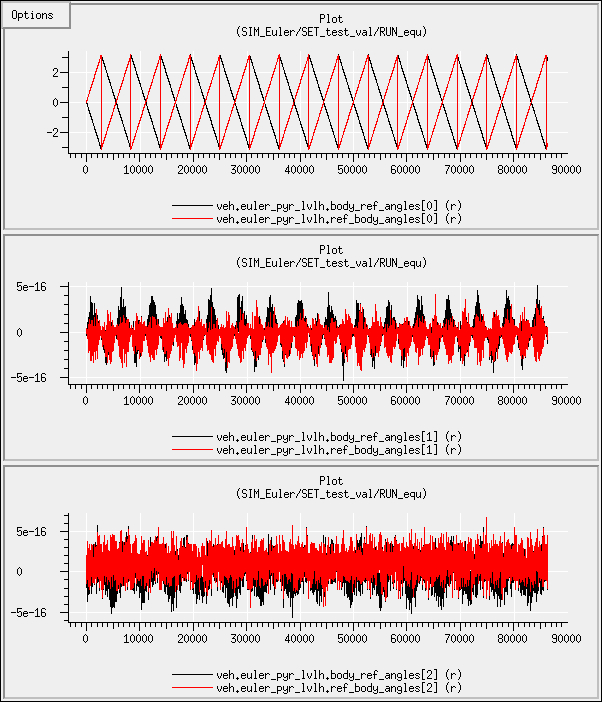
\includegraphics[width=5in]{figures/euler_aligned_pyr.jpg}
\caption{The Euler angles for the case in which the LVLH frame and body frame were initially aligned, and rotating with respect to each other on their respective pitch axes, expressed in a Pitch-Yaw-Roll sequence.}
\label{fig:euleralignedpyr}
\end{center}
\end{figure}

\begin{figure}[!ht]
\begin{center}
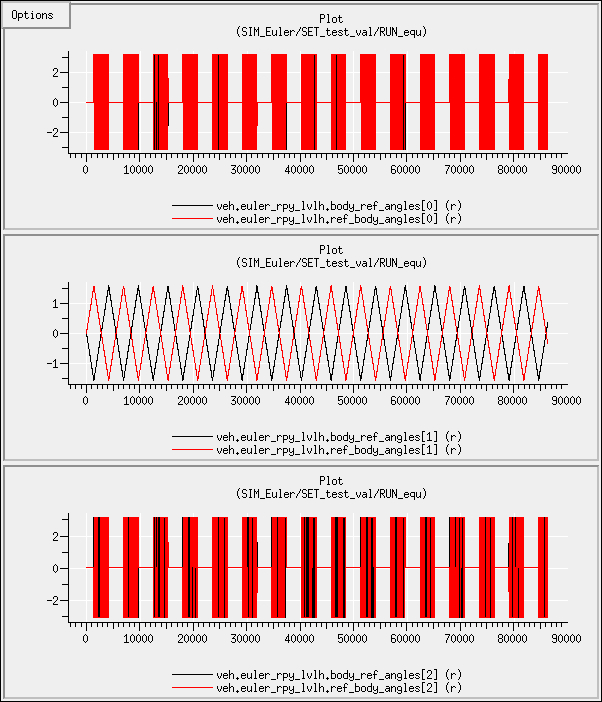
\includegraphics[width=5in]{figures/euler_aligned_rpy.jpg}
\caption{The Euler angles for the case in which the LVLH frame and body frame were initially aligned, and rotating with respect to each other on their respective pitch axes, expressed in a Roll-Pitch-Yaw sequence.  Notice that the Pitch has a total range of only $\pi$ radians; this is compensated for by the combined effect of adding in $\pi$ rotations on the yaw and roll axes.}
\label{fig:euleralignedrpy}
\end{center}
\end{figure}

For the tests in which the frames were not initially aligned, those with Pitch in the correct sequencing showed the similar pattern to the aligned frames, as expected.  Other sequences had periodic behavior.  See Figures~\ref{fig:eulernonalignedpyr},~\ref{fig:eulernonalignedrpy}, and~\ref{fig:eulernonalignedyrp} for Pitch-Yaw-Roll, Roll-Pitch-Yaw, and Yaw-Roll-Pitch sequences.

\begin{figure}[!ht]
\begin{center}
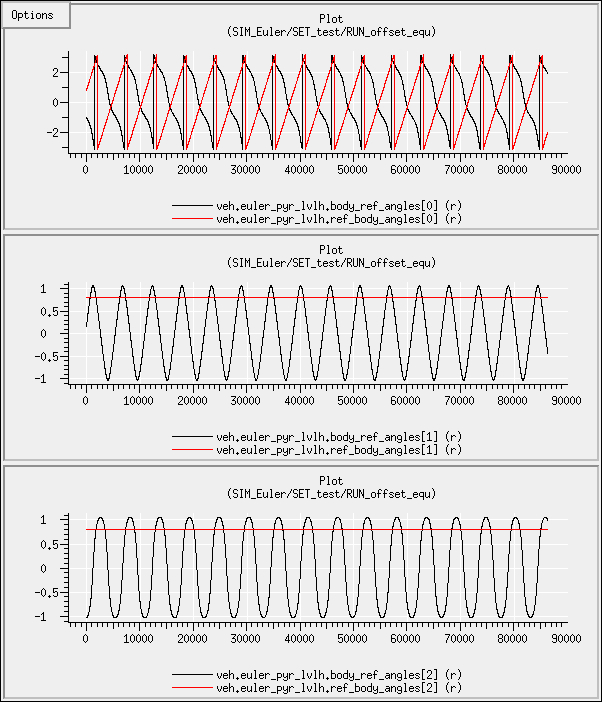
\includegraphics[width=5in]{figures/euler_nonaligned_pyr.jpg}
\caption{The Euler angles for the case in which the LVLH frame and body frame were initially un-aligned, and rotating with respect to each other on the pitch axis of the LVLH reference frame.  Angles are expressed in a Pitch-Yaw-Roll sequence.  Notice that when Pitch is first in the sequence, the angles associated with the transformation from the LVLH frame to the body frame (expressed in the LVLH frame) show a similar pattern to that in Figure~\ref{fig:euleralignedpyr}, but that is not the case when representing the relative attitude from the body frame to the LVLH frame (this is expressed in the body frame).}
\label{fig:eulernonalignedpyr}
\end{center}
\end{figure}

\begin{figure}[!ht]
\begin{center}
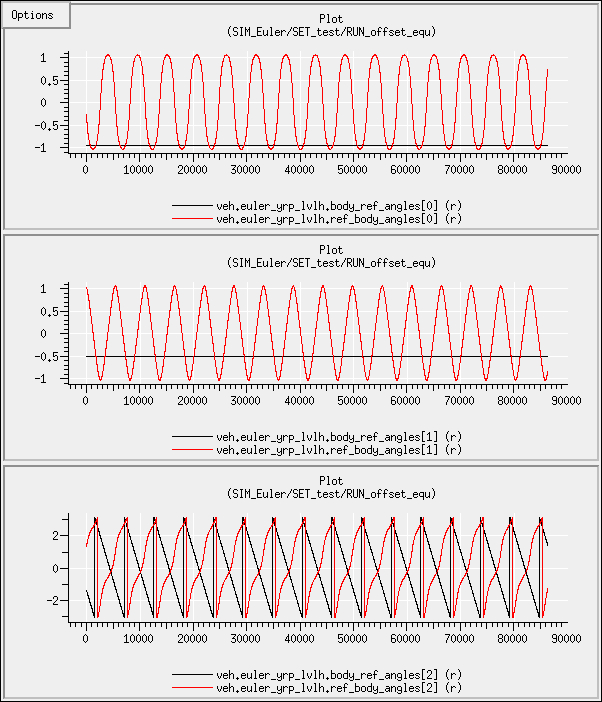
\includegraphics[width=5in]{figures/euler_nonaligned_yrp.jpg}
\caption{The Euler angles for the case in which the LVLH frame and body frame were initially un-aligned, and rotating with respect to each other on the pitch axis of the LVLH reference frame.  Angles are expressed in a Yaw-Roll-Pitch sequence.  Notice that when Pitch is last in the sequence, the angles associated with the transformation from body frame to LVLH (expressed in body frame) show a similar pattern to that in Figure~\ref{fig:euleralignedpyr}, but that is not the case when representing the relative attitude from the LVLH frame to the body frame (this is expressed in the LVLH frame).}
\label{fig:eulernonalignedyrp}
\end{center}
\end{figure}

\begin{figure}[!ht]
\begin{center}
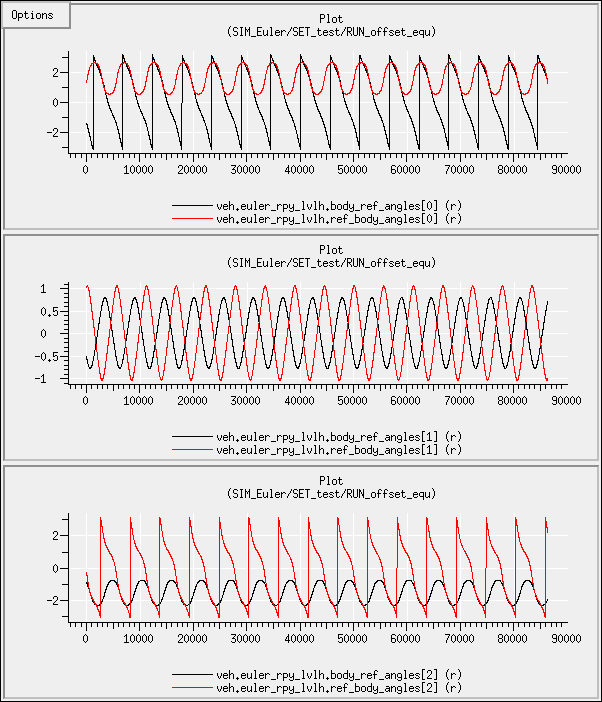
\includegraphics[width=5in]{figures/euler_nonaligned_rpy.jpg}
\caption{The Euler angles for the case in which the LVLH frame and body frame were initially un-aligned, and rotating with respect to each other on the pitch axis of the LVLH reference frame.  Notice that the variation is non-sinusoidal, and that the amplitudes differ between the two representations of the transformation.}
\label{fig:eulernonalignedrpy}
\end{center}
\end{figure}




\end{description}


%\section{Validation}
%%%%%%%%%%%%%%%%%%%%%%%%%%%%%%%%%%%%%%%%%%%%%%%%%%%%%%%%%%%%%%%%%%%%%%%%%%%%%%%%%
%
% Purpose:  Validation part of V&V for the Euler model
%
% 
%
%%%%%%%%%%%%%%%%%%%%%%%%%%%%%%%%%%%%%%%%%%%%%%%%%%%%%%%%%%%%%%%%%%%%%%%%%%%%%%%%

\section{Validation}

There is no independent validation of this sub-model.
%%% code imported from old template structure
%\test{<Title>}\label{test:<label>}
%\begin{description}
%\item[Purpose:] \ \newline
%<description>
%\item[Requirements:] \ \newline
%By passing this test, the universal time module 
%partially satisfies requirement~\ref{reqt:<label1>} and 
%completely satisfies requirement~\ref{reqt:<label2>}.
%\item[Procedure:]\ \newline
%<procedure>
%\item[Results:]\ \newline
%<results>
%\end{description}





\part{\LVLHDesc}



%----------------------------------
\chapter{Introduction}\label{ch:LVLHintro}
%----------------------------------

\section{Purpose and Objectives of the \LVLHDesc}
%%%%%%%%%%%%%%%%%%%%%%%%%%%%%%%%%%%%%%%%%%%%%%%%%%%%%%%%%%%%%%%%%%%%%%%%%%%%%%%%%
%
% Purpose:  Introduction for the LVLH model.
%
% 
%
%%%%%%%%%%%%%%%%%%%%%%%%%%%%%%%%%%%%%%%%%%%%%%%%%%%%%%%%%%%%%%%%%%%%%%%%%%%%%%%%


%\section{Purpose and Objectives of \LVLHDesc}
% Incorporate the intro paragraph that used to begin this Chapter here. 
% This is location of the true introduction where you explain what this model 
% does.

The \LVLHDesc\ is used to express the state of a vehicle in terms of the local vertical (opposing the unit radial vector from the defined planetary reference frame origin - usually the planet about which it is orbiting), and two vectors in the local horizontal plane; the first is defined as the unit orbital angular momentum vector (so must be perpendicular to the local vertical), the second completes the right-hand coordinate system.

While several of the Derived State values simply describe the state of a vehicle in some other defined reference frame, the LVLH Derived State defines a new reference frame itself.  Furthermore, since the reference frame is defined \textit{by} the vehicle, it has no state in this frame.  Instead, the LVLH frame, defined by the LVLH Derived State, can be used to express the state of another vehicle.

The LVLH reference frame, created by this model, is a recti-linear frame, so for two vehicles at the same altitude, the state of one in the LVLH frame of another will exhibit a positive vertical (i.e., down) component. See Figure~\vref{fig:nedrectilinear} for an illustration.

















%----------------------------------
\chapter{Product Requirements}\label{ch:LVLHreqt}
%----------------------------------


%%%%%%%%%%%%%%%%%%%%%%%%%%%%%%%%%%%%%%%%%%%%%%%%%%%%%%%%%%%%%%%%%%%%%%%%%%%%%%%%%
%
% Purpose:  requirements for the LVLH model
%
% 
%
%%%%%%%%%%%%%%%%%%%%%%%%%%%%%%%%%%%%%%%%%%%%%%%%%%%%%%%%%%%%%%%%%%%%%%%%%%%%%%%%

% add text here to describe general model requirements
% text is of the form:
\requirement{Local-Vertical-Local-Horizontal representation}
\label{reqt:LVLH}
\begin{description}
  \item[Requirement:]\ \newline
     The LVLH Derived State will provide the capability for expressing the state of one body in the LVLH reference frame based on another body.
  \item[Rationale:]\ \newline
     Capability from JEOD 1.5.
  \item[Verification:]\ \newline
     Test
\end{description}

\section{Requirements Traceability}

\begin{longtable}[c]{||p{3.5in}|p{3.5in}|}
\caption{Requirements Traceability} \\[6pt]
\hline
{\bf Requirement} & {\bf Inspection and Testing} \\ 
\hline \hline
\endfirsthead
\hline
\endfoot
\caption[]{Requirements Traceability (continued)} \\[6pt]
\hline
{\bf Requirement} & {\bf Inspection and Testing} \\ 
\hline \hline
\endhead
\ref{reqt:LVLH} - Local-Vertical-Local-Horizontal representation &
  Test~\ref{test:LVLH} \\ \hline

\end{longtable}




%----------------------------------
\chapter{Product Specification}\label{ch:LVLHspec}
%----------------------------------

\section{Conceptual Design}
%%%%%%%%%%%%%%%%%%%%%%%%%%%%%%%%%%%%%%%%%%%%%%%%%%%%%%%%%%%%%%%%%%%%%%%%%%%%%%%%%
%
% Purpose:  Conceptual part of Product Spec for the LVLH model
%
% 
%
%%%%%%%%%%%%%%%%%%%%%%%%%%%%%%%%%%%%%%%%%%%%%%%%%%%%%%%%%%%%%%%%%%%%%%%%%%%%%%%%


%\section{Conceptual Design}
The \LVLHDesc\ is used to express the state of some vehicle with respect to a reference frame that is aligned with the local vertical and horizontal axes at some other point (referred to below as the defining point), which is often another vehicle.  A planetary object (referred to below as the specified planet) is used to define ``vertical'', and also to orient the axes in the horizontal plane.

The axes are defined as:

\begin{align*}
 \hat i &= \hat j \times \hat k \\
 \hat j &= - \hat h \\
 \hat k &= - \hat r
\end{align*}

$\hat h$ represents the unit vector oriented with the angular momentum vector, associated with the translational motion of the defining point with respect to the specified planet.

$\hat r$ represents the unit vector oriented with the radial vector, from the specified planet to the defining point.

The LVLH reference frame fits into the reference frame tree as a child of the inertial reference frame associated with the specified planet.

The LVLH reference frame provided by this derived state model is a recti-linear LVLH representation.

%\section{Mathematical Formulations}
%%%%%%%%%%%%%%%%%%%%%%%%%%%%%%%%%%%%%%%%%%%%%%%%%%%%%%%%%%%%%%%%%%%%%%%%%%%%%%%%%
%
% Purpose:  Mathematical Formulation part of Product Spec for the LVLH model
%
% 
%
%%%%%%%%%%%%%%%%%%%%%%%%%%%%%%%%%%%%%%%%%%%%%%%%%%%%%%%%%%%%%%%%%%%%%%%%%%%%%%%%

\section{Mathematical Formulations}
\label{sec:Lvlhmath}

The \LVLHDesc\ includes the method \textit{compute\_lvlh\_frame}, which calculates the transformation matrix from the planet-centered inertial reference frame to the LVLH reference frame.  This method is executed as a routine part of the LVLH update process.

The three vectors that define LVLH are as follows
\begin{itemize}
 \item Opposite to the radial vector from planet center ($\hat k = -\hat r$)
  \item Opposite to the orbital angular momentum vector ( $\hat j = -\hat r
  \times \hat v$).
  \item Completing the right handed coordinate system ($\hat i = \hat j \times \hat k$)
\end{itemize}

The $\hat i$ axis also represents the projection of the velocity vector, or trajectory, onto the horizontal plane.  For circular orbits, the $\hat i$ axis lies along the trajectory of the vehicle, but that is not a definition.

Suppose the position and velocity are known in the planet-centered inertial reference frame.

$\vec r_{inrtl} = [r_{x,inrtl} , r_{y,inrtl} , r_{z,inrtl}]$

$\vec v_{inrtl} = [v_{x,inrtl} , v_{y,inrtl} , v_{z,inrtl}]$

and we want to define the transformation matrix from inertial to LVLH, such that

\begin{equation*}
 \vec x_{LVLH} = T_{inrtl->LVLH} ~ \vec x_{inrtl}
\end{equation*}

\begin{equation*} 
 T_{inrtl->lvlh} = \begin{bmatrix} p_1 & p_2 & p_3 \\ -h_1 & -h_2 & -h_3 \\ -r_1 & -r_2 & -r_3 \end{bmatrix}
\end{equation*}

where $r_i$ are the components of the unit radial vector, $h_i$ are the components of the unit angular momentum vector, and $p_i$ are the normalized values resulting from the cross product of $\hat r$ with $\hat h$  (the normalization should be unnecessary, since the two vectors in the cross product are perpendicular unit vectors, but is included to ensure that numerical innaccuracies do not propagate).

Because the LVLH frame is rotating with respect to its parent frame (one revolution per orbit), the relative velocity with respect to the LVLH frame requires the relative angular velocity of the LVLH frame with respect to the inertial frame.  Expressed in the LVLH frame, that relative angular velocity is oriented along the $-\hat j$ axis only, by definition.

Then,

\begin{equation}
\begin{split}
 \vec v_{veh1\_wrt\_veh2:LVLH} = ~ & T_{inrtl->LVLH} \left( \vec v_{veh1\_wrt\_inrtl:inrtl}
                                                        - \vec v_{veh2\_wrt\_inrtl:inrtl} \right) \\
         & - \vec \omega_{LVLH\_wrt\_inrtl:LVLH} \times \vec x_{veh1\_wrt\_veh2:LVLH} 
\end{split}
\end{equation} 
\label{equ:LVLHvel}

Using 
\begin{equation*}
 \vec \omega_{LVLH\_wrt\_inrtl:LVLH}  = - \lvert \omega \rvert \hat j 
\end{equation*}
as the angular momentum vector yields the correct interpretation from the Reference Frames calculations.



%\section{Detailed Design}

%%%%%%%%%%%%%%%%%%%%%%%%%%%%%%%%%%%%%%%%%%%%%%%%%%%%%%%%%%%%%%%%%%%%%%%%%%%%%%%%%
%
% Purpose:  Detailed part of Product Spec for the LVLH model
%
% 
%
%%%%%%%%%%%%%%%%%%%%%%%%%%%%%%%%%%%%%%%%%%%%%%%%%%%%%%%%%%%%%%%%%%%%%%%%%%%%%%%%

\section{Detailed Design}
See the \href{file:refman.pdf}{Reference Manual}\cite{derivedstatebib:ReferenceManual} for a summary of member data and member methods for all classes.  

\subsection{Process Architecture}
The process architecture for the \LVLHDesc\ is trivial; the \LVLHDesc\ comprises only methods that are independent of one another.

\subsection{Functional Design}
This section describes the functional operation of the methods in each class.

The \LVLHDesc\ contains only one class:
\begin{itemize}
\classitem{LvlhDerivedState}
\textref{DerivedState}{ref:DerivedState}

This contains the methods \textit{compute\_lvlh\_frame}, \textit{initialize}, and \textit{update}:
\begin{enumerate}

\funcitem{compute\_lvlh\_frame}
This method follows the process outlined in the \textref{Mathematical Formulations section}{sec:Lvlhmath} for deriving the transformation matrix, and uses the \textit{compute\_quaternion} method from the Reference Frames model to compute the equivalent quaternion representation (see \href{file:\JEODHOME/models/utils/ref\_frames/docs/ref\_frames.pdf}{\em Reference Frames} documentation~\cite{dynenv:REFFRAMES} for details).

\funcitem{initialize}
The initialization process comprises the following steps:
\begin{enumerate}
\item{} The generic DerivedState initialization routine is called to establish the naming convention of the reference object (i.e., the planet about which the vehicle is orbiting) and state identifier.
\item{} The DerivedState method \textit{find\_planet} is called (which subsequently calls the  \href{file:\JEODHOME/models/dynamics/dyn_manager/docs/dyn_manager.pdf}{\em Dynamics Manager}~\cite{dynenv:DYNMANAGER}) method of the same name to find a planet by name; that name is stored as \textit{reference\_name}, and is usually assigned in an input file.
\item{} The name of the LVLH state is set as \textit{vehicle\_name.planet\_name.lvlh}.
\item{} The element \textit{planet\_centered\_inertial} is set to be the inertially-oriented reference frame attached to the planet, identified by \textit{reference\_name}.
\item{} The LVLH reference frame is added as a child to the \textit{planet\_centered\_inertial} frame.
\item{} The LVLH frame is registered with the Dynamics manager (optional, user can specify with the \textit{register\_frame} flag, default is true).
\item {} The angular momentum vector of the LVLH frame with respect to the inertial reference frame is then initialized to zero.  This vector is to be expressed in the LVLH frame, so it will have only a y-component (the frame rotates about the orbital angular momentum vector, the y-axis of the LVLH frame).  The unit vector is set accordingly.
\end{enumerate}

\funcitem{update}
The LVLH frame is a child of the inertially-oriented frame attached to some planet.  If that inertial frame is the same as the integration frame, then the update comprises simply a call to \textit{compute\_lvlh\_frame}.  Otherwise, it is first necessary to compute the relative state of the vehicle with respect to that inertial frame; this is achieved through the DynBody method \textit{compute\_relative\_state} (see \href{file:\JEODHOME/models/dynamics/dyn\_body/docs/dyn\_body.pdf}{\em Dynamic Body} documentation~\cite{dynenv:REFFRAMES} for details)

\end{enumerate}
\end{itemize}



\chapter{User's Guide}\label{ch:LVLHuser}
%----------------------------------
The Analysis section of the User's Guide is intended primarily for
users of pre-existing simulations.  
It contains: 
\begin{itemize}
\item A description of how to modify \LVLHDesc\ variables after
the simulation
has compiled, including an in-depth discussion of the input file,
\item An overview of how to interpret (but not edit) the S\_define
file,
\item A sample of some of the typical variables that may be logged.
\end{itemize}


The Integration section of the User's Guide is intended for simulation
developers.
It describes the necessary configuration of the \LVLHDesc\
within an
S\_define file, and the creation of standard run directories.  The
latter
component assumes a thorough understanding of the preceding Analysis
section of the user guide.
Where applicable, the user may be directed to selected portions of
Product Specification (Chapter \ref{ch:LVLHspec}).

The Extension section of the User's Guide is intended primarily for
developers
needing to extend the capability of the \LVLHDesc.  Such users
should have a
thorough understanding of how the model is used in the preceding
Integration section, and of the model
specification (described in Chapter \ref{ch:LVLHspec}).


\section{Analysis}
%%%%%%%%%%%%%%%%%%%%%%%%%%%%%%%%%%%%%%%%%%%%%%%%%%%%%%%%%%%%%%%%%%%%%%%%%%%%%%%%%
%
% Purpose:  Analysis part of User's Guide for the LVLH model
%
% 
%
%%%%%%%%%%%%%%%%%%%%%%%%%%%%%%%%%%%%%%%%%%%%%%%%%%%%%%%%%%%%%%%%%%%%%%%%%%%%%%%%

% \section{Analysis}
\label{sec:lvlhuseranalysis}

It must be reiterated that the \LVLHDesc\ does not provide a state for the vehicle with which it is associated, it provides a \textit{reference frame}.  The LvlhDerivedState does contain a member called \textit{lvlh\_frame}, which contains a member called \textit{state}, but this is the state of the reference frame with respect to the parent planet-centered inertial reference frame.  This is identical to the inertial state of the vehicle with respect to the same planet; it is \textbf{not} the LVLH state of the vehicle with respect to the same planet. 

\subsection{Identifying the \LVLHDesc}
If the LVLH reference frame has been included in the simulation, there will be an instance of \textit{LvlhDerivedState} located in the S\_define file.  This would typically be found in either the vehicle object, or a separate relative-state object.  There should be an accompanying call to an initialization routine, which takes a reference to the \textit{subject\_body} as one of its inputs, and an accompanying call to an update function.  The essential variable \textit{reference\_name} is defined elsewhere, often in the input file.

The LVLH reference frame, generated by the \LVLHDesc\ model, may also be used to represent the state of another vehicle.  In this case, there will be further inclusion of a RelativeDerivedState instance; see the \textref{RelativeDerivedState User's Guide}{sec:relativeuseranalysis} for details on the implementation of RelativeDerivedState.

Example:
\begin{verbatim}
sim_object{
dynamics/derived_state:    LvlhDerivedState example_of_lvlh_state;

(initialization) dynamics/derived_state:
example_of_rel_state_object.example_of_lvlh_state.initialize (
    Inout DynBody &      subject_body = vehicle_1.dyn_body,
    Inout DynManager &   dyn_manager  = manager_object.dyn_manager);
    
{environment} dynamics/derived_state:
example_of_rel_state_object.example_of_lvlh_state.update ( )

} example_of_rel_state_object;
\end{verbatim}

Then the input file may have an entry comparable to:
\begin{verbatim}
example_of_rel_state_object.example_of_lvlh_state.reference_name = "Earth";
\end{verbatim}


\subsection{Editing the \LVLHDesc}
The planetary identification (\textit{reference\_name}) is open to edit by the analyst.

\subsection{Output Data}
The direct output from the \LVLHDesc\ comprises only the inertial state of the origin of the LVLH reference frame.  This is typically not useful.  The strength of the \LVLHDesc\ comes in its applicability to a RelativeDerivedState; see the \textref{RelativeDerivedState User's Guide}{sec:relativeuseranalysis} for details on the implementation of RelativeDerivedState.



%\section{Integration}
%%%%%%%%%%%%%%%%%%%%%%%%%%%%%%%%%%%%%%%%%%%%%%%%%%%%%%%%%%%%%%%%%%%%%%%%%%%%%%%%%
%
% Purpose:  Integration part of User's Guide for the LVLH model
%
% 
%
%%%%%%%%%%%%%%%%%%%%%%%%%%%%%%%%%%%%%%%%%%%%%%%%%%%%%%%%%%%%%%%%%%%%%%%%%%%%%%%%

 \section{Integration}
Simply including the \LVLHDesc\ is straightforward; using it to its full capacity is more challenging.

\subsection{Generating the S\_define}

The LVLH model should be used in conjunction with a RelativeDerivedState.  The ordering of their evaluation is very important; the LvlhDerivedState must be evaluated before the RelativeDerivedState in order to get the current relative state expressed in the current LVLH orientation.

An important consequence of using a RelativeDerivedState to express the relative states of two objects in an LVLH reference frame requires the consideration of the class structure of both LvlhDerivedState and RelativeDerivedState.  There are two types of reference frames in use, BodyRefFrame, and RefFrame.  The BodyRefFrame is associated with a DynBody (a body with dynamic properties), while the RefFrame need not be, it can be associated with some fixed (non-dynamic) body or point.

The LVLH reference frame in an LvlhDerivedState is an instance of a RefFrame, there is no requirement that this be attached to a DynBody.  However, the RelativeDerivedState contains both a BodyRefFrame (\textit{subject\_frame}) and a RefFrame (\textit{target\_frame}); the intention is that the state of a body can be expressed in some other reference frame. Therefore, when generating the relative states, it is \textit{not} possible to use the generated LVLH reference frame as the subject frame, it must instead be the target frame.  Then, the vehicle whose state is being expressed must be associated with the subject frame, and the \textit{subject\_frame\_name} and \textit{target\_frame\_name} must be set appropriately.  Then, the \textit{direction\_sense} of the Relative Derived State must be \textit{ComputeSubjectStateinTarget}.

An illustration of this is found in the verification simulations for the LVLH model (verif/SIM\_LVLH).  Here, the relative state instance that expresses the state of vehicle1 (\textit{veh}) with respect to vehicle2 (\textit{veh2}), \textit{veh\_wrt\_veh2}, has:
\begin{verbatim}
subject_frame_name = "vehicle1.composite_body";
target_frame_name = "vehicle2.Earth.lvlh";
direction_sense = RelativeDerivedState::ComputeSubjectStateinTarget;
\end{verbatim}

Notice also in these simulations that the LvlhDerivedState is contained within the respective vehicle object, while the RelativeDerivedState is contained within the \textit{rel\_state} object.  This assignment is intentional, though not necessary.  What is necessary is that the state of the two vehicles be evaluated before the relative state, and that the LVLH reference frame be appropriately oriented, based on the state of its parent vehicle, before the relative state can be expressed in that frame.  Therefore, it was chosen to move the relative state calculations to the end of the S\_define, where they will be processed only after the vehicle and LVLH reference frames have been processed.  This is recommended procedure.

\subsection{Generating the Input File}
The input file (or Modified Data file) must contain the name of the planet, identified as \textit{reference\_name}:
\begin{verbatim}
example_of_rel_state_object.example_of_lvlh_state.reference_name = "Earth";
\end{verbatim}

\subsection{Logging the Data}
See the \textref{Analysis}{sec:relativeuseranalysis} for a list of available output data from a RelativeDerivedState.

%\section{Extension}
%%%%%%%%%%%%%%%%%%%%%%%%%%%%%%%%%%%%%%%%%%%%%%%%%%%%%%%%%%%%%%%%%%%%%%%%%%%%%%%%%
%
% Purpose:  Extension part of User's Guide for the LVLH model
%
% 
%
%%%%%%%%%%%%%%%%%%%%%%%%%%%%%%%%%%%%%%%%%%%%%%%%%%%%%%%%%%%%%%%%%%%%%%%%%%%%%%%%

 \section{Extension}

The \LVLHDesc\ is not intended for extension beyond its current capability.  A potential area for improvement may be the development of a curvi-linear LVLH reference frame, but this would be a separate entity, not an extension of the recti-linear LVLH reference frame.


%----------------------------------
\chapter{Verification and
Validation}\label{ch:LVLHivv}
%----------------------------------

\section{Verification}
%%%%%%%%%%%%%%%%%%%%%%%%%%%%%%%%%%%%%%%%%%%%%%%%%%%%%%%%%%%%%%%%%%%%%%%%%%%%%%%%%
%
% Purpose:  Verification part of V&V for the LVLH model
%
% 
%
%%%%%%%%%%%%%%%%%%%%%%%%%%%%%%%%%%%%%%%%%%%%%%%%%%%%%%%%%%%%%%%%%%%%%%%%%%%%%%%%

% \section{Verification}

%%% code imported from old template structure
%\inspection{<Name of Inspection>}\label{inspect:<label>}
% <description> to satisfy  
% requirement \ref{reqt:<label>}.

 For testing the \LVLHDesc\, a simulation of two vehicles was established, with the two vehicles in identical orbits, separated by 1 degree. Both vehicles generate a LVLH reference frame, and the relative state of the other vehicle is calculated in both.  Three such cases are run, with the vehicles in an equatorial, circular orbit; an inclined, circular orbit; and an equatorial, eccentric orbit.

\test{Verification of \LVLHDesc\ Output Data for Generic Orbits}\label{test:LVLH}

\begin{description}
\item{Purpose:}\newline
To demonstrate that the output from the \LVLHDesc\ provides meaningful data.

\item{Requirements:}\newline
Satisfactory conclusion of this test satisfies requirement \ref{reqt:LVLH}

\item{Procedure:}\newline
The data from the LVLH output was compared against theory for the following features:
\begin{enumerate}
 \item  {Orientation of the velocity vector.} \ \newline
The orientation of the velocity vector, expressed in the LVLH frame, was considered.

 \item {Calculation of Transformation matrix elements.} \ \newline
The inertial position outputs from the simulations were differenced, transformed into the respective LVLH frame (position of vehicle 1 with respect to vehicle 2 was transformed into the LVLH frame associated with vehicle 2, and vice versa), and compared against the output frm the relative state, expressed in LVLH.

Similarly, the relative velocity vectors were transformed and the additional term for frame rotation introduced.  Using equation~\vref{equ:LVLHvel}, the term
\begin{equation*}
 - \vec \omega_{LVLH2\_wrt\_inrtl:LVLH2} \times \vec x_{veh1\_wrt\_veh2:LVLH2} = \begin{bmatrix} \lvert \omega \rvert x_3 \\ 0 \\ -\lvert \omega \rvert x_1 \end{bmatrix} 
\end{equation*}
where $LVLH2$ is the LVLH frame associated with vehicle 2.

This term was added to the straightforward transformation of the velocity difference, and then compared to the output from the LVLH frame.

\item {Symmetry between vehicles.} \ \newline
The output from each LVLH frame was compared with the output from the other.
\end{enumerate}


\item{Predictions:}
\begin{enumerate}
 \item {Orientation of velocity vector} \ \newline
The velocity vector should be oriented in the x-z plane at all times, and along the x-axis only for the two circular orbits.  The elliptical orbit should show some variation in the z-component of its velocity vector.

\item {Calculation of Transformation matrix elements} \ \newline
The transformed inertial output should be identical to the LVLH frame output.

\item {Symmetry between vehicles} \ \newline
The y-axis output for both velocity and position should be zero for all time, for all representations.
For the circular orbits, the x-components of the relative positions should be constant and symmetric, with the value in one direction being negative the value in the other.  For the elliptical orbit, the x-component of position should oscillate, but never cross zero.  While the vehicles are close, the two outputs should approximate mirror images, but this should not hold true on close inspection due to the difference in curvature of the two orbits at the locations of the two vehicles.
The z-component of position should be a constant positive value for the circular orbits in both frames.  The z-component of position on the elliptical orbit will oscillate, with more elliptic orbits exhibiting both positive and negative values in the oscillation.  As with the y-component, the oscillation should exhibit approximate reflection symmetry between the two frames, but only approximate. 
The circular orbits should return zero velocity values across all components.  The elliptical orbit should return features consistent with the position data, i.e. approximate reflection symmetry, with non-sinusoidal oscillations in the x- and z- components.
\end{enumerate}


\item{Results:}\ \newline
All output data confirmed expectations, within numerical precision.  Constants were not quite constant, but exhibited some very small oscillatory behavior.
\end{description}


%\section{Validation}
%%%%%%%%%%%%%%%%%%%%%%%%%%%%%%%%%%%%%%%%%%%%%%%%%%%%%%%%%%%%%%%%%%%%%%%%%%%%%%%%%
%
% Purpose:  Validation part of V&V for the LVLH model
%
% 
%
%%%%%%%%%%%%%%%%%%%%%%%%%%%%%%%%%%%%%%%%%%%%%%%%%%%%%%%%%%%%%%%%%%%%%%%%%%%%%%%%

\section{Validation}

%%% code imported from old template structure
%\test{<Title>}\label{test:<label>}
%\begin{description}
%\item[Purpose:] \ \newline
%<description>
%\item[Requirements:] \ \newline
%By passing this test, the universal time module 
%partially satisfies requirement~\ref{reqt:<label1>} and 
%completely satisfies requirement~\ref{reqt:<label2>}.
%\item[Procedure:]\ \newline
%<procedure>
%\item[Results:]\ \newline
%<results>
%\end{description}
There is no independent validation of the LVLH model.




\part{\LRDSDesc}



%----------------------------------
\chapter{Introduction}\label{ch:LRDSintro}
%----------------------------------

\section{Purpose and Objectives of the \LRDSDesc}
%%%%%%%%%%%%%%%%%%%%%%%%%%%%%%%%%%%%%%%%%%%%%%%%%%%%%%%%%%%%%%%%%%%%%%%%%%%%%%%%%
%
% Purpose:  Introduction for the LVLH relative derived state model.
%
%
%
%%%%%%%%%%%%%%%%%%%%%%%%%%%%%%%%%%%%%%%%%%%%%%%%%%%%%%%%%%%%%%%%%%%%%%%%%%%%%%%%


%\section{Purpose and Objectives of \LDRSDesc}
% Incorporate the intro paragraph that used to begin this Chapter here.
% This is location of the true introduction where you explain what this model
% does.

The \LRDSDesc\ provides a means to express the state of a vehicle
with respect to the Local-Vertical-Local-Horizontal (LVLH) of any
translational state (position and velocity) and planet for which LVLH can be
defined as in ~\ref{ch:LVLHspec}. In addition to the customary rectilinear
LVLH system, the \LRDSDesc\ offers a curvilinear option in which the
rectilinear X-axis is replaced by a planet-centered circle through the
system origin and within its plane of motion.




%----------------------------------
\chapter{Product Requirements}\label{ch:LRDSreqt}
%----------------------------------


%%%%%%%%%%%%%%%%%%%%%%%%%%%%%%%%%%%%%%%%%%%%%%%%%%%%%%%%%%%%%%%%%%%%%%%%%%%%%%%%%
%
% Purpose:  Requirements for the LVLH relative derived state model
%
%
%%%%%%%%%%%%%%%%%%%%%%%%%%%%%%%%%%%%%%%%%%%%%%%%%%%%%%%%%%%%%%%%%%%%%%%%%%%%%%%%

% add text here to describe general model requirements
% text is of the form:
\requirement{Rectilinear LVLH  representation}
\label{reqt:RLVLH}
\begin{description}
  \item[Requirement:]\ \newline
     The LVLH Relative Derived State shall provide the capability to express the
state of one body in the rectilinear LVLH reference frame based on a reference
point and reference planet.
  \item[Rationale:]\ \newline
     Capability from JEOD 1.5.
  \item[Verification:]\ \newline
     Test
\end{description}

\requirement{Curvilinear LVLH  representation}
\label{reqt:CLVLH}
\begin{description}
  \item[Requirement:]\ \newline
     The LVLH Relative Derived State shall provide the capability to express the
state of one body in the curvilinear LVLH reference frame based on a reference
point and reference planet.
  \item[Rationale:]\ \newline
     Capability from JEOD 1.5.
  \item[Verification:]\ \newline
     Test
\end{description}

\section{Requirements Traceability}

\begin{longtable}[c]{||p{3.5in}|p{3.5in}|}
\caption{Requirements Traceability} \\[6pt]
\hline
{\bf Requirement} & {\bf Inspection and Testing} \\ 
\hline \hline
\endfirsthead
\hline
\endfoot
\caption[]{Requirements Traceability (continued)} \\[6pt]
\hline
{\bf Requirement} & {\bf Inspection and Testing} \\ 
\hline \hline
\endhead
\ref{reqt:RLVLH} - Rectilinear LVLH representation &
  Test~\ref{test:RLVLH} \\ \hline

\ref{reqt:CLVLH} - Curvilinear LVLH representation &
  Test~\ref{test:CLVLH} \\ \hline

\end{longtable}




%----------------------------------
\chapter{Product Specification}\label{ch:LRDSspec}
%----------------------------------

\section{Conceptual Design}
%%%%%%%%%%%%%%%%%%%%%%%%%%%%%%%%%%%%%%%%%%%%%%%%%%%%%%%%%%%%%%%%%%%%%%%%%%%%%%%%%
%
% Purpose:  Conceptual part of Product Spec for the LVLH relative derived state model
%
% 
%
%%%%%%%%%%%%%%%%%%%%%%%%%%%%%%%%%%%%%%%%%%%%%%%%%%%%%%%%%%%%%%%%%%%%%%%%%%%%%%%%


%\section{Conceptual Design}
The \LRDSDesc\ is used to express the state of a subject frame
relative to a system that is aligned with the local vertical and horizontal
of a given point with respect to a planetary object. The relative state
includes the full 6-DoF state of a given reference frame as viewed from
the LVLH frame. Unlike a true reference frame, this relative state is not
part of the reference frame tree structure. Although it has no parent, the
relative state can be considered to be a child of the LVLH frame, especially
in the rectilinear case. Introduction of curvilinear coordinates changes the 
way distances, velocities and directions are computed, but the relative state
still represents the way the subject looks from the point of view of the
LVLH frame.



\section{Mathematical Formulations}
\label{sec:Lrdsmath}
%%%%%%%%%%%%%%%%%%%%%%%%%%%%%%%%%%%%%%%%%%%%%%%%%%%%%%%%%%%%%%%%%%%%%%%%%%%%%%%%%
%
% Purpose:  Mathematical Formulation part of Product Spec for the LVLH
%             relative derived state model.
%
% 
%
%%%%%%%%%%%%%%%%%%%%%%%%%%%%%%%%%%%%%%%%%%%%%%%%%%%%%%%%%%%%%%%%%%%%%%%%%%%%%%%%

the \LRDSDesc\ depends on the \textit{LVLH Frame model} to supply a
rectangular LVLH reference frame.
In this discussion, we will consider two reference frames, $Q$ (subject) and
$R$ (target) with origin respectively located at $\vec Q$ and $\vec R$
where both $Q$ and $R$ are children of planet-centered inertial. Suppose
that $R$ is the LVLH frame associated with $\vec R$ with respect to a
reference planet.  Note that in order to construct a canonical LVLH frame at
$\vec R$, the angular momentum $\vec H = \vec R \times \dot{\vec{R}}$
must be non-zero. Let $\hat{\vec{H}}$ be the
unit vector in the direction of $\vec H$, thus $\hat{\vec{H}} =
\frac{\vec H}{|\vec H|}$. From the documentation of the LVLH Frame Model,
found in models/utils/lvlh\_frame/docs/lvlh\_frame.pdf, the axis unit vectors
of $R$ $\hat{\vec{X}}$, $\hat{\vec{Y}}$ and $\hat{\vec{Z}}$ are given by
\begin{eqnarray}
\hat{\vec{Z}} & = & -\frac{\vec R}{|\vec R|} \\ \nonumber
\hat{\vec{Y}} & = & -\hat{\vec{H}} \\ \nonumber
\hat{\vec{X}} & = & \hat{\vec{Y}} \times \hat{\vec{Z}}
\label{eq:lvlh_axes}
\end{eqnarray}
In the rectangular case, we obtain the relative state by simply invoking the
\textit{~compute\_relative\_state} method of the subject frame with respect to the
rectilinear LVLH frame ($R$) which is generated by the \textit{LvlhFrame} class and is
available from the dynamics manager in the reference frame tree. Specifically,
the function call
~$Q$.\textit{compute\_relative\_state}($R$,\textit{recti\_state}) provides
the state of $Q$ expressed in $R$.

In general, tracking the action of the \textit{compute\_relative\_state}
method of the \textit{RefFrame} class can be challenging, but since $Q$ and
$R$ have a common parent $I$, the planetary inertial frame, all the work is
done by a single call to the \textit{decr\_left} method of the
\textit{RefFrameStateClass}. For rectilinear coordinates, it is not necessary
to understand the inner workings of the transformations because they are
handled automatically by \textit{compute\_relative\_state}. However, as we
shall see in ~\ref{subsec:curvi_coords},
we will replace the frame $R$ by the \textit{RefFrameState} $R_q$ that differs
from $R$ by a $Y$-rotation through the \emph{phase angle} $\theta$. For technical
reasons, $R_q$ will not be a reference frame in the JEOD sense, so we will
need to manually implement the calculations that would otherwise be done by
\textit{RefFrameState::decr\_left}. Here are the equations as applied to
generic \textit{RefFrameStates} $A$, $B$ and $C$.
\begin{eqnarray}
T_{B:C} & = & T_{A:C}T_{A:B}^T \\ \nonumber
\omega_{B:C} & = & \omega_{A:C} - T_{B:C}\omega_{A:B} \\ \nonumber
x_{B:C} & = & T_{A:B}(x_{A:C} - x_{A:B}) \\ \nonumber
v_{B:C} & = & T_{A:B}(v_{A:C} - v_{A:B}) - \omega_{A:B} \times x_{B:C}
\label{eq:decr_left}
\end{eqnarray}

\subsection{Curvilinear Coordinates}
\label{subsec:curvi_coords}
The curvilinear system replaces the LVLH $X$-axis by the circle centered at the
planet center and tangent to the LVLH $X$-axis at the origin $\vec R$ of $R$,
and the $x'$ coordinate of the curvilinear system represents distance
measured on this circle.  The curvilinear $Z$ coordinate is measured radially
from the circle with the positive $Z$ direction being toward the planet.
The $Y$ coordinate axis of the curvilinear system is the same as that of $R$.

The \LRDSDesc\ obtains a curvilinear representation of
$Q$ with respect to $R$ by first computing the rectilinear LVLH state and then
invoking \textit{~convert\_rect\_to\_circ} on the rectilinear LVLH state
(\textit{recti\_state}).

\subsection{Translational State}
\label{subseq:trans}
The translational part of the curvilinear state is defined by common practice,
and as such, is not an exact analog of the translational component
of a rectilinear state. Where analogs exist, they will be identified and
explained.

A key parameter associated with the curvilinear representation is the
\emph{phase angle} $\theta$ which
describes the angular separation of $\vec Q$ and $\vec R$ as measured in
the orbital plane of $\vec R$. A second key
quantity is the vector $\vec Q'$ which is the projection of $\vec Q$ on the
orbital plane.

The incoming parameter \textit{~recti\_state} contains some important fields
which are extracted as follows:
\begin{eqnarray}
x & = & \mbox{recti\_state.trans.position[0]} \\ \nonumber
y & = & \mbox{recti\_state.trans.position[1]} \\ \nonumber
z & = & \mbox{recti\_state.trans.position[2]} \\ \nonumber
\dot x & = & \mbox{recti\_state.trans.velocity[0]} \\ \nonumber
\dot y & = & \mbox{recti\_state.trans.velocity[1]} \\ \nonumber
\dot z & = & \mbox{recti\_state.trans.velocity[2]}
\label{eq:recti_state}
\end{eqnarray}

\subsubsection{Projecting $\vec Q$ onto the $X$-$Z$ Plane of $R$}
We first obtain the projection $\vec Q'$ of $\vec Q$ onto the $X$-$Z$ plane
of $R$. 
\begin{equation}
\vec Q' = \vec R + x\hat{\vec{X}} + z\hat{\vec{Z}}
\label{eq:QPrime}
\end{equation}
\noindent where $\hat{\vec{X}}$ and $\hat{\vec{Z}}$ are as in ~\ref{eq:lvlh_axes}.

\subsubsection {The Phase Angle $\theta$}
The points $0$, $\vec Q'$ and $\vec R - z\hat{\vec{Z}}$ form a right triangle in
the $X$-$Z$ plane of $R$, and the angle $\theta$ at the origin is said to be
the \emph{phase angle} of $\vec Q$ with respect to $\vec R$.
If $r=|\vec R|$, we then have the following equations for $x'$, $y'$, $z'$, $q'$ and
$\theta$, the position coordinates in the curvilinear system, $|\vec Q'|$ and
the phase angle.
\begin{eqnarray}
q' & = & \sqrt {x^2 + (r-z)^2} \\ \nonumber
\theta & = & \tan^{-1} \frac{x}{r-z} \\ \nonumber
x' & = & r\theta \\ \nonumber
y' & = & y \\ \nonumber
z' & = & r-q'
\label{eq:curvi_position}
\end{eqnarray}

The translational velocity in the curvilinear system is the same as the
rectilinear LVLH velocity except that it is expressed in a frame rotated by
$\theta$. We effectively express the curvilinear velocity 
with respect to a frame co-moving with $R$ but rotated to the LVLH of the
point $\vec Q'$. Of course, this is physical fiction because $\vec Q'$ does
not co-move with $\vec R$, and this introduces some small physical
inconsistencies which are described in ~\ref{subsec:rot}. Let us refer to the
co-moving frame as $R_q$. We then introduce the $Y$-rotation $M_\theta$ which,
in the parlance of ~\ref{eq:decr_left} can be identified as $T_{R:R_q}$.
\begin{equation}
M_\theta = \left (\begin{array}{ccc}
\cos \theta & 0 & \sin \theta \\
0 & 1 & 0 \\
-\sin \theta & 0 & \cos \theta \end{array} \right )
\label{eq:m_theta}
\end{equation}
Then the velocity field of \textit{~rel\_state} is computed as follows:
\begin{equation}
\mbox{~rel\_state.trans.velocity} = M_\theta \cdot \mbox{~recti\_state.trans.velocity}
\label{eq:curvi_vel}
\end{equation}

\subsection{Rotational State}\label{subsec:rot}
For attitude and attitude rate (angular velocity) to be meaningful,
they must be relative to some coordinate system. In the rectangular case, the
rectangular LVLH frame $R$ served as the reference. In the curvilinear case,
$R_q$ will serve as the reference. Note that we have specified
a velocity (same as $R$) and an orientation (R rotated by $\theta$), but not an
origin. If we place the origin of $R_q$ at $\vec Q'$, then we are inconsistent
because $\vec Q'$ and $\vec R$ have non-zero relative motion. If instead, we
place the origin of $R_q$ at $\vec R$, then any rotation of $R_q$ relative to
$R$ will introduce an $\vec\omega \times \vec X$ term into ~\ref{eq:curvi_vel}.
Practically speaking, this issue can be safely ignored. We certainly want
$R_q$ to co-move with $R$ so that the curvilinear velocity will "see" the
translational motion of $Q$ with respect to $R$. While we do account for a
rotational motion of $R_q$ with respect to $R$, in virtually all
operational scenarios such as rendezvous maneuvers, the differential rotation
rate is on the order of $10^{-6}$ radians per second. The default setting is
to ignore it.

now it is time to use the equations of ~\ref{eq:decr_left} to understand how
using $R_q$ rather than $R$ as a reference will
change attitude and angular velocity calculations. Note that
the incoming parameter \textit{recti\_state} already contains the $R$-relative
quantities, so we only need account for the differences introduced by using a
different reference.

The easiest place to start is with the attitude calculation, the first
identity of ~\ref{eq:decr_left}. If we let $A = I$, $B = R$, and
$C = Q$, then
\begin{eqnarray}
\mbox{recti\_state.rot.T\_parent\_this} = T_{R:Q} = T_{I:Q}T_{I:R}^t, where \\ \nonumber
T_{I:Q}T_{I:R}^t = Q\mbox{.rot.T\_parent\_this} \cdot R\mbox{.rot.T\_parent\_this}^t
\label{eq:att1}
\end{eqnarray}

Further, $T_{R:R_q} = M_\theta$, 
so $T_{I:R_q} = M_\theta T_{I:R}$. Now applying ~\ref{eq:decr_left} with
$A = I$, $B = R_q$ and $C = Q$, then
\begin{equation}
T_{R_q:Q} = T_{I:Q}T_{I:R_q}^t = (T_{I:Q}T_{I:R}^t)M_\theta^t = 
\mbox{recti\_state.rot.T\_parent\_this}M_\theta^t
\label{eq:att2}
\end{equation}

The next part to tackle is the angular velocity as described by the second
identity of ~\ref{eq:decr_left}. Again, let $A=I$, $B=R$ and $C=Q$. This gives
\begin{equation}
\omega_{R:Q} = \omega_{I:Q} - T_{R:Q}\omega_{I:R}
\label{eq:att3}
\end{equation}
If instead, we let the middle frame $B = R_q$ we have
\begin{equation}
\omega_{R_q:Q} = \omega_{I:Q} - T_{R_q:Q}\omega_{I:R_q}
\label{eq:att4}
\end{equation}
If we subtract ~\ref{eq:att3} from ~\ref{eq:att4} we derive a formula for the
difference between the rectilinear angular velocity \textit{recti\_state.rot.ang\_vel\_this}
and the curvilinear value \textit{rel\_state.rot.ang\_vel\_this}. Specifically,
\begin{eqnarray}
\mbox{rel\_state.rot.ang\_vel\_this} = \mbox{recti\_state.rot.ang\_vel\_this} + T_{R:Q}\omega_{I:R} - T_{R_q:Q}\omega_{I:R_q} \\ \nonumber
= T_{R:Q}\omega_{I:R} - T_{I:Q}M_\theta^t\omega_{I:R_q} \\ \nonumber
= T_{R:Q}(\omega_{I:R} - M_\theta^t\omega_{I:R_q}) \\ \nonumber
= T_{R:Q}(\omega_{I:R}-\omega_{I:R_q})
\label{eq:att5}
\end{eqnarray}
\noindent where we take advantage of the fact the $M_\theta^t$ is a
$Y$-rotation, and thus leaves $\omega_{I:R_q}$ unchanged because $\omega_{I:R_q}$
and, for that matter, $\omega_{I:R}$ are of the form
$\left ( \begin{array}{c} 0 \\ \omega \\ 0 \end{array} \right )$. Moreover, 
$\omega_{I:R} - \omega_{I:R_q} =
\left ( \begin{array}{c} 0 \\ \dot\theta \\ 0 \end{array} \right )$.
Therefore
\begin{equation}
\mbox{rel\_state.rot.ang\_vel\_this} = \mbox{recti\_state.rot.ang\_vel\_this} +
\mbox{recti\_state.T\_parent\_this}
\left ( \begin{array}{c} 0 \\ \dot\theta \\ 0 \end{array} \right )
\label{eq:att6}
\end{equation}

It is straightforward to differentiate the expression for $\theta$ in
~\ref{eq:curvi_position} with respect to time if the derivatives of $r$, $x$
and $z$ are available. The derivatives of $x$ and $z$ are part of the
translational portion of \textit{~recti\_state},
and $\dot r = \frac{\vec{R} \cdot \dot{\vec{R}}}{r}$, therefore
\begin{equation}
\dot\theta =
\frac{\dot x(r-z)-x(\frac{\vec{R} \cdot \dot{\vec{R}}}{r}-\dot z)}{x^2 + (r-z)^2}
\label{eq:thetadot}
\end{equation}
\noindent which, with ~\ref{eq:att6}, completes the calculation of
\textit{~rel\_state.rot.ang\_vel\_this}.

As already noted, accounting for $\dot\theta$ is not necessary for many
applications and is not strictly consistent with physics. For these reasons,
the $\dot\theta$ correction is turned off by default in JEOD, and in that case, the
rectilinear and curvilinear angular velocities are identical. The calculations
are only included for completeness.

\subsection{\textit{convert\_circ\_to\_rect}}
Now that the equations of \textit{convert\_rect\_to\_circ} have been explained,
their inversions will be presented with minimal comment.  The
\textit{convert\_circ\_to\_rect} method
takes a \textit{RefFrameState} argument, say
\textit{~curvi\_state}, and fills in the \textit{~rel\_state}
field of \textit{RelativeDerivedState} with the rectilinear
equivalents. It is assumed that 
\textit{~curvi\_state} shares the same conventions for curvilinear coordinates
described in ~\ref{subsec:curvi_coords}. We also have access to the target frame $R$,
thus $r$ and $\vec R$ are known. Since we know the curvilinear position
$\left (\begin{array}{c} x' \\ y' \\ z' \end{array} \right ) =
\mbox{~curvi\_state.trans.position}$,
we can invert the equations of ~\ref{subsec:curvi_coords} as follows:
\begin{eqnarray}
\theta & = \frac{x'}{r} \\ \nonumber
q' & = & r - z' \\ \nonumber
x & = & q' \sin\theta \\ \nonumber
y & = & y' \\ \nonumber
z & = & r - q' \cos\theta
\label{eq:recti_position}
\end{eqnarray}

We can invert~\ref{eq:curvi_vel} to obtain the rectilinear LVLH velocity.
\begin{equation}
\mbox{~rel\_state.trans.velocity} =
M^t_\theta\mbox{~curvi\_state.trans.velocity}
\label{eq:recti_vel}
\end{equation}
Similarly, we can invert~\ref{eq:att2} to obtain the orientation of the
rectilinear LVLH frame.
\begin{equation}
\mbox{~rel\_state.rot.T\_parent\_this} =
\mbox{~curvi\_state.t\_parent\_this}M_\theta
\label{eq:recti_rot}
\end{equation}

Now that the rectilinear translational state and orientation of $Q$ with
respect to $R$ are known, it is trivial to invert~\ref{eq:att6} for the
rectilinear angular velocity.
\begin{equation}
\mbox{rel\_state.rot.ang\_vel\_this} = \mbox{curvi\_state.rot.ang\_vel\_this} -
\mbox{rel\_state.rot.T\_parent\_this} \left ( \begin {array}{c}
0 \\ \dot\theta \\ 0 \end{array}\right )
\label{eq:recti_ang_vel}
\end{equation}

\section{Detailed Design}

%%%%%%%%%%%%%%%%%%%%%%%%%%%%%%%%%%%%%%%%%%%%%%%%%%%%%%%%%%%%%%%%%%%%%%%%%%%%%%%%%
%
% Purpose:  Detailed part of Product Spec for the LVLH relative derived state model
%
% 
%
%%%%%%%%%%%%%%%%%%%%%%%%%%%%%%%%%%%%%%%%%%%%%%%%%%%%%%%%%%%%%%%%%%%%%%%%%%%%%%%%

%\section{Detailed Design}
See the \href{file:refman.pdf}{Reference Manual}\cite{derivedstatebib:ReferenceManual} for a summary of member data and member methods for all classes.  

\subsection{Process Architecture}
The process architecture for the \LRDSDesc\ is trivial; the \LRDSDesc\
comprises the usual \textit{initialize} and \textit{update} methods
and two public methods for conversion between rectilinear and circular
curvilinear coordinates.

\subsection{Functional Design}
This section describes the functional operation of the methods in each class.

The \LRDSDesc\ contains only one class:
\begin{itemize}
\classitem{LvlhRelativeDerivedState}
\textref{RelativeDerivedState}{ref:RelativeDerivedState}

This contains the public methods \textit{convert\_rect\_to\_circ},
\textit{convert\_circ\_to\_rect}, \textit{initialize}, and \textit{update}:
\begin{enumerate}

\funcitem{convert\_rect\_to\_circ}
This method follows the process outlined in the
\textref{Mathematical Formulations section}{sec:Lrdsmath} for
converting a state from rectilinear coordinates to the circular curvilinear
system also described in ~\textref{math section}{sec:Lrdsmath}.

\funcitem{convert\_circ\_to\_rect}
This method follows the process outlined in the
\textref{Mathematical Formulations section}{sec:Lrdsmath} for
converting a state from the circular curvilinear coordinates to
standard rectilinear LVLH.

\funcitem{initialize}
This method is a simple passthrough to the \textit{initialize} method of
\textit{RelativeDerivedState}.

\funcitem{update}
The \textit{update} method first does a standard conversion to rectilinear
LVLH. If \textit{lvlh\_type} is set to \textit{CircularCurvilinear},
then the method \textit{convert\_rect\_to\_circ} is called to perform the
conversion.

\end{enumerate}
\end{itemize}



\chapter{User's Guide}\label{ch:LRDSuser}
%----------------------------------
%%%%%%%%%%%%%%%%%%%%%%%%%%%%%%%%%%%%%%%%%%%%%%%%%%%%%%%%%%%%%%%%%%%%%%%%%%%%%%%%%
%
% Purpose:  Analysis part of User's Guide for the LVLH relative derived state model
%
% 
%
%%%%%%%%%%%%%%%%%%%%%%%%%%%%%%%%%%%%%%%%%%%%%%%%%%%%%%%%%%%%%%%%%%%%%%%%%%%%%%%%
The layout of this chapter will be slightly different from
what is seen in the User Guide chapters
of most JEOD models. The Analyst and Integrator sections will be combined, and
since we do not expect this model to be extended, the Extender section is not
included.

The \LRDSDesc\ provides the capability to maintain a relative derived state
of a subject vehicle with respect to an LVLH target frame. The target frame
is generated independently by the LVLH frame model found in the utilities
section. This LVLH frame need not be associated with a
vehicle. Its definition requires only a reference planet and a translational
state in planetary inertial coordinates. For more information, see the
documentation for the LVLH frame model.

The \LRDSDesc\ is a specialization of the \textit{RelativeDerivedState} whose
target frame is a rectilinear LVLH frame, possibly, but not necessarily, of a
target vehicle. The \textit{rel\_state} field of the \LRDSDesc\ indicates the
state of the subject vehicle in rectilinear LVLH or optionally in
a circular curvilinear system based on the target frame.
\section{Using the \LRDSDesc\ in a Simulation}
If your goal is to define and maintain an LVLH relative derived state, then
you will need an instance of \textit{LvlhRelativeDerivedState} in
your S\_define file. You normally want the initializations and updates of
the \LRDSDesc\ to occur subsequent to those of the \textit{LvlhFrame}, so
the \textit{LvlhRelativeDerivedState} instance is often
in a \textit{SimObject} near the end of the S\_define file.

You will also need to have an instance of \textit{LvlhFrame} in your simulation.
See the User Guide chapter of the documentation for the LVLH frame for details.
The initialization process for LVLH frame registers the frame with the
\textit{DynManager} so that the \LRDSDesc\ can access it by name.
Just as for \textit{RelativeDerivedState}, you supply the names of the
subject and target frames in the inputfile.

Example:
\begin{verbatim}
sim_object.lvlh_RelDerState.subject_frame_name =
"vehicleB.composite_body"
...
...
sim_object.lvlh_RelDerState.target_frame_name =
"vehicleA.composite_body.ref_planet.lvlh"
\end{verbatim}

\section{Other Options}
There are two other optional values which you can set. The field
\textit{lvlh\_type} should be one of two enumerated values, either
\textit{LvlhType.Rectilinear} for standard rectangular LVLH or
\textit{LvlhType.CircularCurvilinear} for output in circular curvilinear
coordinates. The default is \textit{LvlhType.Rectilinear}.

There is also a boolian \textit{use\_theta\_dot\_correction}. If set to true,
the circular curvilinear angular velocity will account for rate of change of
the phase angle $\theta$. The default value is false.
\section{Output Data}
The \textit{rel\_state} field of \textit{LvlhRelativeDerivedState} contains
the state of the subject with respect to the target frame. The following code
example shows how to log the entire state.
\begin{verbatim}
  for ii in range(0,3) :
    dr_group.add_variable("rel_state.vehicleA_wrt_vehicleB_in_B.
                           rel_state.trans.position[" + str(ii) + "]" )
  for ii in range(0,3) :
    dr_group.add_variable("rel_state.vehicleA_wrt_vehicleB_in_B.
                           rel_state.trans.velocity[" + str(ii) + "]" )
  for ii in range(0,3) :
    dr_group.add_variable("rel_state.vehicleA_wrt_vehicleB_in_B.
                           rel_state.rot.ang_vel_this[" + str(ii) + "]" )
  for ii in range(0,3) :
    for jj in range (0,3) :
      dr_group.add_variable("rel_state.vehicleA_wrt_vehicleB_in_B.
                             rel_state.rot.T_parent_this[" +
                             str(ii) + "][" + str(jj) + "]")
\end{verbatim}

%----------------------------------
\chapter{Verification and
Validation}\label{ch:LRDSivv}
%----------------------------------

\section{Verification}
%%%%%%%%%%%%%%%%%%%%%%%%%%%%%%%%%%%%%%%%%%%%%%%%%%%%%%%%%%%%%%%%%%%%%%%%%%%%%%%%%
%
% Purpose:  Verification part of V&V for the LVLH relative derived state model
%
%
%%%%%%%%%%%%%%%%%%%%%%%%%%%%%%%%%%%%%%%%%%%%%%%%%%%%%%%%%%%%%%%%%%%%%%%%%%%%%%%%

% \section{Verification}

%%% code imported from old template structure
%\inspection{<Name of Inspection>}\label{inspect:<label>}
% <description> to satisfy
% requirement \ref{reqt:<label>}.

A simulation was developed to test the \LRDSDesc. The simulation
includes two vehicles, and LVLH relative derived states, both rectilinear and
curvilinear, are computed. A software program is provided to check the derived
state outputs in the generic cases.  Two run cases are
provided; one generic which tests most aspects of the model which can be
independently verified by the software program and a second case which allows
verification of the rotational curvilinear state by inspection.

\test{Verification of \LRDSDesc\ Output Data for Rectilinear LVLH}\label{test:RLVLH}

\begin{description}
\item{Purpose:}\newline
To demonstrate that the output of the \LRDSDesc\ in the rectilinear case is
consistent with existing LVLH code.
\item{Requirements:}\newline
Satisfactory conclusion of this test satisfies requirement \ref{reqt:RLVLH}

\item{Procedure:}\newline
The data from the rectilinear LVLH output was compared against the
\LVLHDesc\ for the following features:
\begin{enumerate}
 \item  {Position.}
 \item  {Velocity.}
 \item  {Angular Velocity.}
 \item {Calculation of Transformation matrix elements.}
\end{enumerate}

\item{Predictions:}
The values should be identical.

\item{Results:}\ \newline
The outputs were identical.
\end{description}

\test{Verification of \LRDSDesc\ Output Data for Curvilinear LVLH}\label{test:CLVLH}

\begin{description}
\item{Purpose:}\newline
To demonstrate that the output of the \LRDSDesc\ in the curvilinear case
matches theoretical predictions.
\item{Requirements:}\newline
Satisfactory conclusion of this test satisfies requirement \ref{reqt:CLVLH}

\item{Procedure:}\newline
The data from the curvilinear output was compared against that of a computer
program which used an independent method for calculating the following features:
\begin{enumerate}
 \item  {Position.}
 \item  {Velocity.}
 \item  {Angular Momentum.}
\end{enumerate}

\item{Predictions:}
The values should match to machine precision.

\item{Results:}\ \newline
The outputs matched to machine precision.

\item {Hand Calculation of Transformation Matrix}

A second run case was included in which the transformation from curvilinear
LVLH to the subject frame could easily be calculated by hand. The output of
the \LRDSDesc\ was identical to the hand calculations. The case was constructed
in such a way that the curvilinear and rectilinear frames would differ by a
$90$ degree rotation, thus accentuating the effectiveness of the test.
\end{description}


\section{Validation}
%%%%%%%%%%%%%%%%%%%%%%%%%%%%%%%%%%%%%%%%%%%%%%%%%%%%%%%%%%%%%%%%%%%%%%%%%%%%%%%%%
%
% Purpose:  Validation part of V&V for the LVLH relative derived state model
%
% 
%
%%%%%%%%%%%%%%%%%%%%%%%%%%%%%%%%%%%%%%%%%%%%%%%%%%%%%%%%%%%%%%%%%%%%%%%%%%%%%%%%

%\section{Validation}

%%% code imported from old template structure
%\test{<Title>}\label{test:<label>}
%\begin{description}
%\item[Purpose:] \ \newline
%<description>
%\item[Requirements:] \ \newline
%By passing this test, the universal time module 
%partially satisfies requirement~\ref{reqt:<label1>} and 
%completely satisfies requirement~\ref{reqt:<label2>}.
%\item[Procedure:]\ \newline
%<procedure>
%\item[Results:]\ \newline
%<results>
%\end{description}
There is no independent validation of the \LRDSDesc.


\part{\NEDDesc}



%----------------------------------
\chapter{Introduction}\label{ch:NEDintro}
%----------------------------------

\section{Purpose and Objectives of the \NEDDesc}
%%%%%%%%%%%%%%%%%%%%%%%%%%%%%%%%%%%%%%%%%%%%%%%%%%%%%%%%%%%%%%%%%%%%%%%%%%%%%%%%%
%
% Purpose:  Introduction for the NED model.
%
% 
%
%%%%%%%%%%%%%%%%%%%%%%%%%%%%%%%%%%%%%%%%%%%%%%%%%%%%%%%%%%%%%%%%%%%%%%%%%%%%%%%%


%\section{Purpose and Objectives of \NEDDesc}
% Incorporate the intro paragraph that used to begin this Chapter here. 
% This is location of the true introduction where you explain what this model 
% does.

The \NEDDesc\ is used to express the state of a vehicle with respect to some planet (usually the one about which it is orbiting) in terms of planetary North, planetary East, and local Down (with respect to the planet).  The planetary basis can be specified either as spherical (geocentric), or elliptical (geodetic).  For more discussion on the difference between spherical (geocentric) and elliptical (geodetic) representations, see the \textref{Planetary Derived State Model}{ch:planetaryintro}.

While several of the Derived State values simply describe the state of a vehicle in some other defined reference frame, the North-East-Down Derived State also defines the reference frame itself.  The state of the vehicle in the North-East-Down representation is identical to that in the Planetary representation, with both elliptical (geodetic) and spherical (geocentric) representations available.  The North-East-Down reference frame is based on \textit{either} the elliptical \textit{or} the spherical representation; both are not available simultaneously unless two different instances of NedDerivedState are instantiated.

The North-East-Down reference frame, created by this model, is a recti-linear frame, so for two vehicles at the same altitude, the state of one in the NED frame of another will exhibit a ``Down'' component. See Figure~\ref{fig:nedrectilinear} for an illustration.

\begin{figure}[!ht]
\begin{center}
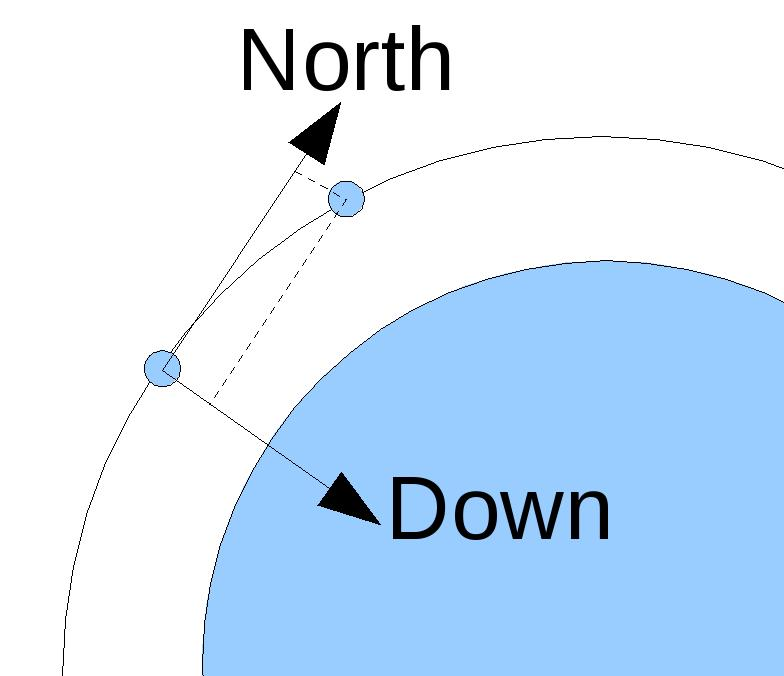
\includegraphics[width=2.5in]{figures/rectilinear.jpg}
\caption{The effect of the curvature of an orbit on the relative state using rectilinear coordinates.}
\label{fig:nedrectilinear}
\end{center}
\end{figure}
















%----------------------------------
\chapter{Product Requirements}\label{ch:NEDreqt}
%----------------------------------


%%%%%%%%%%%%%%%%%%%%%%%%%%%%%%%%%%%%%%%%%%%%%%%%%%%%%%%%%%%%%%%%%%%%%%%%%%%%%%%%%
%
% Purpose:  requirements for the NED model
%
% 
%
%%%%%%%%%%%%%%%%%%%%%%%%%%%%%%%%%%%%%%%%%%%%%%%%%%%%%%%%%%%%%%%%%%%%%%%%%%%%%%%%

% add text here to describe general model requirements
% text is of the form:
\requirement{North-East-Down representation}
\label{reqt:NED}
\begin{description}
  \item[Requirement:]\ \newline
     The North-East-Down Derived State will provide the capability for expressing the state of a vehicle in the North-East-Down oriented reference frame of a planet.
  \item[Rationale:]\ \newline
     Capability from JEOD 1.5.
  \item[Verification:]\ \newline
     Inspection, Test
\end{description}

\requirement{North-East-Down frame generation}
\label{reqt:NED_frame}
\begin{description}
  \item[Requirement:]\ \newline
     The North-East-Down Derived State will provide the capability for generating a reference frame oriented with North, East, and Down, as described in the introduction, through which the state of another vehicle may be expressed.
  \item[Rationale:]\ \newline
     Capability from JEOD 1.5.
  \item[Verification:]\ \newline
     Inspection, Test
\end{description}

\section{Requirements Traceability}

\begin{longtable}[c]{||p{3.5in}|p{3.5in}|}
\caption{Requirements Traceability} \\[6pt]
\hline
{\bf Requirement} & {\bf Inspection and Testing} \\ 
\hline \hline
\endfirsthead
\hline
\endfoot
\caption[]{Requirements Traceability (continued)} \\[6pt]
\hline
{\bf Requirement} & {\bf Inspection and Testing} \\ 
\hline \hline
\endhead
\ref{reqt:NED} - North-East-Down representation &
  Insp.~\ref{test:NED} \\ \hline
\ref{reqt:NED_frame} - North-East-Down frame generation &
  Insp.~\ref{test:NED_frame} \\ \hline

\end{longtable}




%----------------------------------
\chapter{Product Specification}\label{ch:NEDspec}
%----------------------------------

\section{Conceptual Design}
%%%%%%%%%%%%%%%%%%%%%%%%%%%%%%%%%%%%%%%%%%%%%%%%%%%%%%%%%%%%%%%%%%%%%%%%%%%%%%%%%
%
% Purpose:  Conceptual part of Product Spec for the NED model
%
% 
%
%%%%%%%%%%%%%%%%%%%%%%%%%%%%%%%%%%%%%%%%%%%%%%%%%%%%%%%%%%%%%%%%%%%%%%%%%%%%%%%%


%\section{Conceptual Design}
The \NEDDesc\ is used to express the state of a vehicle with respect to a planet-fixed, rotating reference frame in a reference frame oriented with local North, East, and Down directions.  The reference frame is defined by East, parallel to the equator (y-axis); Down, perpendicular to the surface (z-axis); and North (x-axis) completes the right-handed coordinate system.  North is not, in general, aligned with the magnetic field, nor the planetary spin axis.

The calculations associated with representing the state in this way are handled by the North-East-Down subset of the planet-fixed model;  see the \href{file:\JEODHOME/models/utils/planet_fixed/docs/planet_fixed.pdf}{\em Planet-Fixed document}~\cite{dynenv:PLANETFIXED} for details.

%\section{Mathematical Formulations}
%%%%%%%%%%%%%%%%%%%%%%%%%%%%%%%%%%%%%%%%%%%%%%%%%%%%%%%%%%%%%%%%%%%%%%%%%%%%%%%%%
%
% Purpose:  Mathematical Formulation part of Product Spec for the NED model
%
% 
%
%%%%%%%%%%%%%%%%%%%%%%%%%%%%%%%%%%%%%%%%%%%%%%%%%%%%%%%%%%%%%%%%%%%%%%%%%%%%%%%%

\section{Mathematical Formulations}

The \NEDDesc\ contains no independent mathematical formulations; the mathematics utilized by the model is provided by the North-East-Down subset of the planet-fixed model, and by the Reference Frames model;  see the \href{file:\JEODHOME/models/utils/planet_fixed/docs/planet_fixed.pdf}{\em Planet-Fixed} ~\cite{dynenv:PLANETFIXED} and the \href{file:\JEODHOME/models/utils/ref\_frames/docs/ref\_frames.pdf}{\em Reference Frames} ~\cite{dynenv:REFFRAMES} documentation for details.  These documents are also linked as appropriate in the detailed design section of this document.


%\section{Detailed Design}

%%%%%%%%%%%%%%%%%%%%%%%%%%%%%%%%%%%%%%%%%%%%%%%%%%%%%%%%%%%%%%%%%%%%%%%%%%%%%%%%%
%
% Purpose:  Detailed part of Product Spec for the NED model
%
% 
%
%%%%%%%%%%%%%%%%%%%%%%%%%%%%%%%%%%%%%%%%%%%%%%%%%%%%%%%%%%%%%%%%%%%%%%%%%%%%%%%%

\section{Detailed Design}
See the \href{file:refman.pdf}{Reference Manual}\cite{derivedstatebib:ReferenceManual} for a summary of member data and member methods for all classes.  

\subsection{Process Architecture}
The architecture for the \NEDDesc\ is trivial, the \NEDDesc\ methods are largely independent of one another.

\subsection{Functional Design}
This section describes the functional operation of the methods in each class.

The \NEDDesc\ contains only one class:
\begin{itemize}
\classitem{NedDerivedState}
\textref{DerivedState}{ref:DerivedState}

This contains the methods \textit{compute\_ned\_frame}, \textit{set\_use\_alt\_pfix}, \textit{initialize}, and \textit{update}:
\begin{enumerate}

\funcitem{compute\_ned\_frame}
This method utilizes methods from the planet-fixed model, see the \href{file:\JEODHOME/models/utils/planet\_fixed/docs/planet\_fixed.pdf}{\em Planet Fixed} documentation~\cite{dynenv:PLANETFIXED} for details on these methods.

It uses the NorthEastDown methods (from the planet-fixed model) \textit{set\_ned\_trans\_states} and \textit{build\_ned\_orientation} to generate the NED state.  The former, in turn, calls the PlanetFixedPosition method \textit{update\_from\_cart} to convert the Cartesian representation into spherical and elliptical representations.  The latter uses these generated latitude and longitude values to  produce a transformation matrix and corresponding quaternions for going from the planet-fixed reference frame to the NorthEastDown reference frame.

\funcitem{set\_use\_alt\_pfix}
This method sets the flag indicating whether to use the default planet-centered, planet-fixed reference frame associated with the planet or the alternate one, if one is available for the planet.

\funcitem{initialize}
The initialization process comprises the following steps:
\begin{enumerate}
\item{} The generic DerivedState initialization routine is called to establish the naming convention of the reference object (i.e., the planet about which the vehicle is orbiting) and state identifier.
\item{} The DerivedState method \textit{find\_planet} is called (which subsequently calls the  \href{file:\JEODHOME/models/dynamics/dyn_manager/docs/dyn_manager.pdf}{\em Dynamics Manager}~\cite{dynenv:DYNMANAGER}) method of the same name to find a planet by name; that name is stored as \textit{reference\_name}, and is usually assigned in an input file.
\item{} Depending on the value of \textit{use\_alt\_pfix}, the element \textit{pfix\_ptr} is set to either the default planet-fixed reference frame or the alternate planet-fixed reference frame of the planet identified by \textit{reference\_name} and the frame is subscribed.
\item{} The name of the NED state is set as \textit{vehicle\_name.planet\_name.ned}.
\item{} The North-East-Down reference frame is added as a child to the \textit{planet\_centered\_planet\_fixed} frame.
\item{} The North-East-Down frame is registered with the Dynamics manager (optional, user can specify with the \textit{register\_frame} flag, default is true).
\item {} The identified planet is then passed into the initialize method for the PlanetFixedPosition object, \textit{ned\_state} (\textit{ned\_state} is a NorthEastDown state, which inherits from PlanetFixedPosition), which simply records a pointer to the planet just found in the PlanetFixedPosition class (see \href{file:\JEODHOME/models/utils/planet\_fixed/docs/planet\_fixed.pdf}{\em Planet Fixed} documentation~\cite{dynenv:PLANETFIXED}).
\end{enumerate}

\funcitem{update}
This method uses the RefFrame method \textit{compute\_relative\_state} (see \href{file:\JEODHOME/models/utils/ref\_frames/docs/ref\_frames.pdf}{\em Reference Frames} documentation~\cite{dynenv:REFFRAMES}) to calculate the full state of the \textit{subject} in the planet fixed reference frame.  Then, it passes the translational part of that state (i.e. position and velocity) into the \textit{compute\_ned\_frame} method.

\end{enumerate}
\end{itemize}



\chapter{User's Guide}\label{ch:NEDuser}
%----------------------------------
The Analysis section of the User's Guide is intended primarily for
users of pre-existing simulations.  
It contains: 
\begin{itemize}
\item A description of how to modify \NEDDesc\ variables after
the simulation
has compiled, including an in-depth discussion of the input file,
\item An overview of how to interpret (but not edit) the S\_define
file,
\item A sample of some of the typical variables that may be logged.
\end{itemize}


The Integration section of the User's Guide is intended for simulation
developers.
It describes the necessary configuration of the \NEDDesc\
within an
S\_define file, and the creation of standard run directories.  The
latter
component assumes a thorough understanding of the preceding Analysis
section of the user guide.
Where applicable, the user may be directed to selected portions of
Product Specification (Chapter \ref{ch:NEDspec}).

The Extension section of the User's Guide is intended primarily for
developers
needing to extend the capability of the \NEDDesc.  Such users
should have a
thorough understanding of how the model is used in the preceding
Integration section, and of the model
specification (described in Chapter \ref{ch:NEDspec}).


\section{Analysis}
%%%%%%%%%%%%%%%%%%%%%%%%%%%%%%%%%%%%%%%%%%%%%%%%%%%%%%%%%%%%%%%%%%%%%%%%%%%%%%%%%
%
% Purpose:  Analysis part of User's Guide for the NED model
%
% 
%
%%%%%%%%%%%%%%%%%%%%%%%%%%%%%%%%%%%%%%%%%%%%%%%%%%%%%%%%%%%%%%%%%%%%%%%%%%%%%%%%

% \section{Analysis}
\label{sec:neduseranalysis}
It must be reiterated that the \NEDDesc\ does not provide a state for the vehicle with which it is associated, it provides a \textit{reference frame}.  The NedDerivedState does contain a member called \textit{ned\_state}, which contains the state of the reference frame with respect to the parent planet-centered planet-fixed reference frame.  This is identical to the planet-fixed state (PlanetaryDerivedState) of the vehicle with respect to the same planet; it is \textbf{not} the North-East-Down state of the vehicle with respect to the same planet. 

\subsection{Identifying the \NEDDesc}
If the North-East-Down reference frame has been included in the simulation, there will be an instance of \textit{NedDerivedState} located in the S\_define file.  This would typically be found in either the vehicle object (usually if the vehicle is to be described in a North-East-Down sense), or a separate relative-state object (usually if a relative state is to be expressed as such).  There should be an accompanying call to an initialization routine, which takes a reference to the \textit{subject\_body} as one if its inputs, and an accompanying call to an update function.  The essential variables \textit{reference\_name} and \textit{ned\_state.altlatlong\_type} are defined elsewhere, often in the input file.

The North-East-Down reference frame, generated by the \NEDDesc, may also be used to represent the state of another vehicle.  In this case, there will be further inclusion of a RelativeDerivedState instance; see the \textref{RelativeDerivedState User's Guide}{sec:relativeuseranalysis} for details on the implementation of RelativeDerivedState.

Example:
\begin{verbatim}
sim_object{
dynamics/derived_state:    NedDerivedState example_of_ned_state;

(initialization) dynamics/derived_state:
example_of_rel_state_object.example_of_ned_state.initialize (
    Inout DynBody &      subject_body = vehicle_1.dyn_body,
    Inout DynManager &   dyn_manager  = manager_object.dyn_manager);
    
{environment} dynamics/derived_state:
example_of_rel_state_object.example_of_ned_state.update ( )

} example_of_rel_state_object;
\end{verbatim}

Then the input file may have entries comparable to:
\begin{verbatim}
example_of_rel_state_object.example_of_ned_state.reference_name = "Earth";
example_of_rel_state_object.example_of_ned_state.ned_state.altlatlong_type = 
                                                      NorthEastDown::spherical;
\end{verbatim}


\subsection{Editing the \NEDDesc}
The planetary identification, and the planetary surface interpretation (spherical / elliptical) are open to edit by the analyst.

\subsection{Output Data}
The following outputs are available from the \NEDDesc, but once again, these are simply the planetary derived states of the origin of the North-East-Down reference frame.  The strength of the \NEDDesc\ comes in its applicability to a RelativeDerivedState; see the \textref{RelativeDerivedState User's Guide}{sec:relativeuseranalysis} for details on the implementation of RelativeDerivedState.
\begin{verbatim}
example_of_rel_state_object.example_of_ned_state.ned_state.cart_coords[0-2]
example_of_rel_state_object.example_of_ned_state.ned_state.sphere_coords.altitude
example_of_rel_state_object.example_of_ned_state.ned_state.sphere_coords.latitude
example_of_rel_state_object.example_of_ned_state.ned_state.sphere_coords.longitude
example_of_rel_state_object.example_of_ned_state.ned_state.ellip_coords.altitude
example_of_rel_state_object.example_of_ned_state.ned_state.ellip_coords.latitude
example_of_rel_state_object.example_of_ned_state.ned_state.ellip_coords.longitude
\end{verbatim}



%\section{Integration}
%%%%%%%%%%%%%%%%%%%%%%%%%%%%%%%%%%%%%%%%%%%%%%%%%%%%%%%%%%%%%%%%%%%%%%%%%%%%%%%%%
%
% Purpose:  Integration part of User's Guide for the NED model
%
% 
%
%%%%%%%%%%%%%%%%%%%%%%%%%%%%%%%%%%%%%%%%%%%%%%%%%%%%%%%%%%%%%%%%%%%%%%%%%%%%%%%%

 \section{Integration}

Simply including the \NEDDesc\ is straightforward; using it to its full capacity is more challenging.

\subsection{Generating the S\_define}

It should be reiterated that if the desire is simply to express the state of a vehicle with respect to the planet, the NedDerivedState and PlanetaryDerivedState perform the same task.  However, the PlanetaryDerivedState is preferred in this situation, because it does not perform the additional task of generating a reference frame.

The North-East-Down model should be used when the state of a vehicle is desired with respect to some point that is not at the center of the planet, e.g., a launch facility.  Under these circumstances, it becomes necessary to instantiate both a NedDerivedState, and a RelativeDerivedState, with the understanding that the NedDerivedState must be evaluated before the RelativeDerivedState (otherwise the RelativeDerivedState output will be based on an out-of-date orientation of the NED reference frame).

An important consequence of using a RelativeDerivedState to express the relative states of two objects in a North-East-Down reference frame requires the consideration of the class structure of both NedDerivedState and RelativeDerivedState.  There are two types of reference frames in use, BodyRefFrame, and RefFrame.  The BodyRefFrame is associated with a DynBody (a body with dynamic properties), while the RefFrame need not be, it can be associated with some fixed (non-dynamic) body or point.

The North-East-Down reference frame in a NedDerivedState is an instance of a RefFrame, there is no requirement that this be attached to a DynBody.  However, the RelativeDerivedState contains both a BodyRefFrame (\textit{subject\_frame}) and a RefFrame (\textit{target\_frame}); the intention is that the state of a body can be expressed in some other reference frame. Therefore, when generating the relative states, it is \textit{not} possible to use the generated North-East-Down reference frame as the subject frame, it must instead be the target frame.  Then, the vehicle whose state is being expressed must be associated with the subject frame, and the \textit{subject\_frame\_name} and \textit{target\_frame\_name} must be set appropriately.  Then, the \textit{direction\_sense} of the Relative Derived State must be \textit{ComputeSubjectStateinTarget}.

An illustration of this is found in the verification simulations for the North-East-Down model (verif/SIM\_NED).  Here, the relative state instance that expresses the state of vehicle1 (\textit{veh}) with respect to vehicle2 (\textit{veh2}), \textit{veh\_wrt\_veh2}, has:
\begin{verbatim}
subject_frame_name = "vehicle1.composite_body";
target_frame_name = "vehicle2.Earth.ned";
direction_sense = RelativeDerivedState::ComputeSubjectStateinTarget;
\end{verbatim}

Notice also in these simulations that the NedDerivedState is contained within the respective vehicle object, while the RelativeDerivedState is contained within the \textit{rel\_state} object.  This assignment is intentional, though not necessary.  What is necessary is that the state of the two vehicles be evaluated before the relative state, and that the NED reference frame be appropriately oriented, based on the state of its parent vehicle, before the relative state can be expressed in that frame.  Therefore, it was chosen to move the relative state calculations to the end of the S\_define, where they will be processed only after the vehicle and NED reference frames have been processed.  This is recommended procedure.

\subsection{Generating the Input File}
The input file (or Modified Data file) must contain the name of the planet, identified as \textit{reference\_name}, and the identification of whether the North-East-Down reference frame should be based on a spherical (geocentric) or elliptical (geodetic) surface.
\begin{verbatim}
example_of_rel_state_object.example_of_ned_state.reference_name = "Earth";
example_of_rel_state_object.example_of_ned_state.ned_state.altlatlong_type = 
                                                       NorthEastDown::spherical;
\end{verbatim}
or
\begin{verbatim}
example_of_rel_state_object.example_of_ned_state.reference_name = "Earth";
example_of_rel_state_object.example_of_ned_state.ned_state.altlatlong_type = 
                                                     NorthEastDown::elliptical;
\end{verbatim}

The user may specify which planet-centered, planet-fixed reference frame (default or alternate) to use as the basis of the relative state calculations for the North-East-Down reference frame. Note: this only works with Planets that have an alternate reference frame defined.
\begin{verbatim}
example_of_rel_state_object.example_of_ned_state.set_use_alt_pfix(False);

\end{verbatim}
or
\begin{verbatim}
example_of_rel_state_object.example_of_ned_state.set_use_alt_pfix(True);

\end{verbatim}

\subsection{Logging the Data}
See the \textref{Analysis}{sec:neduseranalysis} section for a list of available output data, although again, typically, the desired output results from the relative state implementation of the NED reference frame, rather than from the NED state.  See the \textref{Analysis}{sec:relativeuseranalysis} section for a list of available output data from a RelativeDerivedState.


%\section{Extension}
%%%%%%%%%%%%%%%%%%%%%%%%%%%%%%%%%%%%%%%%%%%%%%%%%%%%%%%%%%%%%%%%%%%%%%%%%%%%%%%%%
%
% Purpose:  Extension part of User's Guide for the NED model
%
% 
%
%%%%%%%%%%%%%%%%%%%%%%%%%%%%%%%%%%%%%%%%%%%%%%%%%%%%%%%%%%%%%%%%%%%%%%%%%%%%%%%%

 \section{Extension}

The \NEDDesc\ is not intended to be extensible.  A potential area for further development may be the addition of a comparable reference frame, such as East-North-Up, but this would be a separate entity, not an extension of the NED reference frame.

%----------------------------------
\chapter{Verification and
Validation}\label{ch:NEDivv}
%----------------------------------

\section{Verification}
%%%%%%%%%%%%%%%%%%%%%%%%%%%%%%%%%%%%%%%%%%%%%%%%%%%%%%%%%%%%%%%%%%%%%%%%%%%%%%%%%
%
% Purpose:  Verification part of V&V for the NED model
%
% 
%
%%%%%%%%%%%%%%%%%%%%%%%%%%%%%%%%%%%%%%%%%%%%%%%%%%%%%%%%%%%%%%%%%%%%%%%%%%%%%%%%

% \section{Verification}

%%% code imported from old template structure
\subsection{Inspection of Modeling Requirements}


\inspection{State Encapsulation}\label{inspect:NED}
 The \NEDDesc\ is capable of outputting data as desired, as demonstrated in simulations located at \textit{derived\_state/verif/SIM\_NED/}, thereby satisfying
 requirement \ref{reqt:NED} at the inspection level.

\inspection{Frame Generation}\label{inspect:NED_frame}
 The \NEDDesc\ is capable of generating a reference frame, as demonstrated in simulations located at \textit{derived\_state/verif/SIM\_NED/}, thereby satisfying
 requirement \ref{reqt:NED_frame} at the inspection level.


\subsection{Verification of Model}

 For testing the \NEDDesc, a simulation of two vehicles was established in which the two vehicles are separated by 1 degree on a common orbital trajectory. Both vehicles generate a North-East-Down reference frame, and the relative state of the other vehicle is calculated for both.

\test{Verification of \NEDDesc\ Output Data for Generic Orbits}\label{test:NED}

\begin{description}
\item{Purpose:}\newline
To demonstrate that the data output by the \NEDDesc\ provides meaningful data.

\item{Requirements:}\newline
Satisfactory conclusion of this test satisfies requirement \ref{reqt:NED}

\item{Procedure:}\newline
The data from the North-East-Down output was compared against that from a Planetary Derived State for an identical orbit.  Polar, inclined, and equatorial orbital characteristics were each tested.

\item{Predictions:}
The state output from this simulation should match that from a Planetary Derived State, which has been verified independently in the \textref{PlanetaryDerivedState Verification Section}{ch:planetaryvv}.

\item{Results:}
There appeared to be no, or negligible, differences between the two states. 
\end{description}



\test{Verification of the reference frame orientation}\label{test:NED_frame}
\begin{description}
\item{Purpose:}\newline
To demonstrate that the reference frame generated by the \NEDDesc\ is oriented along the intended axes.

\item{Requirements:}\newline
Satisfactory conclusion of this test satisfies requirement \ref{reqt:NED_frame}

\item{Procedure:}\newline
The relative state data between the two vehicles was compared against theoretical prediction for consistency for polar, inclined, and equatorial orbital characteristics.

\item{Predictions:}
\begin{enumerate}
 \item {Polar orbit.}  
  \begin{enumerate}
   \item{North.} The lead vehicle should be North of the trailing vehicle while latitude is increasing, and South of the trailing vehicle while the latitude is decreasing.  The transition should be sharp, though not coincident between the two frames; as the vehicles cross the pole, the state of the trailing vehicle in the NED frame associated with the lead vehicle should transition first, resulting in a short time when both vehicles are north (or south) of each other. 
   \item {East.}  The relative states should show zero East component in their respective positions.
   \item {Down.}  Because the NED states are rectilinear, both vehicles should be represented as having a state with a positive down component at all times.  See Figure~\ref{fig:nedrectilinear} for a partial illustration of this counter-intuitive phenomenon.  The behavior is also dependent upon the planetary geometry:
   \begin{itemize}
    \item {Spherical.}  The Down component should be constant, at a value equal to $r - r \cos \Delta \theta$.  For these simulations, this value equates to $1.03 km$. 
    \item {Elliptical.} The Down component should oscillate.  In these simulations, the orbit is approximately circular, whereas the definition of \textit{down} is elliptical.  As the vehicles leave the equator, the trailing vehicle should be significantly further below the leading vehicle than the leading vehicle below the trailing vehicle.  As the vehicles approach the poles, the two values should equalize to $1.03 km$, due to symmetry, then drift apart again heading back to the equator; this time, however, the leading vehicle should have the larger down component.  As the vehicles approach the equator again, the values should again equalize, again due to symmetry.  An exaggerated illustration of this is shown in Figure~\ref{fig:nedellipticalrectilinear}.

\begin{figure}[!ht]
\begin{center}
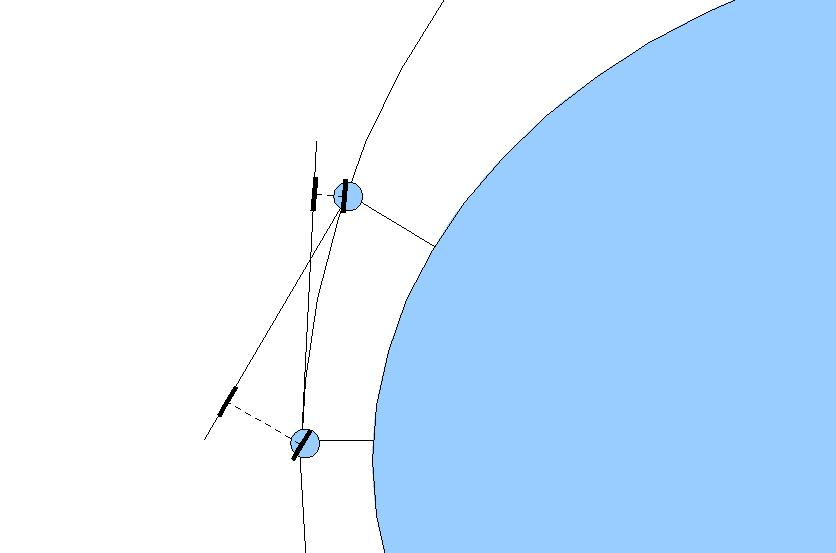
\includegraphics[width=5in]{figures/ned_elliptical_rectilinear.jpg}
\caption{The effect of the difference between the curvature of an orbit and that of the reference ellipse on the relative state using rectilinear coordinates.  The vehicle closer to the equator will exhibit a larger down component in its state than the vehicle farther from the equator.}
\label{fig:nedellipticalrectilinear}
\end{center}
\end{figure}

   \end{itemize}
  \end{enumerate}
 \item {Inclined orbit.}
  \begin{enumerate}
   \item{North.}  As for the polar orbit, the lead vehicle should be North of the trailing vehicle while latitude is increasing, and South of the trailing vehicle while the latitude is decreasing.  Conversely, the transitions at the poles will differ from those observed for the polar orbit; for the inclined orbit, the North component of the relative state should be oscillatory, and ninety degrees out-of-phase from the latitude measurement (so that the North component of the relative state reaches an extremum when the vehicles are at the equator, and goes to zero when the vehicles are at their extreme latitudes).  
   \item {East.}  The lead vehicle should always be East of the trailing vehicle, and the trailing vehicle negative-East of the lead vehicle.
   \item {Down.} By the same argument put forth for the polar orbit, both vehicles should be represented as having a state with a positive down component at all times, constant for spherical geometry and oscillating (though with smaller magnitude due to the variation of the curvature being less significant on an inclined orbit) for the elliptical geometry.  
  \end{enumerate}


 \item {Equatorial orbit.}  
  \begin{enumerate}
   \item{North.} Both relative states should have zero North component.
   \item {East.} The lead vehicle should always be East of the trailing vehicle, and the trailing vehicle negative-East of the lead vehicle.
   \item {Down.} By the same argument put forth for the polar orbit, both vehicles should be represented as having a state with a positive down component at all times, but now be constant for both spherical and elliptical geometries.  
  \end{enumerate}




\end{enumerate}


\item{Results:}
\begin{enumerate}
 \item {Polar orbit.} \ \newline
   The results were mostly as expected.  Figures~\ref{fig:nedpolarell} and \ref{fig:nedpolarellzoom} show the results from the elliptical-geometry reference frame, and Figure~\ref{fig:nedpolarsph} the results from the spherical-geometry reference frame.
  \begin{enumerate}
   \item{North.} The instantaneous switch is seen at polar crossings, with the offset between the two states illustrated better in Figure~\ref{fig:nedpolarellzoom}.  This is at a South pole crossing, and it is clear that the trailing vehicle first transitions to being South of the leading vehicle, then the leading vehicle transitions to being North of the trailing vehicle.
   \item {East.}  The East component is not uniformly zero, it has some instantaneous spikes in its value.  This is attributed to numerical error; those spikes all occur as the vehicles transit the poles, where North and East are not well defined.  
   \item {Down.} For the spherical geometry, the down component shows some oscillation, but that oscillation has magnitude less than $1 cm$, and the mean has the expected value of $1.03 km$.  For the elliptical geometry, the oscillation can clearly be seen.  Figure~\ref{fig:nedpolarellzoom} shows the oscillation from equator heading North (trailing vehicle has larger down component), through the pole at about $1400 s$, then back South to the equator again at approximately $2800 s$.
  \end{enumerate}

\begin{figure}[!ht]
\begin{center}
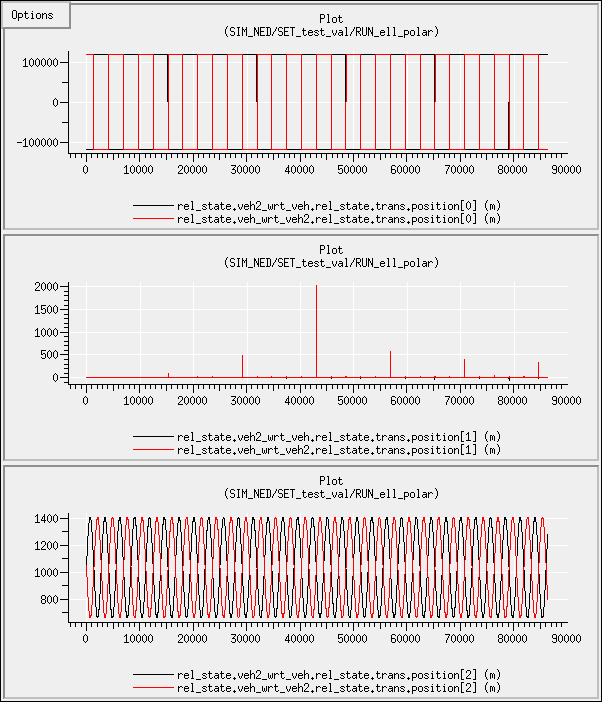
\includegraphics[width=5in]{figures/ned_polar_ell.jpg}
\caption{The relative states for a polar orbit, with elliptical geometry used to define the reference frame.}
\label{fig:nedpolarell}
\end{center}
\end{figure}

\begin{figure}[!ht]
\begin{center}
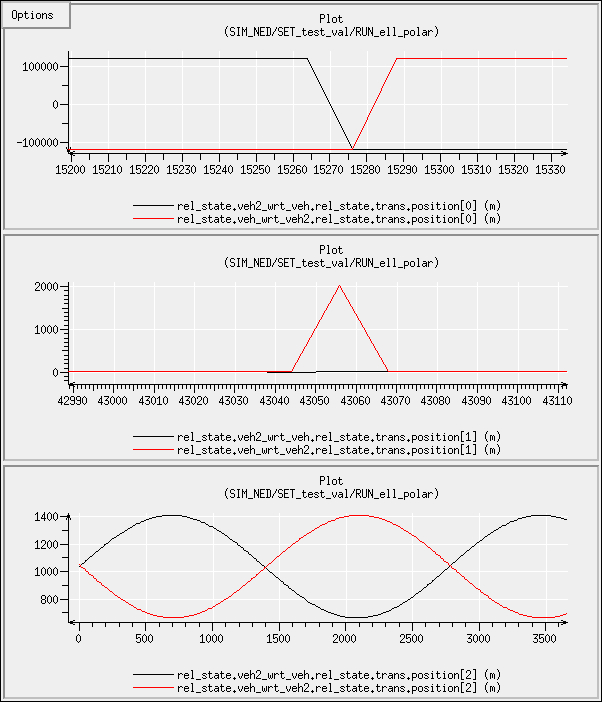
\includegraphics[width=5in]{figures/ned_polar_ell_zoom.jpg}
\caption{The relative states for a polar orbit, with elliptical geometry used to define the reference frame, zoomed in to locations of interest.}
\label{fig:nedpolarellzoom}
\end{center}
\end{figure}

\begin{figure}[!ht]
\begin{center}
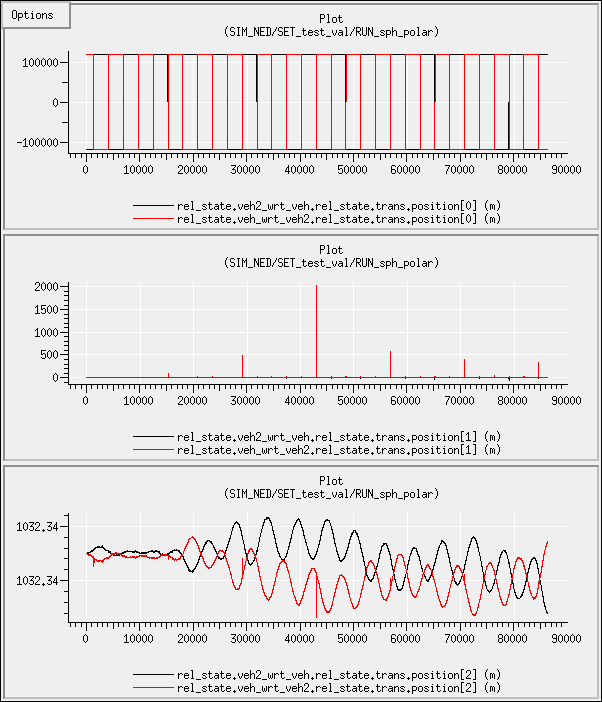
\includegraphics[width=5in]{figures/ned_polar_sph.jpg}
\caption{The relative states for a polar orbit, with spherical geometry used to define the reference frame.}
\label{fig:nedpolarsph}
\end{center}
\end{figure}

\clearpage

\item {Inclined Orbit.} \ \newline
  The results match with expectation.  Figure~\ref{fig:nedincsph} shows the North and East components with the latitude history.  The Down components had a similar oscillation to those seen in the polar orbit and are not shown. A small difference exists of order meters between the North components of the spherical and elliptical geometries, East shows no dependence on geometry, and Down shows a large dependence, as it did in the polar orbit.


\begin{figure}[!ht]
\begin{center}
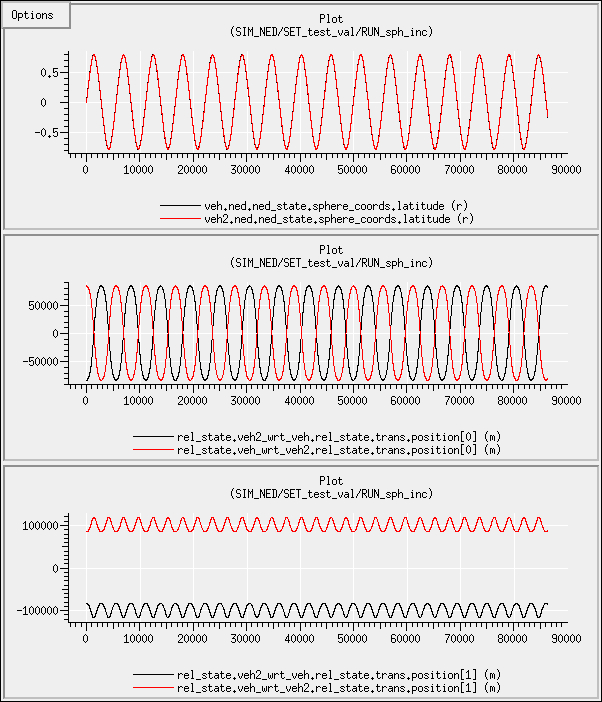
\includegraphics[width=5in]{figures/ned_inc_sph.jpg}
\caption{The variation with time of latitude and of the North and East components of the relative states for an orbit inclined at 45 degrees, with spherical geometry used to define the reference frame.}
\label{fig:nedincsph}
\end{center}
\end{figure}

\clearpage

\item{Equatorial Orbit.}\ \newline
  The results match with expectation.  Figure~\ref{fig:nedequsph} shows the state components; there was no noticeable difference between the spherical and elliptical geometries.
\end{enumerate}

\begin{figure}[!ht]
\begin{center}
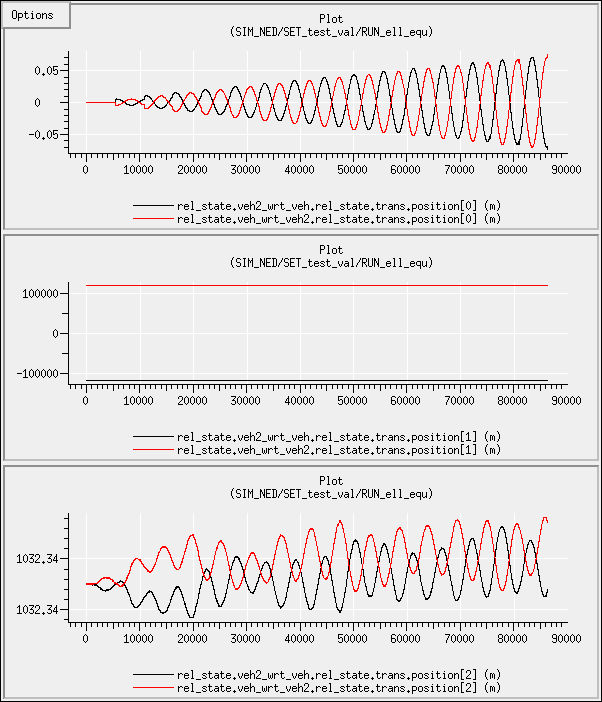
\includegraphics[width=5in]{figures/ned_equ_sph.jpg}
\caption{The relative states for an equatorial orbit with spherical geometry used to define the reference frame.}
\label{fig:nedequsph}
\end{center}
\end{figure}

\end{description}





%\section{Validation}
%%%%%%%%%%%%%%%%%%%%%%%%%%%%%%%%%%%%%%%%%%%%%%%%%%%%%%%%%%%%%%%%%%%%%%%%%%%%%%%%%
%
% Purpose:  Validation part of V&V for the NED model
%
% 
%
%%%%%%%%%%%%%%%%%%%%%%%%%%%%%%%%%%%%%%%%%%%%%%%%%%%%%%%%%%%%%%%%%%%%%%%%%%%%%%%%

\section{Validation}

There is no independent validation of this model.
%%% code imported from old template structure
%\test{<Title>}\label{test:<label>}
%\begin{description}
%\item[Purpose:] \ \newline
%<description>
%\item[Requirements:] \ \newline
%By passing this test, the universal time module 
%partially satisfies requirement~\ref{reqt:<label1>} and 
%completely satisfies requirement~\ref{reqt:<label2>}.
%\item[Procedure:]\ \newline
%<procedure>
%\item[Results:]\ \newline
%<results>
%\end{description}





\part{\OrbElemDescT}



%----------------------------------
\chapter{Introduction}\label{ch:OrbElemintro}
%----------------------------------

\section{Purpose and Objectives of the \OrbElemDescT}
%%%%%%%%%%%%%%%%%%%%%%%%%%%%%%%%%%%%%%%%%%%%%%%%%%%%%%%%%%%%%%%%%%%%%%%%%%%%%%%%%
%
% Purpose:  Introduction for the OrbElem model.
%
% 
%
%%%%%%%%%%%%%%%%%%%%%%%%%%%%%%%%%%%%%%%%%%%%%%%%%%%%%%%%%%%%%%%%%%%%%%%%%%%%%%%%


%\section{Purpose and Objectives of \OrbElemDesc}
% Incorporate the intro paragraph that used to begin this Chapter here. 
% This is location of the true introduction where you explain what this model 
% does.

The \OrbElemDesc\ is used to express the state of a vehicle with respect to the planet about which it is orbiting in terms of its orbital elements:
\begin{itemize}
 \item {Semi-major axis}
\item {Semiparameter, or semi-latus rectum}
\item {Eccentricity}
\item {Inclination}
\item {Argument of periapsis}
\item {Longitude of ascending node}
\item {Anomaly (true, mean, and either eccentric, hyperbolic, or parabolic)}
\item {Mean motion}
\item {Specific orbital energy}
\item {Specific orbital angular momentum}
\end{itemize}

















%----------------------------------
\chapter{Product Requirements}\label{ch:OrbElemreqt}
%----------------------------------


%%%%%%%%%%%%%%%%%%%%%%%%%%%%%%%%%%%%%%%%%%%%%%%%%%%%%%%%%%%%%%%%%%%%%%%%%%%%%%%%%
%
% Purpose:  requirements for the OrbElem model
%
% 
%
%%%%%%%%%%%%%%%%%%%%%%%%%%%%%%%%%%%%%%%%%%%%%%%%%%%%%%%%%%%%%%%%%%%%%%%%%%%%%%%%

% add text here to describe general model requirements
% text is of the form:
\requirement{Cartesian - Orbital Elements conversion}
\label{reqt:OrbElem}
\begin{description}
  \item[Requirement:]\ \newline
    The Orbital Elements Derived State shall provide the capability of outputting data from a cartesian framework as an equivalent set of Keplerian orbital elements.
  \item[Rationale:]\ \newline
     requirement from JEOD 1.5.
  \item[Verification:]\ \newline
     Inspection
\end{description}

\section{Requirements Traceability}

\begin{longtable}[c]{||p{3.5in}|p{3.5in}|}
\caption{Requirements Traceability} \\[6pt]
\hline
{\bf Requirement} & {\bf Inspection and Testing} \\ 
\hline \hline
\endhead
\ref{reqt:OrbElem} - Cartesian - Orbital Elements conversion &
  Insp.~\ref{inspect:OrbElem} \\ \hline


\end{longtable}




%----------------------------------
\chapter{Product Specification}\label{ch:OrbElemspec}
%----------------------------------

\section{Conceptual Design}
%%%%%%%%%%%%%%%%%%%%%%%%%%%%%%%%%%%%%%%%%%%%%%%%%%%%%%%%%%%%%%%%%%%%%%%%%%%%%%%%%
%
% Purpose:  Conceptual part of Product Spec for the OrbElem model
%
% 
%
%%%%%%%%%%%%%%%%%%%%%%%%%%%%%%%%%%%%%%%%%%%%%%%%%%%%%%%%%%%%%%%%%%%%%%%%%%%%%%%%


%\section{Conceptual Design}
The entire process of generating the orbital elements is handled by the Orbital Elements model; see the 
\href{file:\JEODHOME/models/utils/orbital_elements/docs/orbital_elements.pdf}{Orbital Elements document}~\cite{dynenv:ORBITALELEMENTS} for details.


%\section{Mathematical Formulations}
%%%%%%%%%%%%%%%%%%%%%%%%%%%%%%%%%%%%%%%%%%%%%%%%%%%%%%%%%%%%%%%%%%%%%%%%%%%%%%%%%
%
% Purpose:  Mathematical Formulation part of Product Spec for the OrbElem model
%
% 
%
%%%%%%%%%%%%%%%%%%%%%%%%%%%%%%%%%%%%%%%%%%%%%%%%%%%%%%%%%%%%%%%%%%%%%%%%%%%%%%%%

\section{Mathematical Formulations}
The \OrbElemDesc\ has no mathematical formulations, it relies entirely on the Orbital Elements model.
%\section{Detailed Design}

%%%%%%%%%%%%%%%%%%%%%%%%%%%%%%%%%%%%%%%%%%%%%%%%%%%%%%%%%%%%%%%%%%%%%%%%%%%%%%%%%
%
% Purpose:  Detailed part of Product Spec for the OrbElem model
%
% 
%
%%%%%%%%%%%%%%%%%%%%%%%%%%%%%%%%%%%%%%%%%%%%%%%%%%%%%%%%%%%%%%%%%%%%%%%%%%%%%%%%

\section{Detailed Design}
See the \href{file:refman.pdf}{Reference Manual}\cite{derivedstatebib:ReferenceManual} for a summary of member data and member methods for all classes.  

\subsection{Process Architecture}
The architecture for the \OrbElemDesc\ is trivial, comprising few methods that are largely independent.

\subsection{Functional Design}
This section describes the functional operation of the methods in each class.

The \OrbElemDesc\ contains only one class:

\begin{itemize}
\classitem{OrbElemDerivedState}
\textref{DerivedState}{ref:DerivedState}

This contains only the methods \textit{compute\_orbital\_elements}, \textit{initialize} and \textit{update}:
\begin{enumerate}
\funcitem{compute\_orbital\_elements}
Simply calls the Orbital Elements method \textit{from\_cartesian} to convert the data from a Cartesian frame to a set of orbital elements.  See the 
\href{file:\JEODHOME/models/utils/orbital_elements/docs/orbital_elements.pdf}{Orbital Elements document}~\cite{dynenv:ORBITALELEMENTS} for details on this method. 

\funcitem{initialize}
The initialization process comprises the following steps:
\begin{enumerate}
\item{} The generic DerivedState initialization routine is called to assign the \textit{subject} value, establish the naming convention for the state identifier.  
\item{} Calls the Orbital Elements routine \textit{set\_object\_name} to set the name of the vehicle.
\item{} Calls the Derived State method, \textit{find\_planet} to identify the planet with name specified by \textit{reference\_name}.
\item{} Calls the Orbital Elements routine \textit{set\_planet\_name} to set the name of the planet.
\end{enumerate}

\funcitem{update}
Calls the \textit{compute\_orbital\_elements} routine on the planet-relative state.  If the integration frame is planet centered inertial, it uses the basic state of the vehicle.  Otherwise, it calculates the relative state of the vehicle with respect to planet-centered inertial, and uses that as the input to \textit{compute\_orbital\_elements}.


\end{enumerate}
\end{itemize}



\chapter{User's Guide}\label{ch:OrbElemuser}
%----------------------------------
The Analysis section of the User's Guide is intended primarily for
users of pre-existing simulations.  
It contains: 
\begin{itemize}
\item A description of how to modify \OrbElemDesc\ variables after
the simulation
has compiled, including an in-depth discussion of the input file,
\item An overview of how to interpret (but not edit) the S\_define
file,
\item A sample of some of the typical variables that may be logged.
\end{itemize}

The Integration section of the User's Guide is intended for simulation
developers.
It describes the necessary configuration of the \OrbElemDesc\
within an
S\_define file, and the creation of standard run directories.  The
latter
component assumes a thorough understanding of the preceding Analysis
section of the user guide.
Where applicable, the user may be directed to selected portions of
Product Specification (Chapter \ref{ch:OrbElemspec}).

The Extension section of the User's Guide is intended primarily for
developers
needing to extend the capability of the \OrbElemDesc.  Such users
should have a
thorough understanding of how the model is used in the preceding
Integration section, and of the model
specification (described in Chapter \ref{ch:OrbElemspec}).


\section{Analysis}
%%%%%%%%%%%%%%%%%%%%%%%%%%%%%%%%%%%%%%%%%%%%%%%%%%%%%%%%%%%%%%%%%%%%%%%%%%%%%%%%%
%
% Purpose:  Analysis part of User's Guide for the OrbElem model
%
% 
%
%%%%%%%%%%%%%%%%%%%%%%%%%%%%%%%%%%%%%%%%%%%%%%%%%%%%%%%%%%%%%%%%%%%%%%%%%%%%%%%%

% \section{Analysis}
\label{sec:orbelemuseranalysis}

\subsection{Identifying the \OrbElemDescT}
If Orbital Elements have been included in the simulation, there will be an instance of \textit{OrbElemDerivedState} located in the S\_define file.  This would typically be found in either the vehicle object, or a separate relative-state object.  There should be an accompanying call to an initialization routine, which takes a reference to the \textit{subject\_body} as one if its inputs, and an accompanying call to an update function.  The essential \textit{reference\_name} is defined elsewhere, often in the input file.

Example:
\begin{verbatim}
sim_object{
dynamics/derived_state:    OrbElemDerivedState example_of_orb_elem_state;

(initialization) dynamics/derived_state:
example_of_rel_state_object.example_of_orb_elem_state.initialize (
    Inout DynBody &      subject_body = vehicle_1.dyn_body,
    Inout DynManager &   dyn_manager  = manager_object.dyn_manager);
    
{environment} dynamics/derived_state:
example_of_rel_state_object.example_of_orb_elem_state.update ( )

} example_of_rel_state_object;
\end{verbatim}

Then the input file may have entries comparable to:
\begin{verbatim}
example_of_rel_state_object.example_of_orb_elem_state.reference_name = "Earth";
\end{verbatim}


\subsection{Editing the \OrbElemDescT}
There is nothing to edit in the \OrbElemDesc.  The only public data elements are the output data.

\subsection{Output Data}
The various outputs from the \OrbElemDesc, listed in the introduction, are accessible as follows:
\begin{verbatim}
   example_of_rel_state_object.example_of_orb_elem_state.elements.semi_major_axis,
   example_of_rel_state_object.example_of_orb_elem_state.elements.semiparam,
   example_of_rel_state_object.example_of_orb_elem_state.elements.e_mag,
   example_of_rel_state_object.example_of_orb_elem_state.elements.inclination,
   example_of_rel_state_object.example_of_orb_elem_state.elements.arg_periapsis,
   example_of_rel_state_object.example_of_orb_elem_state.elements.long_asc_node,
   example_of_rel_state_object.example_of_orb_elem_state.elements.true_anom,
   example_of_rel_state_object.example_of_orb_elem_state.elements.mean_anom,
   example_of_rel_state_object.example_of_orb_elem_state.elements.orbital_anom,
   example_of_rel_state_object.example_of_orb_elem_state.elements.mean_motion,
   example_of_rel_state_object.example_of_orb_elem_state.elements.orb_energy,
   example_of_rel_state_object.example_of_orb_elem_state.elements.orb_ang_momentum.
\end{verbatim}




%\section{Integration}
%%%%%%%%%%%%%%%%%%%%%%%%%%%%%%%%%%%%%%%%%%%%%%%%%%%%%%%%%%%%%%%%%%%%%%%%%%%%%%%%%
%
% Purpose:  Integration part of User's Guide for the OrbElem model
%
% 
%
%%%%%%%%%%%%%%%%%%%%%%%%%%%%%%%%%%%%%%%%%%%%%%%%%%%%%%%%%%%%%%%%%%%%%%%%%%%%%%%%


 \section{Integration}

Including the \OrbElemDesc\ is relatively straightforward.

 \subsection{Generating the S\_define}

Conventional practice would add the \OrbElemDesc\ to the vehicle object, or (if one exists) to a separate relative-state object at the end of the S\_define file.  When adding the state to a specific vehicle, care must be taken to ensure that the calls to update the state occur after the planet position has been generated from the ephemerides, and the vehicle position integrated.  There is no internal check that this ordering is achieved, the responsibility for ensuring this lies entirely on the Integrator.

The instance of \textit{OrbElemDerivedState} needs to be defined, the model initialized, and a routine update scheduled.  A simple example of how this may look is found in the \textref{Analysis}{sec:orbelemuseranalysis} section.  A simple example simulation is found in the 
\textit{derived\_state/verif/OrbElem} verification simulations released with \JEODid.

\subsection{Generating the Input File}
The input file (or Modified Data file) must contain the name of the planet, identified as \textit{reference\_name}.

The user may specify which inertial reference frame (default or alternate) to use as the basis of the orbital element calculations. Note: this only works with Planets that have an alternate reference frame defined.
\begin{verbatim}
example_of_rel_state_object.example_of_orb_elem_state.set_use_alt_inertial(False);

\end{verbatim}
or
\begin{verbatim}
example_of_rel_state_object.example_of_orb_elem_state.set_use_alt_inertial(True);

\end{verbatim}

See the \textref{Analysis}{sec:orbelemuseranalysis} section for an example of how the input data may appear.

\subsection{Logging the Data}
See the \textref{Analysis}{sec:orbelemuseranalysis} section for a list of available output data.


%\section{Extension}
%%%%%%%%%%%%%%%%%%%%%%%%%%%%%%%%%%%%%%%%%%%%%%%%%%%%%%%%%%%%%%%%%%%%%%%%%%%%%%%%%
%
% Purpose:  Extension part of User's Guide for the OrbElem model
%
% 
%
%%%%%%%%%%%%%%%%%%%%%%%%%%%%%%%%%%%%%%%%%%%%%%%%%%%%%%%%%%%%%%%%%%%%%%%%%%%%%%%%

 \section{Extension}

The \OrbElemDesc\ is not intended to be extended.

%----------------------------------
\chapter{Verification and
Validation}\label{ch:OrbElemivv}
%----------------------------------

\section{Verification}
%%%%%%%%%%%%%%%%%%%%%%%%%%%%%%%%%%%%%%%%%%%%%%%%%%%%%%%%%%%%%%%%%%%%%%%%%%%%%%%%%
%
% Purpose:  Verification part of V&V for the OrbElem model
%
% 
%
%%%%%%%%%%%%%%%%%%%%%%%%%%%%%%%%%%%%%%%%%%%%%%%%%%%%%%%%%%%%%%%%%%%%%%%%%%%%%%%%

% \section{Verification}

%%% code imported from old template structure
\inspection{State Encapsulation}\label{inspect:OrbElem}
 The \OrbElemDesc\ is capable of outputting data as desired, as demonstrated in simulation \textit{derived\_state/verif/OrbElem/SIM\_OrbElem/}, thereby satisfying
 requirement \ref{reqt:OrbElem} at the inspection level.  See the 
\href{file:\JEODHOME/models/utils/orbital_elements/docs/orbital_elements.pdf}{Orbital Elements document}~\cite{dynenv:ORBITALELEMENTS} for verification of the Orbital Elements calculations.



%\section{Validation}
%%%%%%%%%%%%%%%%%%%%%%%%%%%%%%%%%%%%%%%%%%%%%%%%%%%%%%%%%%%%%%%%%%%%%%%%%%%%%%%%%
%
% Purpose:  Validation part of V&V for the OrbElem model
%
% 
%
%%%%%%%%%%%%%%%%%%%%%%%%%%%%%%%%%%%%%%%%%%%%%%%%%%%%%%%%%%%%%%%%%%%%%%%%%%%%%%%%

\section{Validation}

%%% code imported from old template structure
%\test{<Title>}\label{test:<label>}
%\begin{description}
%\item[Purpose:] \ \newline
%<description>
%\item[Requirements:] \ \newline
%By passing this test, the universal time module 
%partially satisfies requirement~\ref{reqt:<label1>} and 
%completely satisfies requirement~\ref{reqt:<label2>}.
%\item[Procedure:]\ \newline
%<procedure>
%\item[Results:]\ \newline
%<results>
%\end{description}

There is no independent validation of the \OrbElemDesc.  See the 
\href{file:\JEODHOME/models/utils/orbital_elements/docs/orbital_elements.pdf}{Orbital Elements document}~\cite{dynenv:ORBITALELEMENTS} for validation of the Orbital elements calculations.

\part{\PlanetaryDescT}



%----------------------------------
\chapter{Introduction}\label{ch:Planetaryintro}
%----------------------------------

\section{Purpose and Objectives of the \PlanetaryDescT}
%%%%%%%%%%%%%%%%%%%%%%%%%%%%%%%%%%%%%%%%%%%%%%%%%%%%%%%%%%%%%%%%%%%%%%%%%%%%%%%%%
%
% Purpose:  Introduction for the Planetary model.
%
% 
%
%%%%%%%%%%%%%%%%%%%%%%%%%%%%%%%%%%%%%%%%%%%%%%%%%%%%%%%%%%%%%%%%%%%%%%%%%%%%%%%%


%\section{Purpose and Objectives of \PlanetaryDesc}
% Incorporate the intro paragraph that used to begin this Chapter here. 
% This is location of the true introduction where you explain what this model 
% does.
\label{ch:planetaryintro}
The \PlanetaryDesc\ provides the state of a vehicle in three different representations:
\begin{itemize}
\item{Cartesian coordinates}\ \newline
 Cartesian coordinates are centered and fixed with the planet
\item{Spherical coordinates}\ \newline
These are centered on the planet, with $\phi$ measured from the Cartesian z-axis, and $\theta$ measured in the Cartesian x-y plane from the Cartesian x-axis toward the Cartesian y-axis.  The position is represented as \textit{latitude} ($\frac{\pi}{2} - \phi$), \textit{longitude} ($\theta$), and \textit{altitude} ($r - r_{equatorial}$).
\item{Elliptical coordinates}\ \newline
These are also centered on the planet, with elliptical longitude and latitude being measured to the point on the reference ellipsoid (surface) that has a normal that passes through the point of interest.  See Figure~\ref{fig:planetaryellipticalspherical} for a graphical distinction between spherical and elliptical coordinates.
\end{itemize}

\begin{figure}[htp]
\begin{center}
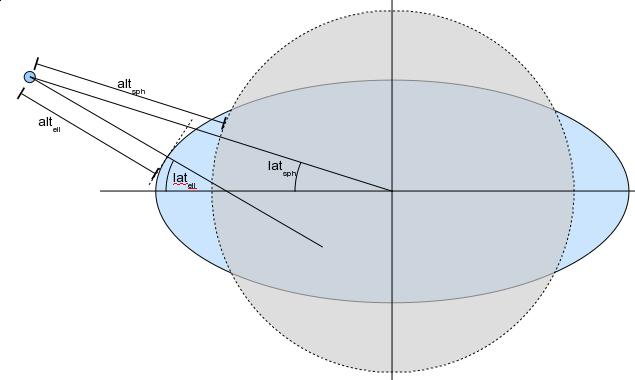
\includegraphics[width=5in]{figures/sphericalelliptical.jpg}
\caption{The differences between spherical and elliptical altitude and latitude.}
\label{fig:planetaryellipticalspherical}
\end{center}
\end{figure}
















%----------------------------------
\chapter{Product Requirements}\label{ch:Planetaryreqt}
%----------------------------------


%%%%%%%%%%%%%%%%%%%%%%%%%%%%%%%%%%%%%%%%%%%%%%%%%%%%%%%%%%%%%%%%%%%%%%%%%%%%%%%%%
%
% Purpose:  requirements for the Planetary model
%
% 
%
%%%%%%%%%%%%%%%%%%%%%%%%%%%%%%%%%%%%%%%%%%%%%%%%%%%%%%%%%%%%%%%%%%%%%%%%%%%%%%%%

% add text here to describe general model requirements
% text is of the form:
\requirement{Planetary representation}
\label{reqt:Planetary}
\begin{description}
  \item[Requirement:]\ \newline
     The Planetary Derived State will provide the capability for expressing the state of one body in a planetary reference frame.
  \item[Rationale:]\ \newline
     Capability from JEOD 1.5.
  \item[Verification:]\ \newline
     Test
\end{description}

\section{Requirements Traceability}

\begin{longtable}[c]{||p{3.5in}|p{3.5in}|}
\caption{Requirements Traceability} \\[6pt]
\hline
{\bf Requirement} & {\bf Inspection and Testing} \\ 
\hline \hline
\endhead
\ref{reqt:Planetary} - Planetary representation &
  Test~\ref{test:Planetary} \\ \hline


\end{longtable}




%----------------------------------
\chapter{Product Specification}\label{ch:Planetaryspec}
%----------------------------------

\section{Conceptual Design}
%%%%%%%%%%%%%%%%%%%%%%%%%%%%%%%%%%%%%%%%%%%%%%%%%%%%%%%%%%%%%%%%%%%%%%%%%%%%%%%%%
%
% Purpose:  Conceptual part of Product Spec for the Planetary model
%
% 
%
%%%%%%%%%%%%%%%%%%%%%%%%%%%%%%%%%%%%%%%%%%%%%%%%%%%%%%%%%%%%%%%%%%%%%%%%%%%%%%%%


%\section{Conceptual Design}

The \PlanetaryDesc\ is used to express the state of a vehicle with respect to a planet-fixed, rotating reference frame.  This is useful, for example, for finding the position of a vehicle with respect to some fixed point on a planetary surface, or for plotting a vehicle trajectory over a map of a planet.

There are three methods for presenting the state, these are described in the \textref{Introduction}{ch:planetaryintro}.
%\section{Mathematical Formulations}
%%%%%%%%%%%%%%%%%%%%%%%%%%%%%%%%%%%%%%%%%%%%%%%%%%%%%%%%%%%%%%%%%%%%%%%%%%%%%%%%%
%
% Purpose:  Mathematical Formulation part of Product Spec for the Planetary model
%
% 
%
%%%%%%%%%%%%%%%%%%%%%%%%%%%%%%%%%%%%%%%%%%%%%%%%%%%%%%%%%%%%%%%%%%%%%%%%%%%%%%%%

\section{Mathematical Formulations}
The mathematical details of the \PlanetaryDesc\ are all handled by other models.  See the Detailed Specification for links.
%\section{Detailed Design}

%%%%%%%%%%%%%%%%%%%%%%%%%%%%%%%%%%%%%%%%%%%%%%%%%%%%%%%%%%%%%%%%%%%%%%%%%%%%%%%%%
%
% Purpose:  Detailed part of Product Spec for the Planetary model
%
% 
%
%%%%%%%%%%%%%%%%%%%%%%%%%%%%%%%%%%%%%%%%%%%%%%%%%%%%%%%%%%%%%%%%%%%%%%%%%%%%%%%%

\section{Detailed Design}
See the \href{file:refman.pdf}{Reference Manual}\cite{derivedstatebib:ReferenceManual} for a summary of member data and member methods for all classes.  

\subsection{Process Architecture}
The architecture for the \PlanetaryDesc\ is trivial, comprising methods that are operationally independent.

\subsection{Functional Design}
This section describes the functional operation of the methods in each class.

The \PlanetaryDesc\ contains only one class:
\begin{itemize}
\classitem{PlanetaryDerivedState}
\textref{DerivedState}{ref:DerivedState}

This contains only the methods \textit{set\_use\_alt\_pfix}, \textit{initialize}, and \textit{update}:
\begin{enumerate}
\funcitem{set\_use\_alt\_pfix}
This method sets the flag indicating whether to use the default planet-centered, planet-fixed reference frame associated with the planet or the alternate one, if one is available for the planet.

\funcitem{initialize}
The initialization process comprises the following steps:
\begin{enumerate}
\item{} The generic DerivedState initialization routine is called to establish the naming convention of the reference object (i.e., the planet about which the vehicle is orbiting) and state identifier.
\item{} The DerivedState method \textit{find\_planet} is called (which subsequently calls the  \href{file:\JEODHOME/models/dynamics/dyn_manager/docs/dyn_manager.pdf}{\em Dynamics Manager}~\cite{dynenv:DYNMANAGER}) method of the same name to find a planet by name; that name is stored as \textit{reference\_name}, and is usually assigned in an input file.
\item{} Depending on the value of \textit{use\_alt\_pfix}, the element \textit{pfix\_ptr} is set to either the default planet-fixed reference frame or the alternate planet-fixed reference frame of the planet identified by \textit{reference\_name} and the frame is subscribed.
\item{} The identified planet is then passed into the initialize method for the PlanetFixedPosition object, \textit{state}, which simply records a pointer to the planet just found in the PlanetFixedPosition class (see \href{file:\JEODHOME/models/utils/planet\_fixed/docs/planet\_fixed.pdf}{\em Planet Fixed} documentation~\cite{dynenv:PLANETFIXED}).
\end{enumerate}

\funcitem{update}
This method uses the RefFrame method \textit{compute\_position\_from} (see \href{file:\JEODHOME/models/utils/ref\_frames/docs/ref\_frames.pdf}{\em Reference Frames} documentation~\cite{dynenv:REFFRAMES}) to calculate the Cartesian position of the \textit{subject} in the planet fixed reference frame.  Then, it uses the PlanetFixedPosition method \textit{update\_from\_cart} 
(see \href{file:\JEODHOME/models/utils/planet\_fixed/docs/planet\_fixed.pdf}{\em Planet Fixed} documentation~\cite{dynenv:PLANETFIXED}) 
to convert the Cartesian representation into spherical and elliptical representations.

\end{enumerate}
\end{itemize}



\chapter{User's Guide}\label{ch:Planetaryuser}
%----------------------------------
The Analysis section of the User's Guide is intended primarily for
users of pre-existing simulations.  
It contains: 
\begin{itemize}
\item A description of how to modify \PlanetaryDesc\ variables after
the simulation
has compiled, including an in-depth discussion of the input file,
\item An overview of how to interpret (but not edit) the S\_define
file,
\item A sample of some of the typical variables that may be logged.
\end{itemize}

The Integration section of the User's Guide is intended for simulation
developers.
It describes the necessary configuration of the \PlanetaryDesc\
within an
S\_define file, and the creation of standard run directories.  The
latter
component assumes a thorough understanding of the preceding Analysis
section of the user guide.
Where applicable, the user may be directed to selected portions of
Product Specification (Chapter \ref{ch:Planetaryspec}).

The Extension section of the User's Guide is intended primarily for
developers
needing to extend the capability of the \PlanetaryDesc.  Such users
should have a
thorough understanding of how the model is used in the preceding
Integration section, and of the model
specification (described in Chapter \ref{ch:Planetaryspec}).


\section{Analysis}
%%%%%%%%%%%%%%%%%%%%%%%%%%%%%%%%%%%%%%%%%%%%%%%%%%%%%%%%%%%%%%%%%%%%%%%%%%%%%%%%%
%
% Purpose:  Analysis part of User's Guide for the Planetary model
%
% 
%
%%%%%%%%%%%%%%%%%%%%%%%%%%%%%%%%%%%%%%%%%%%%%%%%%%%%%%%%%%%%%%%%%%%%%%%%%%%%%%%%

% \section{Analysis}

\label{sec:planetaryuseranalysis}

\subsection{Identifying the \PlanetaryDescT}
If Planet-based states have been included in the simulation, there will be an instance of \textit{PlanetaryDerivedState} located in the S\_define file.  This would typically be found in either the vehicle object, or a separate relative-state object.  There should be an accompanying call to an initialization routine, which takes a reference to the \textit{subject\_body} as one if its inputs, and an accompanying call to an update function.  The \textit{reference\_name} is defined elsewhere, possibly in the input file; this is the name of the planet,with respect to which the state will be evaluated.

Example:
\begin{verbatim}
sim_object{
dynamics/derived_state:    PlanetaryDerivedState example_of_planetary_state;

(initialization) dynamics/derived_state:
example_of_rel_state_object.example_of_planetary_state.initialize (
    Inout DynBody &      subject_body = vehicle_1.dyn_body,
    Inout DynManager &   dyn_manager  = manager_object.dyn_manager);
    
{environment} dynamics/derived_state:
example_of_rel_state_object.example_of_planetary_state.update ( )

} example_of_rel_state_object;
\end{verbatim}

Then the input file may have an entry comparable to:
\begin{verbatim}
example_of_rel_state_object.example_of_planetary_state.reference_name = "Earth";
\end{verbatim}

\subsection{Editing the \PlanetaryDescT}
There is very little to edit in the \PlanetaryDesc, apart from the \textit{reference\_name}, which will result in the planetary state being calculated with respect to a different planet.  It should be noted that \textit{reference\_frame} is only used at initialization, and therefore changing this name \textit{after} the initialization will have no effect.  The \textit{reference\_name} is used to identify the appropriate planet memory location during initialization and thereafter the variable \textit{planet} is used, not \textit{reference\_frame}.

\subsection{Output Data}
The output available from this model is the position of the vehicle with respect to the planet, in planet-fixed coordinates.  This position is available as a Cartesian, spherical, or elliptical coordinate representation.
\begin{verbatim}
example_of_rel_state_object.example_of_planetary_state.state.cart_coords[0-2]
example_of_rel_state_object.example_of_planetary_state.state.sphere_coords.altitude
example_of_rel_state_object.example_of_planetary_state.state.sphere_coords.latitude
example_of_rel_state_object.example_of_planetary_state.state.sphere_coords.longitude
example_of_rel_state_object.example_of_planetary_state.state.ellip_coords.altitude
example_of_rel_state_object.example_of_planetary_state.state.ellip_coords.latitude
example_of_rel_state_object.example_of_planetary_state.state.ellip_coords.longitude
\end{verbatim}

The rotational state is not available.

%\section{Integration}
%%%%%%%%%%%%%%%%%%%%%%%%%%%%%%%%%%%%%%%%%%%%%%%%%%%%%%%%%%%%%%%%%%%%%%%%%%%%%%%%%
%
% Purpose:  Integration part of User's Guide for the Planetary model
%
% 
%
%%%%%%%%%%%%%%%%%%%%%%%%%%%%%%%%%%%%%%%%%%%%%%%%%%%%%%%%%%%%%%%%%%%%%%%%%%%%%%%%

 \section{Integration}

Including the \PlanetaryDesc\ is relatively straightforward.

 \subsection{Generating the S\_define}

Conventional practice would add the \PlanetaryDesc\ to the vehicle object, or (if one exists) to a separate relative-state object at the end of the S\_define file.  When adding the state to a specific vehicle, care must be taken to ensure that the calls to update the state occur after the planet position has been generated from the ephemerides, and the vehicle position integrated.  There is no internal check that this ordering is achieved, the responsibility for ensuring this lies entirely on the Integrator.

The instance of \textit{PlanetaryDerivedState} needs to be defined, the model initialized, and a routine update scheduled.  A simple example of how this may look is found in the \textref{Analysis}{sec:planetaryuseranalysis} section.  Simple example simulations are found in the 
\textit{derived\_state/verif/Planetary} verification simulations released with \JEODid.

\subsection{Generating the Input File}
The input file (or Modified Data file) must contain the name of the planet, identified as \textit{reference\_name}.

In the input file, the user may specify which planet-centered, planet-fixed reference frame (default or alternate) to use as the basis of the position calculations. Note: this only works with Planets that have an alternate reference frame defined.
\begin{verbatim}
example_of_rel_state_object.example_of_planetary_state.set_use_alt_pfix(False);

\end{verbatim}
or
\begin{verbatim}
example_of_rel_state_object.example_of_planetary_state.set_use_alt_pfix(True);

\end{verbatim}

See the \textref{Analysis}{sec:planetaryuseranalysis} section for an example of how the input data may appear.

\subsection{Logging the Data}
See the \textref{Analysis}{sec:planetaryuseranalysis} section for a list of available output data.


%\section{Extension}
%%%%%%%%%%%%%%%%%%%%%%%%%%%%%%%%%%%%%%%%%%%%%%%%%%%%%%%%%%%%%%%%%%%%%%%%%%%%%%%%%
%
% Purpose:  Extension part of User's Guide for the Planetary model
%
% 
%
%%%%%%%%%%%%%%%%%%%%%%%%%%%%%%%%%%%%%%%%%%%%%%%%%%%%%%%%%%%%%%%%%%%%%%%%%%%%%%%%

 \section{Extension}

The \PlanetaryDesc\ is not intended to be extensible.

%----------------------------------
\chapter{Verification and
Validation}\label{ch:Planetaryivv}
%----------------------------------

\section{Verification}
%%%%%%%%%%%%%%%%%%%%%%%%%%%%%%%%%%%%%%%%%%%%%%%%%%%%%%%%%%%%%%%%%%%%%%%%%%%%%%%%%
%
% Purpose:  Verification part of V&V for the Planetary model
%
% 
%
%%%%%%%%%%%%%%%%%%%%%%%%%%%%%%%%%%%%%%%%%%%%%%%%%%%%%%%%%%%%%%%%%%%%%%%%%%%%%%%%

% \section{Verification}

%%% code imported from old template structure
\label{ch:planetaryvv}

\subsection{Inspection of Modeling Requirements}

\inspection{State Encapsulation}\label{inspect:Planetary}
 The \PlanetaryDesc\ is capable of outputting data as desired, thereby satisfying
 requirement \ref{reqt:Planetary} at the inspection level.  The validity of the output data is tested below.


\subsection{Verification of Surface Representations}

\test{Verification of \PlanetaryDesc\ Output Data for Generic Orbits}\label{test:Planetary}

\begin{description}
\item{Purpose:}\newline
To demonstrate that the data output by the \PlanetaryDesc\ provides meaningful data.

\item{Requirements:}\newline
Satisfactory conclusion of this test satisfies requirement \ref{reqt:Planetary}

\item{Procedure:}\newline
A simulation was developed containing an arbitrary vehicle initialized into one of several orbits:
\begin{enumerate}
 \item {Low Earth Orbit, equatorial.}\ \newline  
Initialized with an apo-altitude and peri-altitude of 400 km, and an inclination of zero.
 \item {Low Earth Orbit, inclined.}  \ \newline
Initialized with an apo-altitude and peri-altitude of 400 km, and an inclination of 45 degrees.
 \item {Low Earth Orbit, polar.}\ \newline
  Initialized with an apo-altitude and peri-altitude of 400 km, and an inclination of 90 degrees.
 \item {Eccentric Earth Orbit, equatorial.}\ \newline
  Initialized with an apo-altitude of 8,000 km, a peri-altitude of 400 km, and an inclination of zero.
 \item {Near-Geosynchronous Orbit.}\ \newline
  Initialized with an apo-altitude and peri-altitude of 35,786 km, and an inclination of zero.
\end{enumerate}
The data from the five simulations were compared against theory and against each other. 


\item{Predictions:}
\begin{enumerate}
 \item {Low Earth Orbit, equatorial}
\begin{itemize}
\item{}The Cartesian coordinate output from this data should be close to 0 on the z-axis, and be oscillatory on the x-and y- axes, with a period equal to the synodic period of the satellite, approximately 5,940 seconds.
\item{}The inertial position should oscillate on all three axes with a period equal to the sidereal period of the satellite, approximately 5,560 seconds.
\item{}The altitude should remain approximately constant. The longitude should have a saw-tooth appearance with a variation that is linear with time, rising to $\pi$ radians, and resetting to $-\pi$ radians instantaneously, with a period equal to the synodic period of the satellite. The latitude should remain at zero.
\end{itemize}

\item {Low Earth Orbit, inclined}
\begin{itemize}
\item{}The Cartesian coordinate output from this data should show the same periodic behavior as for the equatorial orbit on the x- and y-axes, with an additional 1-day oscillation in the magnitude of the x- and y- axis magnitudes due to the rotation of Earth underneath the orbit (when the orbital nodes lie close to the x-axis, the x-axis oscillation should be close to the full magnitude of 6,800 km, and the y-axis oscillation only at $6,778 km ~ \sin (\pi / 2) =  4,800 km$, and vice-versa.
On the z-axis, there should be some oscillation with a magnitude of approximately $6,778 km ~ \sin (\pi / 2) =  4,800 km$, and a period equal to the sidereal period of approximately 5,560 seconds.
\item{}The inertial position should show a similar pattern to that for the equatorial orbit, with the same period.
\item{}The altitude should remain approximately constant when expressed in spherical coordinates, but differ significantly when expressed in elliptical (geodetic) coordinates to account for the reduced radius of Earth at higher latitudes.  The difference between the elliptical altitude and spherical altitude should be maximized at high latitudes, and zero at equatorial latitudes.  The period of this oscillation should be the sidereal period of the satellite.
The longitude should exhibit a saw-tooth pattern, but the rise is not expected to be linear; the vehicle will be covering longitude more rapidly at high latitudes than near the equator; while its speed is constant, the vehicle is traveling perpendicular to lines of longitude at high latitudes, but not at equatorial latitudes.  The period of this oscillation should be the synodic period of the satellite.
The latitude should oscillate between $\pm \frac{\pi}{4}$ with a period equal to the sidereal period.
\end{itemize}

\item {Low Earth Orbit, polar}
\begin{itemize}
\item{}The Cartesian coordinate output from this data should continue the trend seen in going to a 45 degree inclination; the z-axis amplitude should increase to the full 6,800 km, and the day-long oscillation on the x-and y-axes should force their respective amplitudes to vary between 0 and the full 6,800 km, ninety degrees out of phase with each other.
\item{}The inertial position should should show a similar pattern to that for the equatorial orbit, with the same period.
\item{}The altitude should show the same pattern as exhibited for the inclined orbit, but with the geodetic altitude reaching a maximum of 21 km above the spherical altitude as the vehicle crosses the poles.
The longitude should show a day-long trend, with a transition at every polar crossing of $\pi$ radians.
The latitude should show a linear triangular oscillation as the latitude varies uniformly while the vehicle heading is northerly and southerly at a constant rate.
\end{itemize}

\item {Eccentric Earth Orbit, equatorial}
\begin{itemize}
\item{}The altitude will vary significantly.  Because of the difference in speed between apoapsis and periapsis, this variation will not be sinusoidal, but should have a steeper gradient near periapsis.  The altitude will oscillate with the sidereal period of the vehicle.
The longitude should exhibit a quasi-sawtooth pattern, but will have significant variation in its gradient due to the varying speed and proximity of the vehicle (when the vehicle is closer, at the same speed, it should cover more longitude in any given time step; when the vehicle is closer, it is also moving faster, exacerbating this feature).  The longitude oscillation will be at the synodic period of the vehicle, whereas the proximity of the vehicle to the planet oscillates at the sidereal period.  Therefore, the ``sawteeth'' are not expected to be equal, the section of the tooth with a steep gradient (vehicle is close to the planet) will gradually migrate across the tooth edge. 
The latitude should remain at zero.  The altitude should oscillate non-sinusoidally, but with constant amplitude on each axis since the orbit is not rotating with respect to the inertial axes (orbital precession is neglected since the orbit is so close to equatorial) 
\item{}The Cartesian coordinate output from this data should exhibit oscillatory-on-oscillatory behavior, as the x- and y-axes rotate on and off the major axis of the orbit.  The oscillation should not be sinusoidal, as observed for the altitude-longitude-latitude plot.
\item{}The inertial position should exhibit non-sinusoidal oscillatory behavior on all three axes, with each axis having constant amplitude over time.  The three axes must not be in phase, and there is no expectation on the relative magnitude of the oscillation from axis to axis.
\end{itemize}

\item {Near-Geosynchronous Orbit.}
\begin{itemize}
\item{}The Cartesian coordinate output from this data should show minimal variation on all three axes; the vehicle should be stationary above a constant point on Earth.
\item{}The inertial position should show one complete oscillation (simulation ran for 24 hours) on all three axes.
\item{}The altitude, latitude, and longitude should all show minimal variation through the simulation.
\end{itemize}

\end{enumerate}

\item{Results:}
\begin{enumerate}
 \item {Low Earth Orbit, equatorial.}
\begin{itemize}
\item{}The Cartesian coordinate gradually diverge from 0 on the z-axis, but by less than 10 meters over a day.  The period of oscillation on the other axes matches that from prediction.  See Figure~\ref{fig:planetaryleoequcart}
\item{}The inertial position oscillates on all three axes with a period equal to that predicted.  See Figure~\ref{fig:planetaryleoequinrtl}
\item{}The altitude remains approximately constant (the variation seen in Figure~\ref{fig:planetaryleoequlal} is less than 1 meter). The longitude exhibits the expected saw-tooth appearance with the correct period. The latitude diverges slowly from zero, but only to less than a micro-radian.  See Figure~\ref{fig:planetaryleoequlal}.
\end{itemize}

\begin{figure}[!ht]
  \begin{center}
        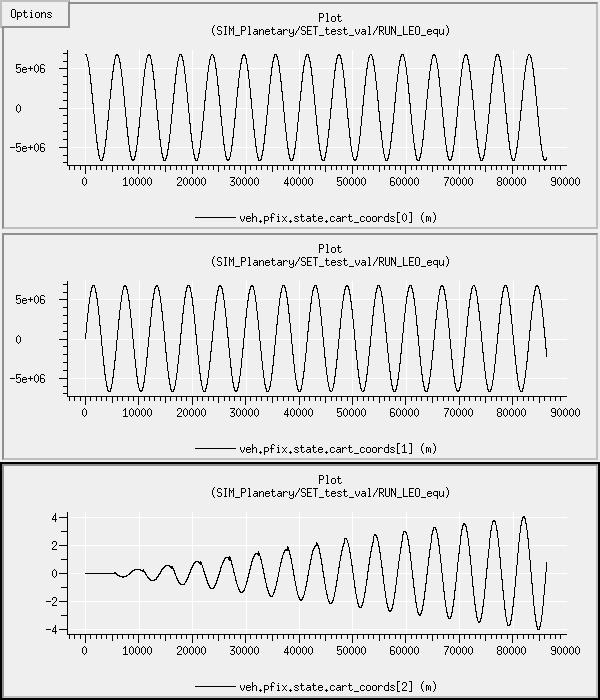
\includegraphics[width=80mm]{figures/planetary_leo_equ_cart.jpg}
        \caption{The variation of position with time, expressed in Cartesian coordinates.} 
        \label{fig:planetaryleoequcart}
  \end{center}
\end{figure}

\begin{figure}[!ht]
  \begin{center}
        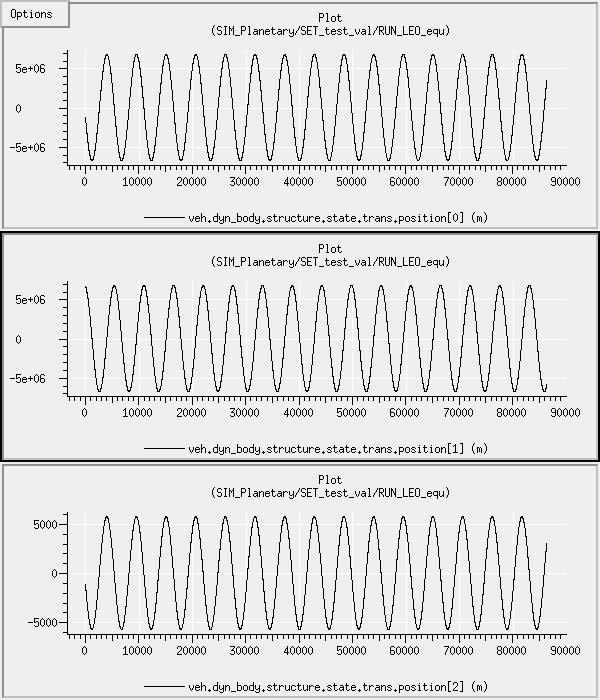
\includegraphics[width=80mm]{figures/planetary_leo_equ_inrtl.jpg}
        \caption{The variation of position with time, expressed in inertial coordinates.} 
        \label{fig:planetaryleoequinrtl}
  \end{center}
\end{figure}

\begin{figure}[!ht]
  \begin{center}
        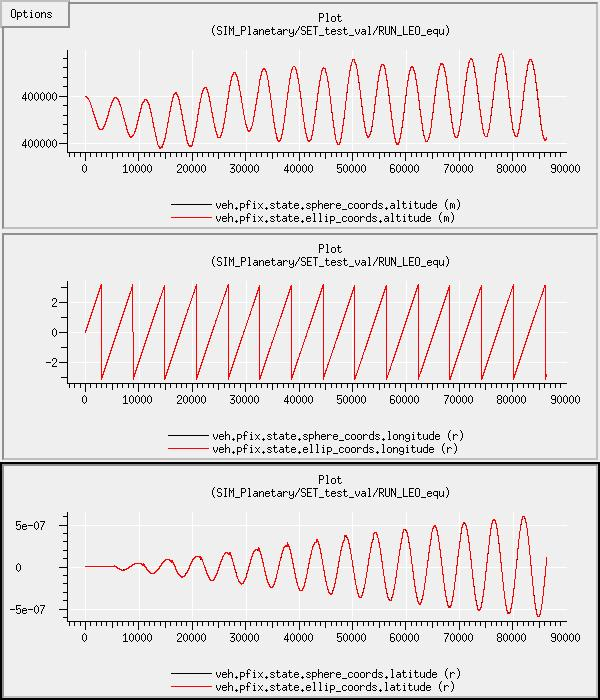
\includegraphics[width=80mm]{figures/planetary_leo_equ_lal.jpg}
        \caption{The variation of position with time, expressed in Altitude-Longitude-Latitude coordinates, both spherical and elliptical (geodetic).} 
        \label{fig:planetaryleoequlal}
  \end{center}
\end{figure}

\clearpage

\item {Low Earth Orbit, inclined.}\ \newline
All data is as expected.  See Figures~\ref{fig:planetaryleoinccart}, \ref{fig:planetaryleoincinrtl}, and~\ref{fig:planetaryleoinclal}.  Figure~\ref{fig:planetaryleoincinrtl} superposes the data from the equatorial low-altitude orbit with that from the inclined low-altitude orbit.

\begin{figure}[!ht]
  \begin{center}
        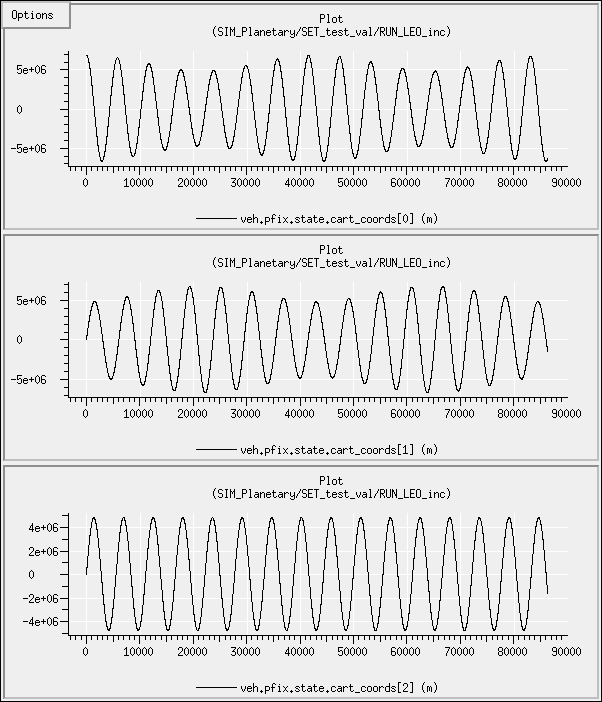
\includegraphics[width=80mm]{figures/planetary_leo_inc_cart.jpg}
        \caption{The variation of position with time, expressed in Cartesian coordinates.} 
        \label{fig:planetaryleoinccart}
  \end{center}
\end{figure}

\begin{figure}[!ht]
  \begin{center}
        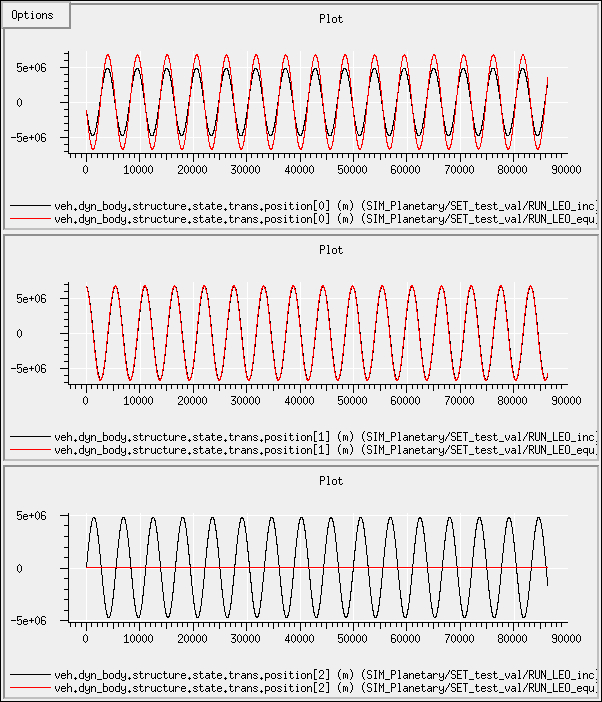
\includegraphics[width=80mm]{figures/planetary_leo_inc_inrtl.jpg}
        \caption{The variation of position with time, expressed in inertial coordinates.} 
        \label{fig:planetaryleoincinrtl}
  \end{center}
\end{figure}

\begin{figure}[!ht]
  \begin{center}
        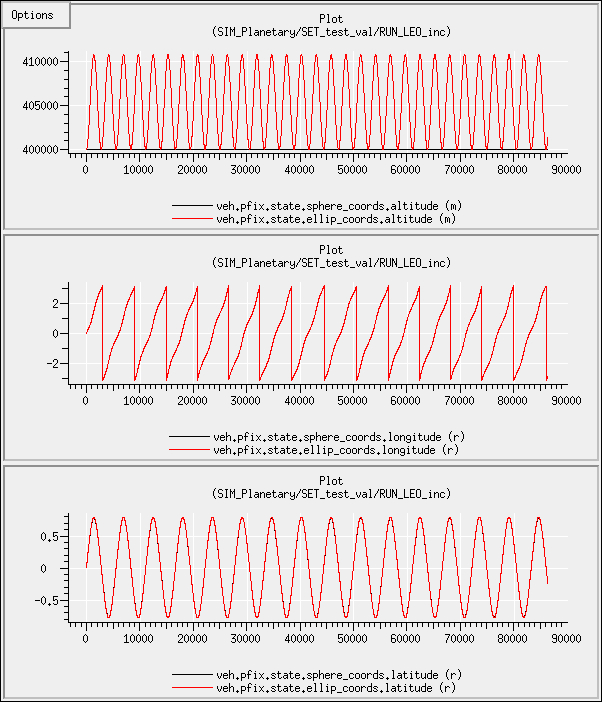
\includegraphics[width=80mm]{figures/planetary_leo_inc_lal.jpg}
        \caption{The variation of position with time, expressed in Altitude-Longitude-Latitude coordinates, both spherical and elliptical (geodetic).} 
        \label{fig:planetaryleoinclal}
  \end{center}
\end{figure}

\clearpage

\item {Low Earth Orbit, polar.}\ \newline
All data is as expected.  See Figures~\ref{fig:planetaryleopolarcart}, \ref{fig:planetaryleopolarinrtl}, and~\ref{fig:planetaryleopolarlal}.  Figure~\ref{fig:planetaryleopolarinrtl} superposes the data from the equatorial low-altitude orbit with that from the inclined low-altitude orbit and the low-altitude polar orbit.

\begin{figure}[!ht]
  \begin{center}
        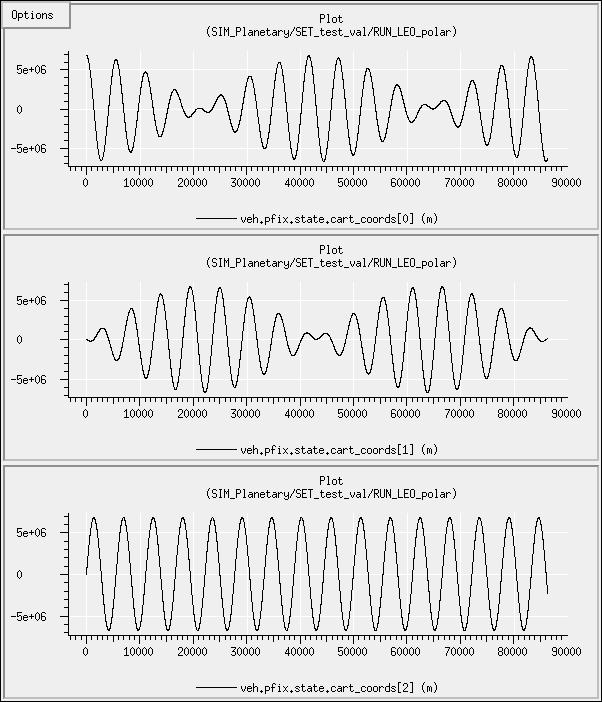
\includegraphics[width=80mm]{figures/planetary_leo_polar_cart.jpg}
        \caption{The variation of position with time, expressed in Cartesian coordinates.} 
        \label{fig:planetaryleopolarcart}
  \end{center}
\end{figure}

\begin{figure}[!ht]
  \begin{center}
        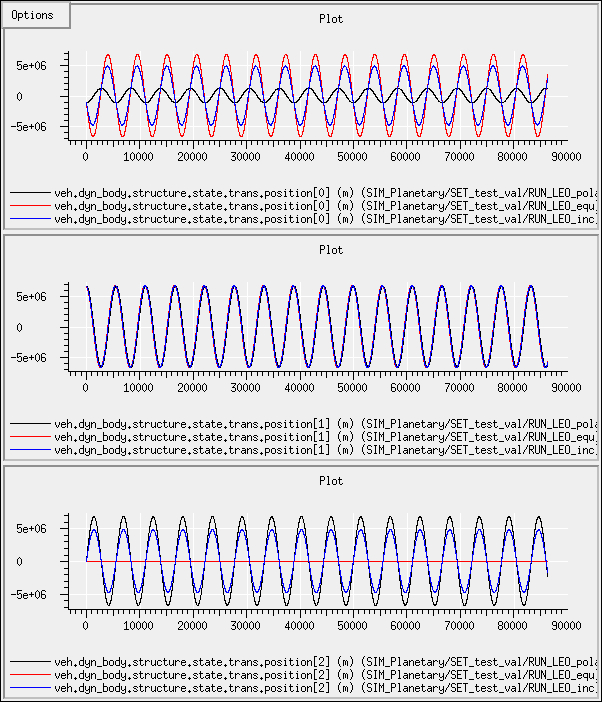
\includegraphics[width=80mm]{figures/planetary_leo_polar_inrtl.jpg}
        \caption{The variation of position with time, expressed in inertial coordinates.} 
        \label{fig:planetaryleopolarinrtl}
  \end{center}
\end{figure}

\begin{figure}[!ht]
  \begin{center}
        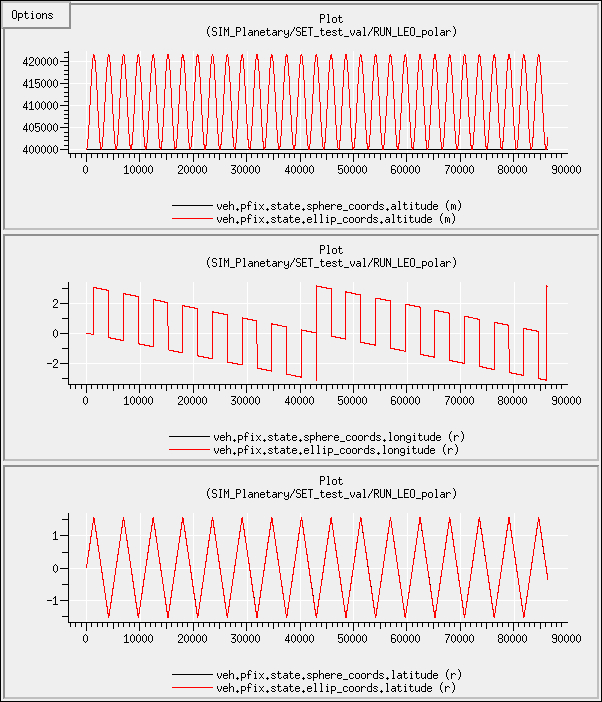
\includegraphics[width=80mm]{figures/planetary_leo_polar_lal.jpg}
        \caption{The variation of position with time, expressed in Altitude-Longitude-Latitude coordinates, both spherical and elliptical (geodetic).} 
        \label{fig:planetaryleopolarlal}
  \end{center}
\end{figure}

\clearpage

\item {Eccentric Earth Orbit, equatorial.}\ \newline
All data is as expected.  See Figures~\ref{fig:planetaryleoecccart}, \ref{fig:planetaryleoeccinrtl}, and~\ref{fig:planetaryleoecclal}.  

\begin{figure}[!ht]
  \begin{center}
        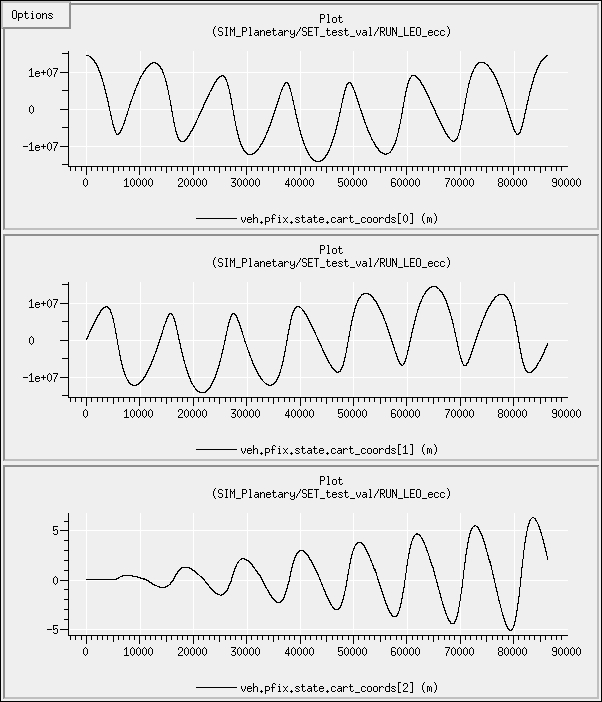
\includegraphics[width=80mm]{figures/planetary_leo_ecc_cart.jpg}
        \caption{The variation of position with time, expressed in Cartesian coordinates.} 
        \label{fig:planetaryleoecccart}
  \end{center}
\end{figure}

\begin{figure}[!ht]
  \begin{center}
        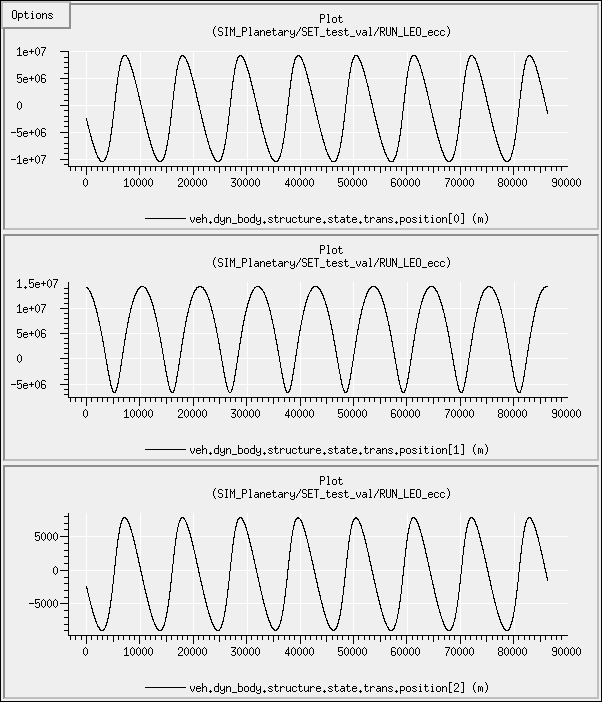
\includegraphics[width=80mm]{figures/planetary_leo_ecc_inrtl.jpg}
        \caption{The variation of position with time, expressed in inertial coordinates.} 
        \label{fig:planetaryleoeccinrtl}
  \end{center}
\end{figure}

\begin{figure}[!ht]
  \begin{center}
        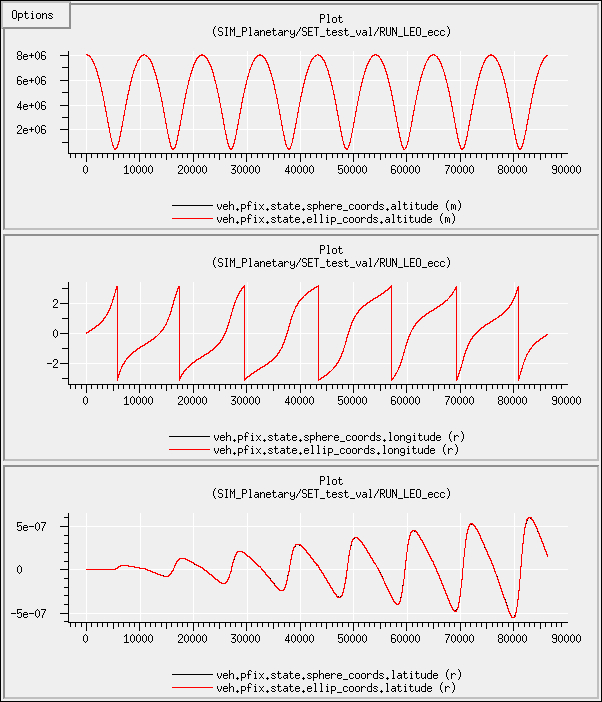
\includegraphics[width=80mm]{figures/planetary_leo_ecc_lal.jpg}
        \caption{The variation of position with time, expressed in Altitude-Longitude-Latitude coordinates, both spherical and elliptical (geodetic).} 
        \label{fig:planetaryleoecclal}
  \end{center}
\end{figure}

\clearpage

\item {Near-Geosynchronous Orbit.}\ \newline
All data is as expected.  See Figures~\ref{fig:planetarygeocart}, \ref{fig:planetarygeoinrtl}, and~\ref{fig:planetarygeolal}.  Note that the variations on the Cartesian and altitude, longitude, latitude values are generally quite small, with the vehicle advancing very slowly along its orbit; this is most likely a result of an altitude that is not quite appropriate for a geosynchronous orbit.
\end{enumerate}

\begin{figure}[!ht]
  \begin{center}
        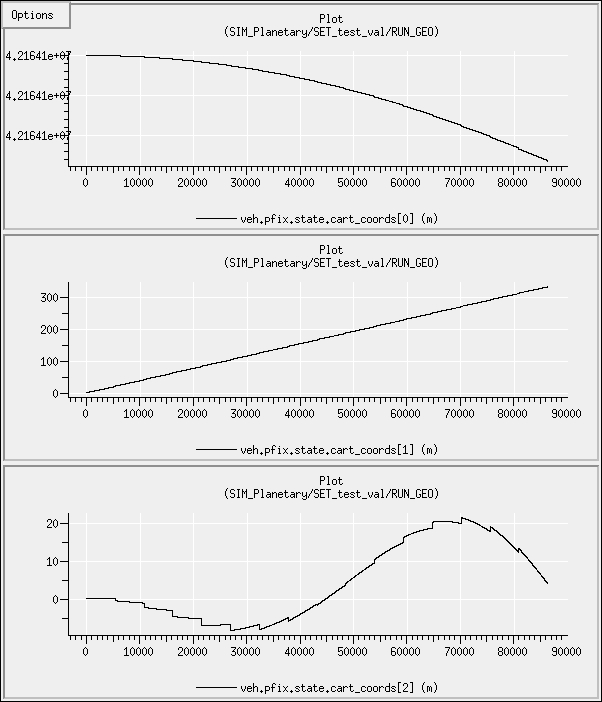
\includegraphics[width=80mm]{figures/planetary_geo_cart.jpg}
        \caption{The variation of position with time, expressed in Cartesian coordinates.} 
        \label{fig:planetarygeocart}
  \end{center}
\end{figure}

\begin{figure}[!ht]
  \begin{center}
        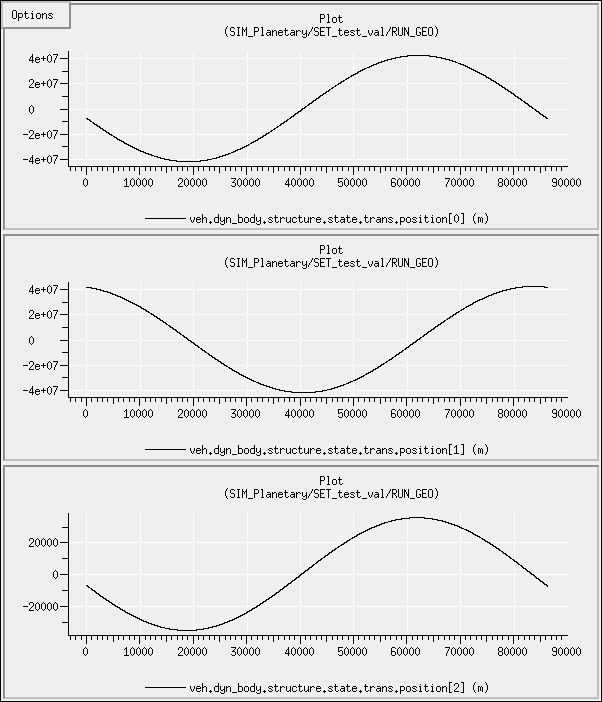
\includegraphics[width=80mm]{figures/planetary_geo_inrtl.jpg}
        \caption{The variation of position with time, expressed in inertial coordinates.} 
        \label{fig:planetarygeoinrtl}
  \end{center}
\end{figure}

\begin{figure}[!ht]
  \begin{center}
        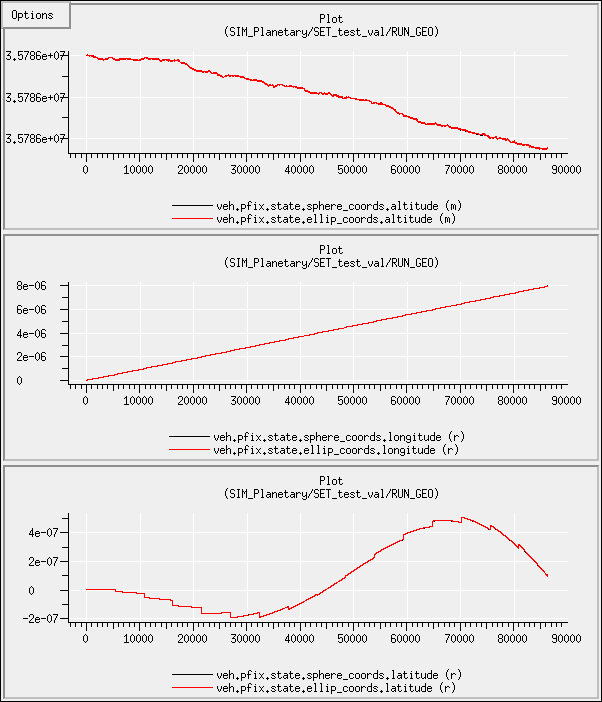
\includegraphics[width=80mm]{figures/planetary_geo_lal.jpg}
        \caption{The variation of position with time, expressed in Altitude-Longitude-Latitude coordinates, both spherical and elliptical (geodetic).} 
        \label{fig:planetarygeolal}
  \end{center}
\end{figure}

\clearpage

\end{description}





%\section{Validation}
%%%%%%%%%%%%%%%%%%%%%%%%%%%%%%%%%%%%%%%%%%%%%%%%%%%%%%%%%%%%%%%%%%%%%%%%%%%%%%%%%
%
% Purpose:  Validation part of V&V for the Planetary model
%
% 
%
%%%%%%%%%%%%%%%%%%%%%%%%%%%%%%%%%%%%%%%%%%%%%%%%%%%%%%%%%%%%%%%%%%%%%%%%%%%%%%%%

\section{Validation}

%%% code imported from old template structure
%\test{<Title>}\label{test:<label>}
%\begin{description}
%\item[Purpose:] \ \newline
%<description>
%\item[Requirements:] \ \newline
%By passing this test, the universal time module 
%partially satisfies requirement~\ref{reqt:<label1>} and 
%completely satisfies requirement~\ref{reqt:<label2>}.
%\item[Procedure:]\ \newline
%<procedure>
%\item[Results:]\ \newline
%<results>
%\end{description}

This method has not been validated against external data.



\part{\RelativeDescT}



%----------------------------------
\chapter{Introduction}\label{ch:Relativeintro}
%----------------------------------

\section{Purpose and Objectives of the \RelativeDescT}
%%%%%%%%%%%%%%%%%%%%%%%%%%%%%%%%%%%%%%%%%%%%%%%%%%%%%%%%%%%%%%%%%%%%%%%%%%%%%%%%%
%
% Purpose:  Introduction for the Relative model.
%
% 
%
%%%%%%%%%%%%%%%%%%%%%%%%%%%%%%%%%%%%%%%%%%%%%%%%%%%%%%%%%%%%%%%%%%%%%%%%%%%%%%%%


%\section{Purpose and Objectives of \RelativeDesc}
% Incorporate the intro paragraph that used to begin this Chapter here. 
% This is location of the true introduction where you explain what this model 
% does.
The \RelativeDesc\ allows the state of one reference frame (e.g. the body reference frame of a vehicle) to be expressed relative to any other reference frame (e.g., the LVLH reference frame of another vehicle). As of JEOD version 3.4, it is no longer required that one of the reference frames be associated with a DynBody; the relative state can now be calculated between any two arbitrary frames in the simulation.

















%----------------------------------
\chapter{Product Requirements}\label{ch:Relativereqt}
%----------------------------------


%%%%%%%%%%%%%%%%%%%%%%%%%%%%%%%%%%%%%%%%%%%%%%%%%%%%%%%%%%%%%%%%%%%%%%%%%%%%%%%%%
%
% Purpose:  requirements for the Relative model
%
% 
%
%%%%%%%%%%%%%%%%%%%%%%%%%%%%%%%%%%%%%%%%%%%%%%%%%%%%%%%%%%%%%%%%%%%%%%%%%%%%%%%%

% add text here to describe general model requirements
% text is of the form:
\requirement{Relative representation}
\label{reqt:Relative}
\begin{description}
  \item[Requirement:]\ \newline
     The Relative Derived State will provide the capability for expressing the state of one reference frame relative to some other reference frame in a specified frame of reference.
  \item[Rationale:]\ \newline
     Capability from JEOD 1.5.
  \item[Verification:]\ \newline
     Inspection, unit test, integrated test by proxy.
\end{description}

\section{Requirements Traceability}

\begin{longtable}[c]{||p{3.5in}|p{3.5in}|}
\caption{Requirements Traceability} \\[6pt]
\hline
{\bf Requirement} & {\bf Inspection and Testing} \\ 
\hline \hline
\endhead
\ref{reqt:Relative} - Relative State Representation &
  Insp.~\ref{inspect:Relative} \\ 
  &
  Test~\ref{test:Relative} \\ \hline

\end{longtable}




%----------------------------------
\chapter{Product Specification}\label{ch:Relativespec}
%----------------------------------

\section{Conceptual Design}
%%%%%%%%%%%%%%%%%%%%%%%%%%%%%%%%%%%%%%%%%%%%%%%%%%%%%%%%%%%%%%%%%%%%%%%%%%%%%%%%%
%
% Purpose:  Conceptual part of Product Spec for the Relative model
%
% 
%
%%%%%%%%%%%%%%%%%%%%%%%%%%%%%%%%%%%%%%%%%%%%%%%%%%%%%%%%%%%%%%%%%%%%%%%%%%%%%%%%


%\section{Conceptual Design}

The \RelativeDesc\ provides the state of one vehicle with respect to some other reference frame (often associated with another vehicle, but not necessarily so).  The two reference frames (the vehicle's reference frame and the other reference frame) are labeled \textit{subject} and \textit{target}.  This model is sufficiently flexible to represent the state of either reference frame with respect to the other.  As of version 3.4, the \textit{subject} frame no longer must be associated with a Dynamic Body, but can be any arbitrary frame in the simulation.  However, the model is fully backwards compatible to the previous usage when it was required to be associated with a Dynamic Body. The \textit{target} never had the Dynamic Body restriction. The original intent was that the subject of the relative state calculation be a vehicle, while the target could be a planet, or some defined point unassociated with any mass, though in actuality the calculation is the same regardless of the nature of the reference frame's owning point or model. The updated capability reflects this.

When expressing the state of some frame, \textit{A} with respect to some other frame, \textit{B}, the tranlational position and velocity are expressed in frame \textit{B}, while the angular velocity is expressed in frame \textit{A}; the angular position (expressed as a quaternion or transformation matrix) is frame-independent.

As a simple example, consider two reference frames, \textit{S} and \textit{S'}.  Suppose that \textit{S'} is moving with some velocity \textit{u} along the x-axis of reference frame \textit{S}, and has its origin momentarily located at $(x_0,y_0)$  Consider further that \textit{S'} is rotated by ninety degrees about the z-axis from \textit{S}, so that $x' = y,  y' = -x, z' = z$.  An illustration is shown in Figure~\ref{fig:relstatereforient}.

\begin{figure}[ht]
\begin{center}
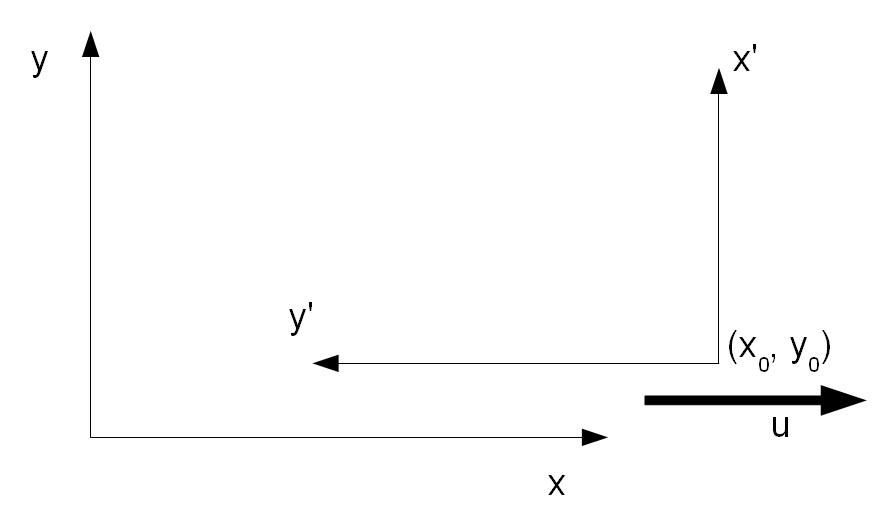
\includegraphics[width=3.5in]{figures/rel_state_ref_orient.jpg}
\caption{The momentary positions, velocity, and orientation of frames \textit{S} and \textit{S'}}
\label{fig:relstatereforient}
\end{center}
\end{figure}

There are four ways of expressing this relation:  the state of \textit{S'} can be expressed with respect to \textit{S}, or \textit{S} with respect to \textit{S'}; for each case, the result could be expressed in \textit{S} or in \textit{S'}.  In this example, the state of  \textit{S'} with respect to \textit{S}, can be represented as 

\begin{align*}
\vec x_{S'|S:S} & = (x_0, y_0) \\ 
\vec v_{S'|S:S} & = (u,0)\\
\vec x_{S'|S:S'} & = (y_0, -x_0) \\
\vec v_{S'|S:S'} & = (0,-u)
\end{align*}

where $ \vec x_{A|B:C}$ is the position of A with respect to B, expressed in C.

Similarly, the state of  \textit{S} with respect to \textit{S'}, can be represented as 

\begin{align*}
\vec x_{S\_S':S} & = (-x_0, -y_0) \\
\vec v_{S\_S':S} & = (-u,0)\\
\vec x_{S\_S':S'} & = (-y_0, x_0)\\
\vec v_{S\_S':S'} & = (0,u)
\end{align*}

Thus, the relative position (or velocity) could be described in four ways, using just these two frames.  Of these four representations, this model can provide $\vec x_{S'|S:S}$ and $\vec x_{S\_S':S'}$.

To make the system completely generic, the usage of \textit{subject} and \textit{target} are, for the most part, just names.  The \RelativeDesc\ will calculate the state of either with respect to the other.  Hence, in the example above, S and S' can be interchangeably identified as \textit{subject} and \textit{target}.  Again, the only restriction on assigning the \textit{subject} and \textit{target} is that the \textit{subject} must be associated with a Dynamic Body.

The user must specify three quantities:
\begin{itemize}
\item{Subject reference frame (by name)}
\item{Target reference frame (by name)}
\item{Sense in which to interpret the request}
\end{itemize}

the latter item in this list can be one of the two values described above:
\begin{itemize}
\item{Subject with respect to Target, expressed in Target (ComputeSubjectStateinTarget)}
\item{Target with respect to Subject, expressed in Subject (ComputeTargetStateinSubject)}
\end{itemize}

Note that this description is intended to convey information on the translational state only.  The angular velocity of the Subject frame will be expressed in the Subject frame, and the angular velocity of the Target frame will be expressed in the target frame.  The expression of the relative orientations of the two frames is frame independent.

%\section{Mathematical Formulations}
%%%%%%%%%%%%%%%%%%%%%%%%%%%%%%%%%%%%%%%%%%%%%%%%%%%%%%%%%%%%%%%%%%%%%%%%%%%%%%%%%
%
% Purpose:  Mathematical Formulation part of Product Spec for the Relative model
%
% 
%
%%%%%%%%%%%%%%%%%%%%%%%%%%%%%%%%%%%%%%%%%%%%%%%%%%%%%%%%%%%%%%%%%%%%%%%%%%%%%%%%

\section{Mathematical Formulations}

The mathematical formulation for calculating the \RelativeDesc\ is entirely incorporated into the Reference Frames model (see \href{file:\JEODHOME/models/utils/ref_frames/docs/ref_frames.pdf}{\em Reference Frames}~\cite{dynenv:REFFRAMES}).
%\section{Detailed Design}

%%%%%%%%%%%%%%%%%%%%%%%%%%%%%%%%%%%%%%%%%%%%%%%%%%%%%%%%%%%%%%%%%%%%%%%%%%%%%%%%%
%
% Purpose:  Detailed part of Product Spec for the Relative model
%
% 
%
%%%%%%%%%%%%%%%%%%%%%%%%%%%%%%%%%%%%%%%%%%%%%%%%%%%%%%%%%%%%%%%%%%%%%%%%%%%%%%%%

\section{Detailed Design}
\label{sec:relativedetail}
See the \href{file:refman.pdf}{Reference Manual}\cite{derivedstatebib:ReferenceManual} for a summary of member data and member methods for all classes.  

\subsection{Process Architecture}
The architecture for the \RelativeDesc\ is trivial, comprising methods that are operationally independent.

\subsection{Functional Design}
This section describes the functional operation of the methods in each class.


The \RelativeDesc\ contains only one class:

\begin{itemize}
\classitem{RelativeDerivedState}
\label{ref:RelativeDerivedState}
\textref{DerivedState}{ref:DerivedState}

This contains only the methods \textit{initialize} and \textit{update}:
\begin{enumerate}
\funcitem{initialize}
The initialization process comprises the following steps:
\begin{enumerate}
\item{} The generic DerivedState initialization routine is called to assign the \textit{subject} value, and establish the naming convention for the state identifier.  Note - this is based on the \textit{subject} name, not on the \textit{target} name.  The user may wish to consider this in determining which object to associate as target, and which to associate as subject.
\item{} Ensures that the \textit{subject\_frame} and \textit{target\_frame} are well-defined.
\item{} The registry of active bodies, maintained by the Dynamics Manager (see \href{file:\JEODHOME/models/dynamics/dyn_manager/docs/dyn_manager.pdf}{\em Dynamics Manager Documentation}~\cite{dynenv:DYNMANAGER}) is updated to ensure that the \textit{target\_frame} is being updated, if necessary.
\end{enumerate}

\funcitem{update}
The variable \textit{direction\_sense} can be set to one of two values:
\begin{enumerate}
\item{ComputeSubjectStateinTarget}
\item{ComputeTargetStateinSubject}
\end{enumerate}

The appropriate call is made to the appropriate reference frame's \textit{calculate\_relative\_state} method, using the other reference frame as an argument (e.g., for ComputeSubjectStateinTarget, we are looking for the state of \textit{subject} with respect to \textit{target}, so the subject-frame's method would be called, using the target frame as an argument).


\end{enumerate}
\end{itemize}





\chapter{User's Guide}\label{ch:Relativeuser}
%----------------------------------
The Analysis section of the User's Guide is intended primarily for
users of pre-existing simulations.  
It contains: 
\begin{itemize}
\item A description of how to modify \RelativeDesc\ variables after
the simulation
has compiled, including an in-depth discussion of the input file,
\item An overview of how to interpret (but not edit) the S\_define
file,
\item A sample of some of the typical variables that may be logged.
\end{itemize}

The Integration section of the User's Guide is intended for simulation
developers.
It describes the necessary configuration of the \RelativeDesc\
within an
S\_define file, and the creation of standard run directories.  The
latter
component assumes a thorough understanding of the preceding Analysis
section of the user guide.
Where applicable, the user may be directed to selected portions of
Product Specification (Chapter \ref{ch:Relativespec}).

The Extension section of the User's Guide is intended primarily for
developers
needing to extend the capability of the \RelativeDesc.  Such users
should have a
thorough understanding of how the model is used in the preceding
Integration section, and of the model
specification (described in Chapter \ref{ch:Relativespec}).


\section{Analysis}
%%%%%%%%%%%%%%%%%%%%%%%%%%%%%%%%%%%%%%%%%%%%%%%%%%%%%%%%%%%%%%%%%%%%%%%%%%%%%%%%%
%
% Purpose:  Analysis part of User's Guide for the Relative model
%
% 
%
%%%%%%%%%%%%%%%%%%%%%%%%%%%%%%%%%%%%%%%%%%%%%%%%%%%%%%%%%%%%%%%%%%%%%%%%%%%%%%%%

% \section{Analysis}

\label{sec:relativeuseranalysis}

\subsection{Identifying the \RelativeDescT}
If Relative States have been included in the simulation, there will be an instance of \textit{RelativeDerivedState} located in the S\_define file.  This would typically be found in either the vehicle object, or a separate relative-state object.  There should be an accompanying call to both an initialization routine and an update function.  The \textit{target\_frame} and \textit{subject\_frame} are defined elsewhere, possibly in the input file.

Example:
\begin{verbatim}
sim_object{
dynamics/derived_state:    RelativeDerivedState example_of_rel_der_state;

(initialization) dynamics/derived_state:
example_of_rel_state_object.example_of_rel_der_state.initialize (
    Inout DynBody &      subject_body = vehicle_1.dyn_body,
    Inout DynManager &   dyn_manager  = manager_object.dyn_manager);
    
{environment} dynamics/derived_state:
example_of_rel_state_object.example_of_rel_der_state.update ( )

} example_of_rel_state_object;
\end{verbatim}

Then the input file may have entries comparable to:
\begin{verbatim}
example_of_rel_state_object.example_of_rel_der_state.subject_frame_name = 
                                                 "vehicle_1.composite_body";
example_of_rel_state_object.example_of_rel_der_state.target_frame_name = 
                                                 "vehicle_2.Earth.lvlh";
example_of_rel_state_object.example_of_rel_der_state.direction_sense = 
                              RelativeDerivedState::ComputeSubjectStateinTarget;
\end{verbatim}

(In this case, the relative state provides the state of \textit{vehicle\_1} in the Earth-based LVLH frame associated with \textit{vehicle\_2}.  Note that there are many variations on this concept, so the analyst should not be surprised if entries are significantly different from this example).

As of JEOD version 3.4, it is no longer required that a relative state be associated with a vehicle object. Thus, it can be used to calculate the state between any two arbitrary frames in the simulation. To use it in this manor, one needs only to invoke the initialization routine that does not take a \textit{subject\_body} as input:

\begin{verbatim}
(initialization) dynamics/derived_state:
example_of_rel_state_object.example_of_rel_der_state.initialize (
    Inout DynManager &   dyn_manager  = manager_object.dyn_manager);
\end{verbatim}

All other usage remains the same.

\subsection{Editing the \RelativeDescT}
There is very little to edit in the \RelativeDesc.  Changing the \textit{direction\_sense} is trivial (see section \textref{Detailed Design}{sec:relativedetail} for options).  Changing the \textit{subject\_frame} and \textit{target\_frame} may produce unintended consequences, and should not be attempted at this level; see the \textref{Integration}{sec:relativeintegration} for details on setting up a relative state calculation.


\subsection{Output Data}
The output available from this model is a complete 12-vector state description.

The translational component of the state is accessible as
\begin{verbatim}
example_of_rel_state_object.example_of_rel_der_state.rel_state.trans.position
example_of_rel_state_object.example_of_rel_der_state.rel_state.trans.velocity
\end{verbatim}
The rotational state can be output as either quaternion or transformation matrix, with velocity as either an angular velocity vector, or an angular velocity magnitude and unit vector.  See the documentation on \textit{RefFrameState} in the \href{file:\JEODHOME/models/utils/ref_frames/docs/ref_frames.pdf}{RefFrame document}~\cite{dynenv:REFFRAMES} for details.


%\section{Integration}
%%%%%%%%%%%%%%%%%%%%%%%%%%%%%%%%%%%%%%%%%%%%%%%%%%%%%%%%%%%%%%%%%%%%%%%%%%%%%%%%%
%
% Purpose:  Integration part of User's Guide for the Relative model
%
% 
%
%%%%%%%%%%%%%%%%%%%%%%%%%%%%%%%%%%%%%%%%%%%%%%%%%%%%%%%%%%%%%%%%%%%%%%%%%%%%%%%%

 \section{Integration}
\label{sec:relativeintegration}

Including the \RelativeDesc\ into the simulation requires some knowledge of other reference frames and derived states.

 \subsection{Generating the S\_define}

Conventional practice would add the \RelativeDesc\ to a separate relative-state object at the end of the S\_define file.  It is also possible to add the relative state to a specific vehicle, but care must be taken to ensure that the target frame has been fully updated before the relative state is called.  For example, if the relative state is to be between two vehicles, \textit{A} and \textit{B} (suppose \textit{A} is the \textit{subject}, and \textit{B} the \textit{target}), then the relative state must be generated after object \textit{B}, and the particular reference frame of interest associated with \textit{B}, are both updated.  A simple solution to this is to either place the relative state calculation at the end of the simulation, or to prioritize the call to update the relative state such that is is processed after that of \textit{B}.  There is no internal check that this ordering is achieved, the responsibility for ensuring this lies entirely on the Integrator.

The instance of \textit{RelativeDerivedState} needs to be defined, the model initialized, and a routine update scheduled.  A simple example of how this may look is found in the \textref{Analysis}{sec:relativeuseranalysis} section.  Simple example simulations are found in the verification simulations for the \textref{\NEDDesc}{ch:NEDivv} and the \textref{\LVLHDesc}{ch:LVLHivv} released with \JEODid.  For more complicated setups, where there are multiple relative states defined, it is strongly recommended that all relative states be put together into one relative state object, and grouped under the Relative Kinematics manager.  This manager handles all of the relative states together after all of the individual frames have been evaluated, and avoids the need to make a separate call from the S\_define for each individual state.  See the \href{file:\JEODHOME/models/dynamics/rel\_kin/docs/rel\_kin.pdf}{Relative Kinematics}~\cite{dynenv:RELKIN} document for details.

\subsection{Generating the Input File}
The input file (or Modified Data file) must contain the names of the \textit{subject\_frame} (\textit{subject\_frame\_name}) and \textit{target\_frame} (\textit{target\_frame\_name}), as well as the \textit{direction\_sense} for each instance of a RelativeDerivedState.  The \textit{subject\_body} is defined elsewhere, as it is passed into the initialization routine from the S\_define.  The \textit{subject\_body} so passed into the initialization routine must include a reference frame with a name that matches the \textit{subject\_frame\_name}, or the initialization routine will fail.  See the \href{file:\JEODHOME/models/utils/ref\_frames/docs/ref\_frames.pdf}{Reference Frames}~\cite{dynenv:REFFRAMES} documentation for more details on the convention for naming the reference frames.

See the \textref{Analysis}{sec:relativeuseranalysis} section for an example of how the input data may appear.

\subsection{Logging the Data}
There are multiple variables available for output, to represent the 12-vector state description.  The most commonly used are the relative position and velocity, which are logged by adding the following lines to the list of logging data:
\begin{verbatim}
"example_of_rel_state_object.example_of_rel_der_state.rel_state.trans.position[0-2]",
"example_of_rel_state_object.example_of_rel_der_state.rel_state.trans.velocity[0-2]",
\end{verbatim}

The rotational state has some flexibility in its representation.  The angular position can be accessed through a quaternion or transformation matrix representation, e.g.
\begin{verbatim}
"example_of_rel_state_object.example_of_rel_der_state.rel_state.rot.T_parent_this[0][0-2]",
"example_of_rel_state_object.example_of_rel_der_state.rel_state.rot.T_parent_this[1][0-2]",
"example_of_rel_state_object.example_of_rel_der_state.rel_state.rot.T_parent_this[2][0-2]",
\end{verbatim}

and the angular rates can be accessed through the angular velocity vector, or with a magnitude and unit vector representation, e.g.
\begin{verbatim}
"example_of_rel_state_object.example_of_rel_der_state.rel_state.rot.ang_vel_this[0-2]",
\end{verbatim}


%\section{Extension}
%%%%%%%%%%%%%%%%%%%%%%%%%%%%%%%%%%%%%%%%%%%%%%%%%%%%%%%%%%%%%%%%%%%%%%%%%%%%%%%%%
%
% Purpose:  Extension part of User's Guide for the Relative model
%
% 
%
%%%%%%%%%%%%%%%%%%%%%%%%%%%%%%%%%%%%%%%%%%%%%%%%%%%%%%%%%%%%%%%%%%%%%%%%%%%%%%%%

 \section{Extension}

The \RelativeDesc\ is not intended to be extensible at this time.  An obvious conceptual extension would be the ability to state the frame used to express the state of frame \textit{A} with respect to frame \textit{B}, as opposed to the current capability which dictates the expression frame (e.g. one could wish to express the relative position of frame \textit{A} with respect to frame \textit{B} in frame \textit{A}, or in a third frame, frame \textit{C}, but neither capability is currently available).  However, great care should be taken if this is attempted, due to the nature of the inherent paradigm of the RefFrameState.

 The \RelativeDesc\ takes advantage of the RefFrameState object to describe the state.  It is assumed that the RefFrameState (of frame \textit{A} relative to frame \textit{B}) has the following interpretations:
 \begin{itemize}
  \item Position: expresssed in frame \textit{B}.
  \item Translational velocity: expresssed in frame \textit{B}.
  \item Rotational velocity: expresssed in frame \textit{A}.
 \end{itemize}
 The RefFrameState contains not only those state elements (if it did, the extension would be a trivial transformation), but also provides the methods to manipulate them.  Changing the paradigm by transforming the output data values will make the output inconsistent with the class that represents it, and will invalidate those methods.  However, the output will still be a RefFrameState, so those invalid methods will still be applicable, however inappropriately;  peculiar and unexpected behavior will likely result.  So, while the \RelativeDesc\ can be easily extended conceptually, the implementation of that extension is far beyond the scope of this document.  The capability to provide these extensions is currently under review for future releases.
 


%----------------------------------
\chapter{Verification and
Validation}\label{ch:Relativeivv}
%----------------------------------

\section{Verification}
%%%%%%%%%%%%%%%%%%%%%%%%%%%%%%%%%%%%%%%%%%%%%%%%%%%%%%%%%%%%%%%%%%%%%%%%%%%%%%%%%
%
% Purpose:  Verification part of V&V for the Relative model
%
% 
%
%%%%%%%%%%%%%%%%%%%%%%%%%%%%%%%%%%%%%%%%%%%%%%%%%%%%%%%%%%%%%%%%%%%%%%%%%%%%%%%%

% \section{Verification}

%%% code imported from old template structure
\subsection{Inspection of Behavior in Integrated Testing}
\inspection{Inspection of LVLH and NED Verification Simulations}\label{inspect:Relative}
  The verification of the integrated behavior of the \RelativeDesc\ is performed by proxy in the verification of the \textref{\NEDDesc}{ch:NEDivv} and \textref{\LVLHDesc}{ch:LVLHivv}.  The performance of the simulations in these verification tests indicates that the \RelativeDesc\ is performing as expected at a crude, conceptual level (comparison against analytical results was not performed in this case). This result partially satisfies requirement~\ref{reqt:Relative}.  Requirement~\ref{reqt:Relative} is fully satisfied with the demonstration of performance against analytical results; this demonstration is provided in Test~\ref{test:Relative}. 


\subsection{Analytical Verification of Comprehensive Behavior in Unit Testing}

\test{Analytical Verification of \RelativeDescT\ Output Data for Multiple Scenarios}\label{test:Relative}

\begin{description}
\item[Purpose:]
To demonstrate that the data output by the \RelativeDesc\ provides accurate relative state information in simple, analytical  situations.

\item[Requirements:]
Satisfactory conclusion of this test partially satisfies requirement~\ref{reqt:Relative}.  Requirement~\ref{reqt:Relative} is fully satisfied with the additional demonstration of satisfactory performance within integrated testing; this demonstration is conducted at Inspection~\ref{inspect:Relative}.

\item[Procedure:]
A simulation was developed containing two vehicles in empty space.  Each vehicle
contained one vehicle-point.  Tests were run with the vehicles initialized in
various relative states, and the relative states between the points were
examined.  The state outputs were provided as the relative state of:
\begin{itemize}
 \item A with respect to B, expressed in reference frame B
 \item B with respect to A, expressed in reference frame A
\end{itemize}

\textbf{Notation:}
\begin{itemize}
\item 
Vectors are expressed numerically as a set of three values enclosed in square braces ($[x,y,z]$).
Subscripts on a vector denote the reference frame in which the values are expressed (i.e. which x,y,z axes are being used).
The subscripts used in this section are:
\begin{itemize}
 \item I - inertial
 \item SA - structural of vehicle A
 \item SB - structural of vehicle B
 \item PA - point frame of vehicle A
 \item PB - point frame of vehicle B 
\end{itemize}
\item Position, velocity and angular velocity are symbolically represented by:
\begin{itemize}
 \item $\vec x$ Position.
 \item $\vec v$ Translational velocity.
 \item $\vec \omega$ Rotational velocity.
\end{itemize}
\item Subscripts on the symbolic vector values are to be interpreted as follows ($P$, $Q$, and $R$ are used here as representatives of the frames used in this section):
\begin{itemize}
 \item $\vec x_{P}$ Position of frame $P$ (reference taken from context).
 \item $\vec x_{P|Q}$ Position of frame $P$ with respect to frame $Q$ (expression frame taken from context).
 \item $\vec x_{P|Q:R}$ Position of frame $P$ with respect to frame $Q$, expressed in frame $R$.
\end{itemize}
\item Conventionally,
\begin{itemize}
 \item $\vec x_{P|Q}$ is expressed in frame Q.
 \item $\vec v_{P|Q}$ is expressed in frame Q.
 \item $\vec \omega_{P|Q}$ is expressed in frame P.
\end{itemize}
\end{itemize}



The vehicles were configured as shown in Figure~\ref{fig:Relative_config}.  For
both vehicles, the respective structure and body frames are equivalent; the body frame will 
therefore not be mentioned again in this section.  

Vehicle B
is initially located such that $\vec x_{SB|I} = [0,0,0]_I$, with frame \textit{SB} aligned
with frame \textit{I}.  


Point B (the vehicle point on Vehicle B) is located at \newline
$\vec x_{PB|SB} = [1,0,0]_{SB}$ (initial conditions, $\vec x_{PB|I} = [1,0,0]_I$).
Frame \textit{PB} is initially rotated by -90 degrees
 about the z-axis with respect to frame \textit{SB}.

 Vehicle A is initially located such that $\vec x_{SA|I} = [10, 0, 0]_I$.  Its structural
 reference frame (\textit{SA}) is oriented with a +90 degree rotation about the z-axis from
 frame \textit{I}.  
 
 Frame \textit{PA}, associated with Point A,
 is located such that $\vec x_{PA|SA} = [1, 0, 0]_{SA}$ (initial conditions, $\vec x_{PA|I} =[10,1,0]_I$).
 It has a +90 degree rotation about the z-axis with respect to frame \textit{SA}.

 The dynamic states, where applicable, of the two vehicles are initialized such that:
 \begin{itemize}
   \item $\vec v_{SA|I} = [2 , 1 , 0 ]_I = [-2 , -1 , 0]_{PA}$
   \item $\vec \omega_{SA|I} = [0 , 9 , 0]_{SA}\ deg\ s^{-1} = [-9 ,
   0 , 0]_I\ deg\ s^{-1} = [9 , 0 , 0]_PA\ deg\ s^{-1}$
   \item $\vec v_{SB|I} = [0 , 0 , 1]_I$
   \item $\vec \omega_{SB|I} = [0 , 0 , 4.5]_I\ deg\ s^{-1}$ (same value in frames I,
   SB, PB).
 \end{itemize}

\begin{figure}[!ht]
 \begin{center}
  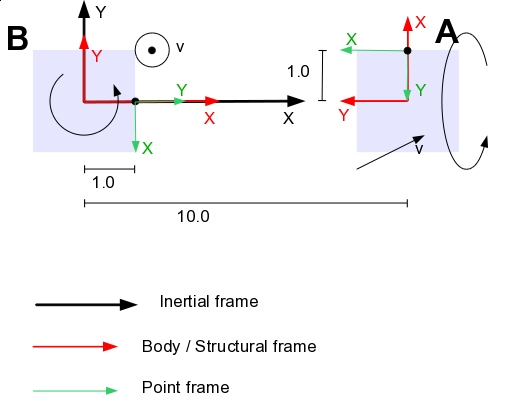
\includegraphics[width=80mm]{figures/relative_config.png}
  \caption{The configuration of the two vehicles and their respective reference frames.} 
  \label{fig:Relative_config}
 \end{center}
\end{figure}


Several simulation setups were considered, gradually increasing in complexity.

First, the rotational states were turned off, and only the effects of 
relative translational motion studied -- first one at a time, then both moving
together.
Then, the translational motion was zeroed, and only the effect of
relative rotational motion considered -- first one at a time, then both
together.
Finally, the situation in which both vehicles had translational and rotational
motion was considered.

\begin{enumerate}
 \item RUN\_no\_rot\_A\_trans
 \item RUN\_no\_rot\_B\_trans
 \item RUN\_no\_rot\_AB\_trans
 \item RUN\_A\_rot\_no\_trans 
 \item RUN\_B\_rot\_no\_trans
 \item RUN\_AB\_rot\_no\_trans  
 \item RUN\_AB\_rot\_AB\_trans  
\end{enumerate}

\item[Predictions:]



\begin{enumerate}
 \item RUN\_no\_rot\_A\_trans \newline
   With no rotation, the relative states are straightforward.  In this case, only vehicle A is moving.
   \begin{itemize}
    \item $\vec x_{PA|PB} = [(-1 - t), (9 + 2t) , 0]_{PB}$
    \item $\vec v_{PA|PB} = [-1 , 2 , 0]_{PB}$
    \item $\vec \omega_{PA|PB} = [0 , 0 , 0]_{PA}$
    \item $\vec x_{PB|PA} = [(9 + 2t) , (1 + t) , 0]_{PA}$
    \item $\vec v_{PB|PA} = [2 , 1 , 0]_{PA}$
    \item $\vec \omega_{PB|PA} = [0 , 0 , 0]_{PB}$
   \end{itemize}

 \item RUN\_no\_rot\_B\_trans \newline
 In this run, vehicle A is static, and vehicle B is moving.
 \begin{itemize}
    \item $\vec x_{PA|PB} = [-1 , 9 , -t]_{PB}$
    \item $\vec v_{PA|PB} = [0 , 0 , -1]_{PB}$
    \item $\vec \omega_{PA|PB} = [0 , 0 , 0]_{PA}$
    \item $\vec x_{PB|PA} = [9 , 1 , t]_{PA}$
    \item $\vec v_{PB|PA} = [0 , 0 , 1]_{PA}$
    \item $\vec \omega_{PB|PA} = [0 , 0 , 0]_{PB}$
   \end{itemize}
 \item RUN\_no\_rot\_AB\_trans \newline
 In this run, both vehicles have translational motion.
   \begin{itemize}
    \item $\vec x_{PA|PB} = [(-1 - t) , (9 + 2t) , -t]_{PB}$
    \item $\vec v_{PA|PB} = [-1 , 2 , -1]_{PB}$
    \item $\vec \omega_{PA|PB} = [0 , 0 , 0]_{PA}$
    \item $\vec x_{PB|PA} = [(9 + 2t) , (1 + t) , t]_{PA}$
    \item $\vec v_{PB|PA} = [2 , 1 , 1]_{PA}$
    \item $\vec \omega_{PB|PA} = [0 , 0 , 0]_{PB}$
   \end{itemize}
 \item RUN\_A\_rot\_no\_trans \newline
  In this run, vehicle A is rotating (bit has no translational motion).  Vehicle B is static.
  
  The motion of A with respect to B, expressed in B, is fairly
  straightforward.  On the y-axis, there is no motion.  On the x-axis, the
  motion starts at zero, and increases as A rotates around towards +x, and
  should follow a sine curve.  On
  the z-axis, the motion starts at a (negative) maximum, and slows, as in a
  negative cosine curve.
  
  In frame A, it is quite apparent that the x-value of the position of
  Point B (i.e. frame B) remains constant, at 9.0.  However, the motion of
  Point B on the y- and z- axes is less obvious.  Point B will clearly be moving
  relative to Point A in the inertial frame, but frame A is rotating at the
  same time.
  
  At any given time, the location of Point A with respect to the center of
  mass of vehicle A is $\vec x_{PA|SA} = [0, -1, 0]_{PA}$, since the y- and z-axes rotate with
  the vehicle.  Point B does not move relative to the vehicle center of
  mass, so must be at $\vec x_{PB|PA} = (9, 1, 0)_{PA}$ relative to frame A.  In other words,
  Point B DOES NOT MOVE in frame \textit{PA}.
       
  This can be illustrated by considering the relative position of \textit{PB} with respect to \textit{PA} in the inertial frame:
  \begin{equation*}
  \begin{split}
    \vec x_{PB|PA} &= [1\ ,\ 0\ ,\ 0]_I - [10\ ,\ \cos k_A t\ ,\ -\sin k_A t]_{I} \\
                 & = [-9\ ,\ -\cos k_A t\ ,\ \sin k_A t]_{I}
  \end{split}
  \end{equation*}

  where $k_A = \frac{2 \pi}{40}\ s^{-1} = 0.157\ s^{-1}$.
  
  With a rotation rate of 9 degrees per second, the rotation period is 40 seconds; there should be 2.5 rotations during the 100 second simulation).
   
     
  The transformation matrix from $I$ to $PA$ is a combination of a 180-degree z=rotation to begin, followed by a dynamic rotation on the x-axis:
  \begin{equation}
   \begin{split}
  T_{I\rightarrow PA} &=\begin{bmatrix} 1 & 0 & 0 \\ 0 & \cos k_A t & \sin k_A t \\  0 & -\sin k_A t & \cos k_A t \end{bmatrix}
  \begin{bmatrix} -1 & 0 & 0 \\ 0 & -1 & 0 \\ 0 & 0 & 1\end{bmatrix} \\
  &= 
  \begin{bmatrix} -1 & 0 & 0 \\ 0 & -\cos k_A t & \sin k_A t \\  0 & \sin k_A t & \cos k_A t \end{bmatrix}
  \end{split}
 \end{equation}\label{eqn:rel_verif_TIPA}

   Hence, applying the transformation matrix to the inertial expression yields:
   \begin{equation*}
   \begin{split}
        \vec x_{PB|PA} &= [9\ ,\ -\cos^2 k_A t -\sin^2 k_A t\ ,\ 0]_{PA} \\
                     &= [9\ ,\ 1\ ,\ 0]_{PA}
   \end{split}
   \end{equation*}

    \begin{itemize}
    \item $\vec x_{PA|PB} = [-\cos k_A t\ ,\ 9\ ,\ -\sin k_A t]_{PB}$
    \item $\vec v_{PA|PB} = [k_A \sin k_A t\ ,\ 0\ ,\ -k_A \cos k_A t]_{PB}$
    \item $\vec \omega_{PA|PB} = [9\ ,\ 0\ ,\ 0]_{PA}\ deg\ s^{-1}$
    \item $\vec x_{PB|PA} = [9\ ,\ 1\ ,\ 0]_{PA}$
    \item $\vec v_{PB|PA} = [0\ ,\ 0\ ,\ 0]_{PA}$
    \item $\vec \omega_{PB|PA} = [0\ ,\ 9\ ,\ 0]_{PB}\ deg\ s^{-1}$
   \end{itemize}

 \item RUN\_B\_rot\_no\_trans \newline
 In this scenario, vehicle B is rotating, and vehicle A is static.  The rotation axis of the rotating vehicle does not pass through the other vehicle's reference point, so the results are a little different to those from the previous test.
 
 The position and velocity of B with respect to A is easier, since the A frame is static.  For position, the x-value will oscillate between 9 and 11, starting at 9;  the y-value will oscillate between 0 and 2, starting at 1 and decreasing;  the z-value remains at 0 throughout.  For velocity:  the x-value starts at 0 and increases initially; the y-value starts at a minimum; z remains 0 throughout.  The angular velocity is a simple rotation on the z-axis.
 
 The position and velocity of A with respect to B is more challenging.  We start by considering the relative position in the inertial frame:
 \begin{equation*}
  \vec x_{PA|PB} = [10 - \cos k_B t\ ,\ 1 - \sin k_B t\ ,\ 0]_{I}
 \end{equation*}
 
 where $k_B = \frac{2 \pi}{80}\ s^{-1} = 0.0785\ s^{-1}$


 The transformation matrix from $I$ to $PB$ is a simple z-axis rotation matrix, since both the initial rotation and the dynamic rotation are on the z-axis:
  \begin{equation}
  T_{I\rightarrow PB} =\begin{bmatrix} \sin k_B t & -\cos k_B t & 0 \\ \cos k_B t & \sin k_B t & 0 \\ 0 & 0 & 1 \end{bmatrix}
 \end{equation}\label{eqn:rel_verif_TIPB}
 
 Hence,
 \begin{equation*}
  \vec x_{PA|PB} = [10 sin k_B t - cos k_B t , 10 cos k_B t + sin k_B t - 1 , 0]_{PB}
 \end{equation*}
 
 The velocity is the derivative of this expression.
 \begin{itemize}
    \item $\vec x_{PA|PB} = [10 \sin k_B t - \cos k_B t\ ,\ 10 \cos k_B t + \sin k_B t - 1\ ,\ 0]_{PB}$
    \item $\vec v_{PA|PB} = [10 k_B \cos k_B t + k_B \sin k_B t\ ,\ k_B \cos k_B t - 10 k_B \sin k_B t\ ,\ 0]_{PB}$
    \item $\vec \omega_{PA|PB} = [0\ ,\ 0\ ,\ -4.5]_{PA}\ deg\ s^{-1}$
    \item $\vec x_{PB|PA} = [10 - \cos k_B t\ ,\ 1 - \sin k_B t\ ,\ 0]_{PA}$
    \item $\vec v_{PB|PA} = [k_B \sin k_B t\ ,\ - k_B \cos k_B t\ ,\ 0]_{PA}$
    \item $\vec \omega_{PB|PA} = [0\ ,\ 0\ ,\ 4.5]_{PB}\ deg\ s^{-1}$
   \end{itemize}
   
   
 \item RUN\_AB\_rot\_no\_trans  \newline
 Combining the two rotations produces:
 \begin{equation*}
 \begin{split}
  \vec x_{PA|PB} &= [10\                   ,\ \cos k_A t\              ,\ -\sin k_A t]_{I} - 
                  [ \cos k_B t\         ,\  \sin k_B t\            ,\ 0]_{I} \\ 
               &=[10 - \cos k_B t\       ,\ \cos k_A t - \sin k_B t\ , -\sin k_A t]_{I}
 \end{split}
 \end{equation*}
 
 and, by symmetry,
 \begin{equation*}
  \vec x_{PB|PA} = - \vec x_{PA|PB}
 \end{equation*}
 
 Applying the transformation matrices (equations~\ref{eqn:rel_verif_TIPA} and~\ref{eqn:rel_verif_TIPB}) provides the relative positions in the appropriate frames.
  
  The translational velocity expressions are derived from the derivatives of the relative positions.
  The rotational velocity expressions are derived in a similar way to the translational positions.
  \begin{equation*}
  \begin{split}
  \vec \omega_{PA|PB} &= [-9\ ,\ 0\    ,\ 0]_{I} \ deg\ s^{-1}- 
                      [0\  ,\ 0\    ,\ 4.5]_{I}\ deg\ s^{-1} \\
                    &=[-9\ ,\ 0\    , -4.5]_{I}\ deg\ s^{-1}
  \end{split}
 \end{equation*}
  \begin{itemize}
    \item $\vec x_{PA|PB} = \begin{bmatrix} 10 \sin k_B t - \cos k_A t \cdot \cos k_B t \\
                                          10 \cos k_B t + \cos k_A t \cdot \sin k_B t - 1 \\ 
                                          -\sin k_A t
                          \end{bmatrix}
                          _{PB}$
 
    \item $\vec v_{PA|PB} = \begin{bmatrix} 
           10 k_B \cdot \cos k_B t + k_B \cdot \cos k_A t \cdot \sin k_B t + k_A \cdot \sin k_A t \cdot \cos k_B t\\
          -10 k_B \cdot \sin k_B t + k_B \cdot \cos k_A t \cdot \cos k_B t - k_A \cdot \sin k_A t \cdot \sin k_B t\\ 
            - k_A \cos k_A t
           \end{bmatrix}_{PB}$
    
    \item $\vec \omega_{PA|PB} = \begin{bmatrix} 9\\
                                               -4.5 sin k_A t\\
                                               -4.5 cos k_A t
                               \end{bmatrix}_{PA}\ deg\ s^{-1}$
    
    \item $\vec x_{PB|PA} = \begin{bmatrix} 10 - \cos k_B t\\
                                          1 - \cos k_A t \cdot \sin k_B t\\
                                          sin k_A t \cdot sin k_B t
                          \end{bmatrix}_{PA}$

    \item $\vec v_{PB|PA} = \begin{bmatrix} 
              k_B \sin k_B t \\
              k_A \cdot \sin k_A t \cdot \sin k_B t - k_B \cdot \cos k_A t \cdot \cos k_B t\\
              k_A \cdot \cos k_A t \cdot \sin k_B t + k_B \cdot \sin k_A t \cdot \cos k_B t\\ 
           \end{bmatrix}_{PA}$
           
    \item $\vec \omega_{PB|PA} = \begin{bmatrix} 9 \sin k_B t\\
                                               9 \cos k_B t\\
                                               4.5 
                               \end{bmatrix}_{PB}\ deg\ s^{-1}$
   \end{itemize}
  
 \item RUN\_AB\_rot\_AB\_trans  \newline
 With this run, the previously generated translational motion is added to the rotational motion; the same methods are applied (i.e. generate inertial expressions, transform to appropriate frame) to obtain the following expressions:
  \begin{itemize}
    \item $\vec x_{PA|PB} = \begin{bmatrix} 10 \sin k_B t - \cos k_A t \cdot \cos k_B t + t(2 \sin k_B t - \cos k_B t)\\
                                          10 \cos k_B t + \cos k_A t \cdot \sin k_B t - 1 + t(2 \cos k_B t + \sin k_B t \\ 
                                          -\sin k_A t - t
                          \end{bmatrix}
                          _{PB}$
 
    \item $\vec v_{PA|PB} = \begin{bmatrix} 
           \cos k_B t ( k_B (10+2t) + k_A (\sin k_A t) -1 )  + \sin k_B t (k_B(t + \cos k_A t) + 2) \\
           \cos k_B t (k_B(t + \cos k_A t) + 2) - \sin k_B t ( k_B (10+2t) + k_A (\sin k_A t) -1 )  \\ 
            - k_A \cos k_A t -1
           \end{bmatrix}_{PB}$
    
    \item $\vec \omega_{PA|PB} = \begin{bmatrix} 9\\
                                               -4.5 sin k_A t\\
                                               -4.5 cos k_A t
                               \end{bmatrix}_{PA}\ deg\ s^{-1}$
    
    \item $\vec x_{PB|PA} = \begin{bmatrix} 10 - \cos k_B t + 2t\\
                                          1 - \cos k_A t \cdot \sin k_B t + t (\cos k_A t + \sin k_A t)\\
                                          sin k_A t \cdot sin k_B t + t (\cos k_A t - \sin k_A t)
                          \end{bmatrix}_{PA}$

    \item $\vec v_{PB|PA} = \begin{bmatrix} 
              k_B \sin k_B t +2 \\
              \sin k_A t (k_A (\sin k_B t - t) +1) + \cos k_A t (1 + k_A t - k_B cos k_B t)\\
              \cos k_A t (k_A (\sin k_B t - t) +1) - \sin k_A t (1 + k_A t - k_B cos k_B t)\\ 
           \end{bmatrix}_{PA}$
           
    \item $\vec \omega_{PB|PA} = \begin{bmatrix} 9 \sin k_B t\\
                                               9 \cos k_B t\\
                                               4.5 
                               \end{bmatrix}_{PB}\ deg\ s^{-1}$
   \end{itemize}
\end{enumerate}

\item[Results:]
For test cases 1-4, the analytical solution is so simple that a simple inspection demonstrated that the results matched the predictions.  Test cases 5-7 required a little more analysis.  The results for test cases 6 and 7 are included below.  The results for test 5 were very similar.
 
 \begin{itemize}
  \item Test Case 6 \newline
  Figures~\ref{fig:rel6_1}-\ref{fig:rel6_4} show the differences between the analytical results and the numerical results for the two relative positions and the relative velocities.
   
   The results show very close agreement between the two sets of data.

 \item Test Case 7 \newline
  Figures~\ref{fig:rel7_1}-\ref{fig:rel7_6} show the differences between the analytical results and the numerical results for the two relative positions, velocities, and angular velocities.
   
   The results show very close agreement between the two sets of data.
  \end{itemize}
  
\item[Conclusion:]
In all cases, the numerical values very closely approximated the analytical values.  This test has demonstrated that the \RelativeDesc\ is correctly calculating the relative states when used in isolation.

In order to demonstrate that the model works identically regardless of whether or not it is associated with a Dynamic Body, an additional relative state was added to each of the test cases described above. It was identical in every way, in every scenario, to one of the already existing relative states, with the exception that it was initialized independently of any Dynamic Body. The generalized results proved to be a bitwise match to those for the pre-existing analog, and thus the results are not separately presented here.
  
 \begin{figure}[!ht]
  \begin{center}
        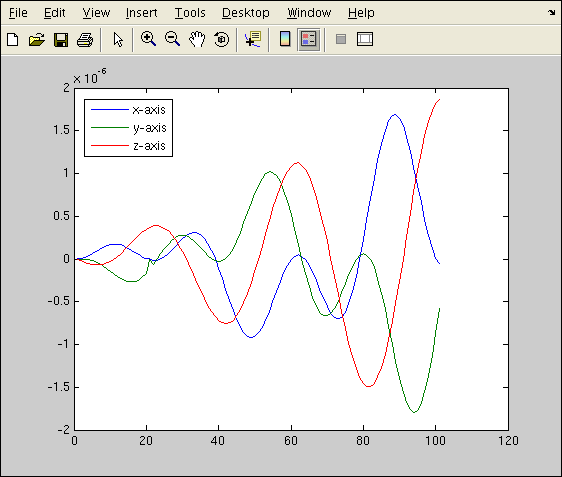
\includegraphics[width=80mm]{figures/relative6_xab.png}
        \caption{The variation with time of the difference between the analytical and numerical solutions for the position of A with respect to B.}
        \label{fig:rel6_1}
  \end{center}
\end{figure}

 \begin{figure}[!ht]
  \begin{center}
        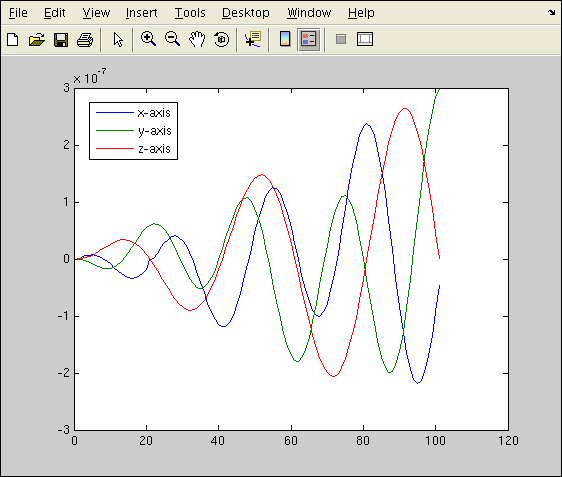
\includegraphics[width=80mm]{figures/relative6_vab.png}
        \caption{The variation with time of the difference between the analytical and numerical solutions for the velocity of A with respect to B.} 
  \end{center}
\end{figure}

 \begin{figure}[!ht]
  \begin{center}
        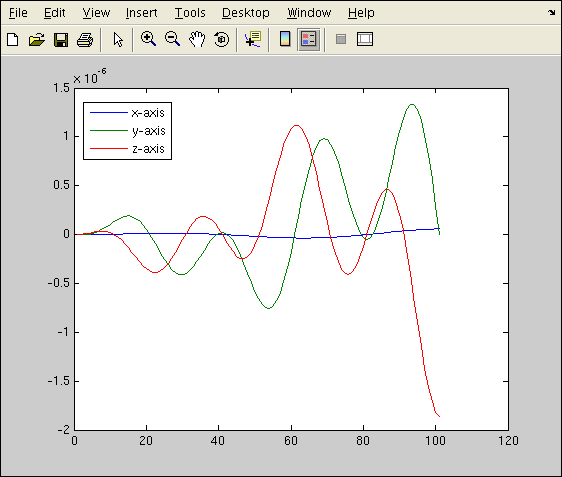
\includegraphics[width=80mm]{figures/relative6_xba.png}
        \caption{The variation with time of the difference between the analytical and numerical solutions for the position of B with respect to A.} 
  \end{center}
\end{figure}

 \begin{figure}[!ht]
  \begin{center}
        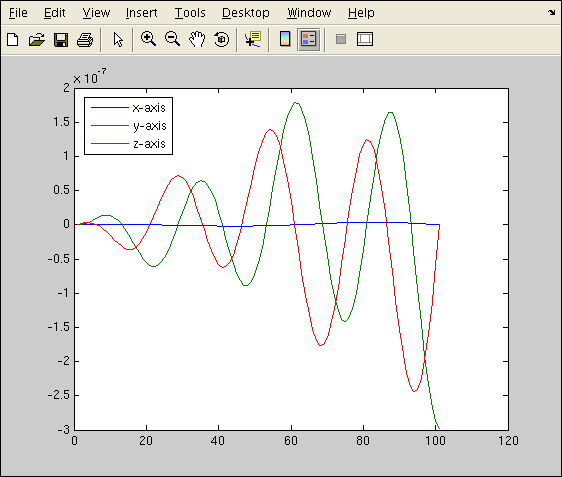
\includegraphics[width=80mm]{figures/relative6_vba.png}
        \caption{The variation with time of the difference between the analytical and numerical solutions for the velocity of B with respect to A.}
        \label{fig:rel6_4} 
  \end{center}
\end{figure}

 \begin{figure}[!ht]
  \begin{center}
        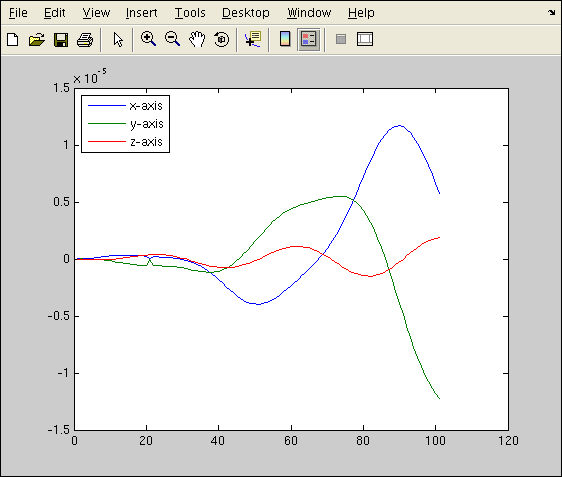
\includegraphics[width=80mm]{figures/relative7_xab.png}
        \caption{The variation with time of the difference between the analytical and numerical solutions for the position of A with respect to B.}
        \label{fig:rel7_1}
  \end{center}
\end{figure}

 \begin{figure}[!ht]
  \begin{center}
        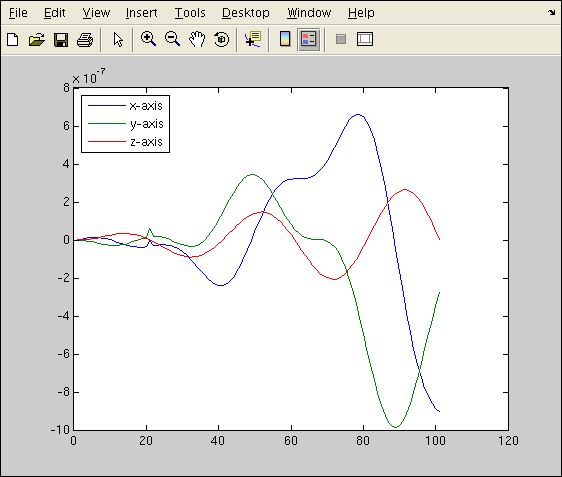
\includegraphics[width=80mm]{figures/relative7_vab.png}
        \caption{The variation with time of the difference between the analytical and numerical solutions for the velocity of A with respect to B.} 
  \end{center}
\end{figure}

 \begin{figure}[!ht]
  \begin{center}
        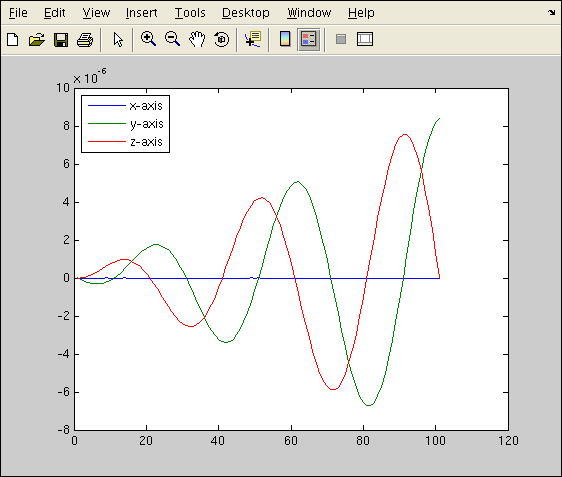
\includegraphics[width=80mm]{figures/relative7_wab.png}
        \caption{The variation with time of the difference between the analytical and numerical solutions for the angular velocity of A with respect to B.} 
  \end{center}
\end{figure}

\begin{figure}[!ht]
  \begin{center}
        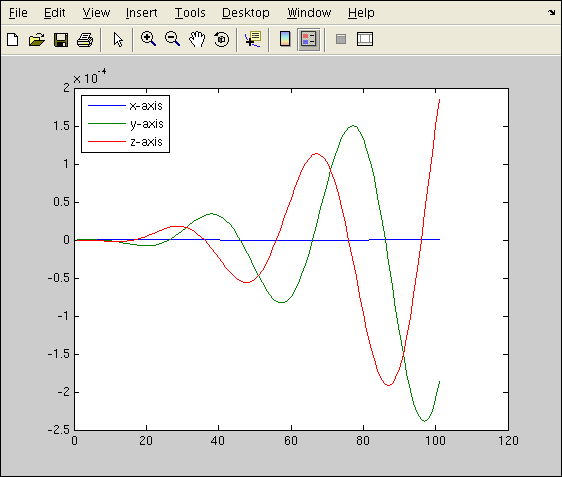
\includegraphics[width=80mm]{figures/relative7_xba.png}
        \caption{The variation with time of the difference between the analytical and numerical solutions for the position of B with respect to A.} 
  \end{center}
\end{figure}

 \begin{figure}[!ht]
  \begin{center}
        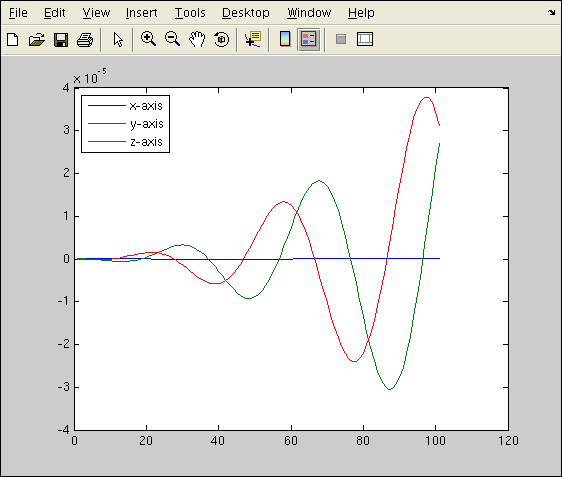
\includegraphics[width=80mm]{figures/relative7_vba.png}
        \caption{The variation with time of the difference between the analytical and numerical solutions for the velocity of B with respect to A.} 
  \end{center}
\end{figure}

\begin{figure}[!ht]
  \begin{center}
        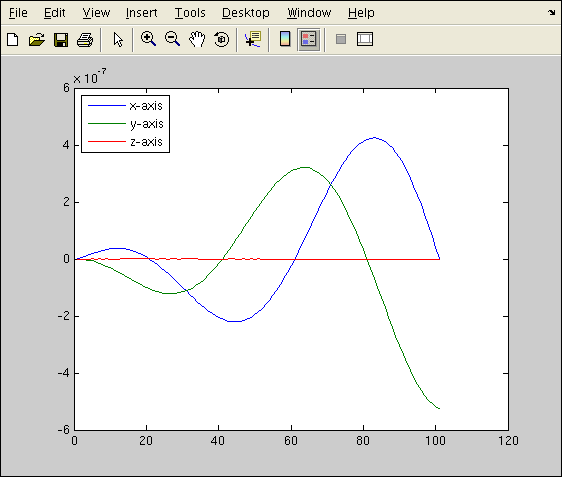
\includegraphics[width=80mm]{figures/relative7_wba.png}
        \caption{The variation with time of the difference between the analytical and numerical solutions for the angular velocity of B with respect to A.}
        \label{fig:rel7_6} 
  \end{center}
\end{figure}

\end{description}


%\section{Validation}
%%%%%%%%%%%%%%%%%%%%%%%%%%%%%%%%%%%%%%%%%%%%%%%%%%%%%%%%%%%%%%%%%%%%%%%%%%%%%%%%%
%
% Purpose:  Validation part of V&V for the Relative model
%
% 
%
%%%%%%%%%%%%%%%%%%%%%%%%%%%%%%%%%%%%%%%%%%%%%%%%%%%%%%%%%%%%%%%%%%%%%%%%%%%%%%%%

\section{Validation}

There is no independent validation of the \RelativeDesc.




\part{\SolarBetaDescT}



%----------------------------------
\chapter{Introduction}\label{ch:SolarBetaintro}
%----------------------------------

\section{Purpose and Objectives of the \SolarBetaDescT}
%%%%%%%%%%%%%%%%%%%%%%%%%%%%%%%%%%%%%%%%%%%%%%%%%%%%%%%%%%%%%%%%%%%%%%%%%%%%%%%%%
%
% Purpose:  Introduction for the SolarBeta model.
%
% 
%
%%%%%%%%%%%%%%%%%%%%%%%%%%%%%%%%%%%%%%%%%%%%%%%%%%%%%%%%%%%%%%%%%%%%%%%%%%%%%%%%


%\section{Purpose and Objectives of \SolarBetaDesc}
% Incorporate the intro paragraph that used to begin this Chapter here. 
% This is location of the true introduction where you explain what this model 
% does.

Spacecraft with movable solar panels and thermal radiators
continuously rotate the solar panels to catch as much sunlight as possible
and rotate the thermal radiators to catch as little sunlight as possible.
The varying orientations of these devices present ever changing cross sections
to atmospheric drag. Properly modeling the orientation of these devices
improves the fidelity of simulation of such spacecraft.

One of the principal drivers of these panel orientations is the angle between
the vector toward the sun and the spacecraft's orbital plane, which is called
the {\em solar beta angle}. The \SolarBetaDesc\ represents this angle.

This part of the document describes the \SolarBetaDesc\ developed for use with \JEODid.

















%----------------------------------
\chapter{Product Requirements}\label{ch:SolarBetareqt}
%----------------------------------


%%%%%%%%%%%%%%%%%%%%%%%%%%%%%%%%%%%%%%%%%%%%%%%%%%%%%%%%%%%%%%%%%%%%%%%%%%%%%%%%%
%
% Purpose:  requirements for the SolarBeta model
%
% 
%
%%%%%%%%%%%%%%%%%%%%%%%%%%%%%%%%%%%%%%%%%%%%%%%%%%%%%%%%%%%%%%%%%%%%%%%%%%%%%%%%

% add text here to describe general model requirements
% text is of the form:
\requirement{Solar Beta representation}
\label{reqt:SolarBeta}
\begin{description}
  \item[Requirement:]\ \newline
     The Solar Beta Derived State will provide the capability for calculating the Solar Beta angle associated with the vehicle's current state.
  \item[Rationale:]\ \newline
     Capability from JEOD 1.5.
  \item[Verification:]\ \newline
     Test
\end{description}

\section{Requirements Traceability}

\begin{longtable}[c]{||p{3.5in}|p{3.5in}|}
\caption{Requirements Traceability} \\[6pt]
\hline
{\bf Requirement} & {\bf Inspection and Testing} \\ 
\hline \hline
\endhead
\ref{reqt:SolarBeta} - Solar Beta representation &
  Test~\ref{test:solarbetalongterm} \\ 
  & Test~\ref{test:solarbetacompare} \\ \hline

\end{longtable}




%----------------------------------
\chapter{Product Specification}\label{ch:SolarBetaspec}
%----------------------------------

\section{Conceptual Design}
%%%%%%%%%%%%%%%%%%%%%%%%%%%%%%%%%%%%%%%%%%%%%%%%%%%%%%%%%%%%%%%%%%%%%%%%%%%%%%%%%
%
% Purpose:  Conceptual part of Product Spec for the SolarBeta model
%
% 
%
%%%%%%%%%%%%%%%%%%%%%%%%%%%%%%%%%%%%%%%%%%%%%%%%%%%%%%%%%%%%%%%%%%%%%%%%%%%%%%%%


%\section{Conceptual Design}

The Solar Beta angle, $\beta$, is the angle between the Sun-vector (the vector from the center of Earth to Sun), and the projection of the Sun-vector onto the orbital plane.  An alternative view is to consider $\beta$ as $\pi /2 - \alpha$, where $\alpha$ is the angle between the orbital angular momentum vector and the Sun vector.  See Figure~\ref{fig:solarbetaintro} for a graphical representation.

\begin{figure}[htp]
\begin{center}
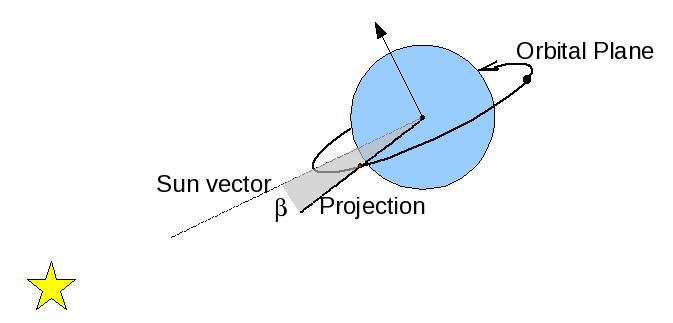
\includegraphics[width=5in]{figures/solar_beta.jpg}
\caption{The definition of the Solar Beta angle.  The arrow represents the orbital angular momentum vector.  Note that the position of the vehicle (upper right) on the orbit is of no consequence to the determination of the Solar Beta angle.}
\label{fig:solarbetaintro}
\end{center}
\end{figure}

$\beta$ is positive when the Sun-vector is above the orbital plane (i.e., when it is aligned in the same general sense as the orbital angular momentum vector, also interpreted as when the dot product of these two vectors is positive), zero when the Sun-vector lies in the orbital plane, and negative when the Sun-vector lies below the orbital plane.  $\beta \in \left[ -\frac{\pi}{2}, \frac{\pi}{2} \right]$.  

$\beta$ is affected by orbital precession, and by the orbital motion of Earth with respect to Sun.  It is not directly affected by the vehicle's position on its orbit.

As an illustration, consider a vehicle in an equatorial orbit.  At the equinoxes, the Sun-vector lies in the orbital plane, and $\beta = 0$.  In the Northern summer (April - September), the sun lies above the equator, hence above the orbit (assuming that the orbit is in the same sense as Earth's rotation), and $\beta > 0$, reaching a peak at the solstice.  In the Southern summer (October - March), the sun is below the equator, hence below the orbit, and $\beta < 0$, reaching a minimum at the solstice.

The effect of precession and time of year can be seen in Figure~\ref{fig:solarbetaISS}, which shows the typical variation with time of the Solar beta angle for a vehicle in an orbit comparable to that of the International Space Station.

\begin{figure}[htp]
\begin{center}
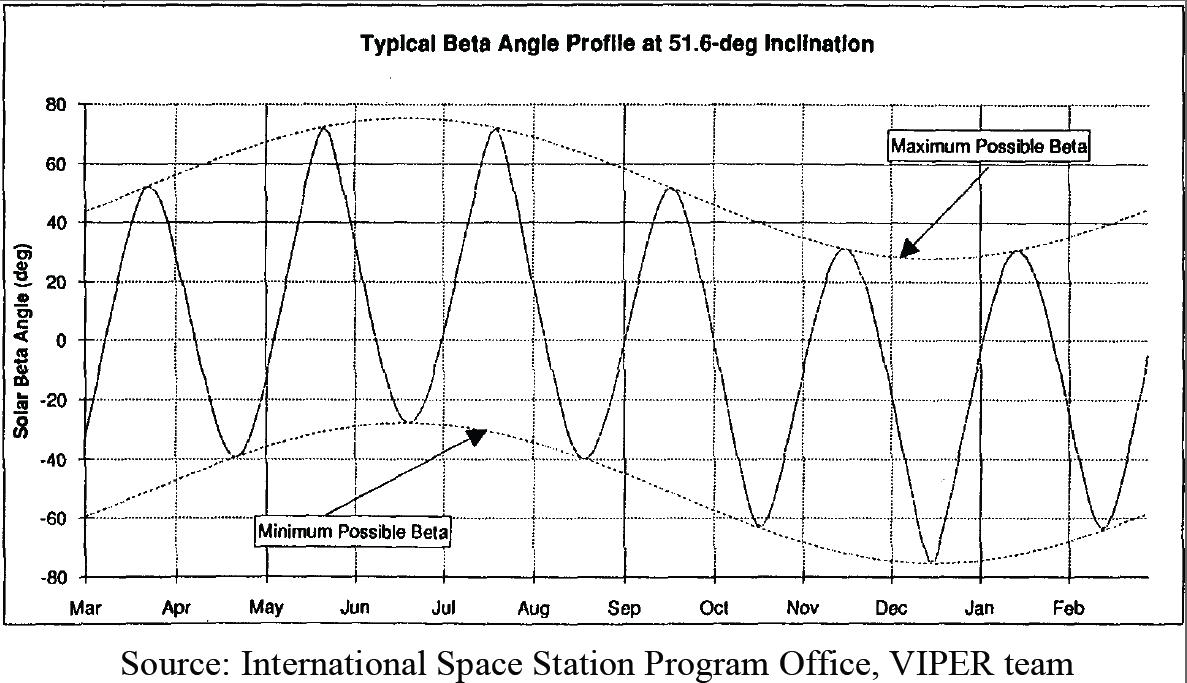
\includegraphics[width=5in]{figures/solar_beta_iss.jpg}
\caption{The variation with time of the Solar Beta angle for an orbit with inclination of 51.6 degrees.  The high frequency oscillation is due to precession, and the long period variation due to Earth's motion around Sun.}
\label{fig:solarbetaISS}
\end{center}
\end{figure}


%\section{Mathematical Formulations}
%%%%%%%%%%%%%%%%%%%%%%%%%%%%%%%%%%%%%%%%%%%%%%%%%%%%%%%%%%%%%%%%%%%%%%%%%%%%%%%%%
%
% Purpose:  Mathematical Formulation part of Product Spec for the SolarBeta model
%
% 
%
%%%%%%%%%%%%%%%%%%%%%%%%%%%%%%%%%%%%%%%%%%%%%%%%%%%%%%%%%%%%%%%%%%%%%%%%%%%%%%%%

\section{Mathematical Formulations}\label{sec:solarbetamath}

The mathematical algorithm for computing the Solar Beta angle is straightforward, and builds on tools developed in other models.

While Solar Beta is typically defined (and used) for Earth-orbiting situations, the same concepts can easily be extended to any other planet.  Therefore, the code is written in such a way as to make the ``host'' planet a user-defined quantity.  Throughout this description, we will refer to \textit{planet}; for most applications, this can be read as \textit{Earth}.  

First, the position of \textit{sun} with respect to \textit{planet} is determined using the \textit{compute\_position\_from} method from the \textit{Planet} model (see the \href{file:\JEODHOME/models/environment/planet/docs/planet.pdf}{\em Planet model documentation}~\cite{dynenv:PLANET} for details), and the state of the vehicle with respect to \textit{planet} is determined using the \textit{compute\_relative\_state} method from the \textit{DynBody} model (see the \href{file:\JEODHOME/models/dynamics/dyn_body/docs/dyn_body.pdf}{\em Dynamics Body documentation}~\cite{dynenv:DYNBODY} for details).  Both relative positions are represented in the inertial reference frame (origin is not relevant since these are relative positions).

Denote $\vec {r}_{A,B}$ as the position of object A with respect to B.

The specific angular momentum of the vehicle due to its orbital motion about the specified planetary body is calculated from a straightforward vector (cross) product of position with velocity.  Since the state is recorded in the inertial reference frame centered on the planet, the angular momentum will also be expressed in the inertial reference frame (origin is not relevant).  Note, however, that while the definition of Solar Beta breaks down when the vehicle is not in orbit about its specified planet, this calculation continues to be completely valid.  Verifying that the vehicle is in orbit would be computationally expensive, and this verification IS NOT carried out.  It is left to the user to ensure that the vehicle is, in fact, in orbit about the specified planet

\begin{equation*}
\vec{h} = \vec{r}_{veh,planet} \times \vec{v}_{veh,planet}
\end{equation*}

Next, the scalar product of the specific angular momentum and sun-planet vectors is taken, and manipulated to provide $\beta$.

\begin{equation*}
\vec{h} \cdot \vec{r}_{sun,planet} = \left|\vec{h}\right|\left|\vec{r}_{sun,planet}\right|cos\alpha = \left|\vec{h}\right|\left|\vec{r}_{sun,planet}\right| sin\beta
\end{equation*}
\begin{equation}
\beta = sin^{-1} \left( \frac{\vec{h} \cdot \vec{r}_{sun,planet}}{\left|\vec{h}\right|\left|\vec{r}_{sun,planet}\right|} \right)
\end{equation}

%\section{Detailed Design}

%%%%%%%%%%%%%%%%%%%%%%%%%%%%%%%%%%%%%%%%%%%%%%%%%%%%%%%%%%%%%%%%%%%%%%%%%%%%%%%%%
%
% Purpose:  Detailed part of Product Spec for the SolarBeta model
%
% 
%
%%%%%%%%%%%%%%%%%%%%%%%%%%%%%%%%%%%%%%%%%%%%%%%%%%%%%%%%%%%%%%%%%%%%%%%%%%%%%%%%

\section{Detailed Design}
See the \href{file:refman.pdf}{Reference Manual}\cite{derivedstatebib:ReferenceManual} for a summary of member data and member methods for all classes.  

\subsection{Process Architecture}
The process architecture for the \SolarBetaDesc\ is trivial, comprising operationally independent methods.

\subsection{Functional Design}
This section describes the functional operation of the methods in each class.

The \SolarBetaDesc\ contains only one class:
\begin{itemize}
\classitem{SolarBetaDerivedState}
\textref{DerivedState}{ref:DerivedState}

This contains only the methods \textit{initialize} and \textit{update}:
\begin{enumerate}
\funcitem{initialize}
The initialization process comprises the following steps:
\begin{enumerate}
\item{} The generic DerivedState initialization routine is called to establish the naming convention of the reference object (i.e., the planet about which the vehicle is orbiting) and state identifier.
\item{} The registry of active bodies, maintained by the Dynamics Manager (see \href{file:\JEODHOME/models/dynamics/dyn_manager/docs/dyn_manager.pdf}{\em Dynamics Manager Documentation}~\cite{dynenv:DYNMANAGER}) is updated to ensure that the ephemeris of the sun and the reference body are both being updated.
\end{enumerate}

\funcitem{update}
The process at update is described entirely in the \reftext{Mathematical Formulations}{sec:solarbetamath} section.


\end{enumerate}
\end{itemize}






\chapter{User's Guide}\label{ch:SolarBetauser}
%----------------------------------
The Analysis section of the User's Guide is intended primarily for
users of pre-existing simulations.  
It contains: 
\begin{itemize}
\item A description of how to modify \SolarBetaDesc\ variables after
the simulation
has compiled, including an in-depth discussion of the input file,
\item An overview of how to interpret (but not edit) the S\_define
file,
\item A sample of some of the typical variables that may be logged.
\end{itemize}

The Integration section of the User's Guide is intended for simulation
developers.
It describes the necessary configuration of the \SolarBetaDesc\
within an
S\_define file, and the creation of standard run directories.  The
latter
component assumes a thorough understanding of the preceding Analysis
section of the user guide.
Where applicable, the user may be directed to selected portions of
Product Specification (Chapter \ref{ch:SolarBetaspec}).

The Extension section of the User's Guide is intended primarily for
developers
needing to extend the capability of the \SolarBetaDesc.  Such users
should have a
thorough understanding of how the model is used in the preceding
Integration section, and of the model
specification (described in Chapter \ref{ch:SolarBetaspec}).


\section{Analysis}
%%%%%%%%%%%%%%%%%%%%%%%%%%%%%%%%%%%%%%%%%%%%%%%%%%%%%%%%%%%%%%%%%%%%%%%%%%%%%%%%%
%
% Purpose:  Analysis part of User's Guide for the SolarBeta model
%
% 
%
%%%%%%%%%%%%%%%%%%%%%%%%%%%%%%%%%%%%%%%%%%%%%%%%%%%%%%%%%%%%%%%%%%%%%%%%%%%%%%%%

% \section{Analysis}
\label{sec:solarbetauseranalysis}

\subsection{Identifying the \SolarBetaDescT}
If Solar Beta has been included in the simulation, there will be an instance of \textit{SolarBetaDerivedState} located in the S\_define file.  This would typically be found in either the vehicle object, or a separate relative-state object.  There should be an accompanying call to an initialization routine, which takes a reference to the vehicle as one if its inputs.  The reference body is defined elsewhere, possibly in the input file.

Example:
\begin{verbatim}
sim_object{
dynamics/derived_state:    SolarBetaDerivedState example_of_solar_beta;

(initialization) dynamics/derived_state:
example_of_rel_state_object.example_of_solar_beta.initialize (
    Inout DynBody &      subject_body = vehicle_object.dyn_body,
    Inout DynManager &   dyn_manager  = manager_object.dyn_manager);
    
{environment}
example_of_rel_state_object.example_of_solar_beta.update ( )

} example_of_rel_state_object;
\end{verbatim}

Then the input file may have a line comparable to:
\begin{verbatim}
example_of_rel_state_object.example_of_solar_beta.reference_name = "Earth";
\end{verbatim}


\subsection{Editing the \SolarBetaDescT}
There is very little to edit in the \SolarBetaDesc.  The \textit{reference\_name} should match the planet around which the vehicle is orbiting; if it does not, that may be changed.

There is also an \textit{active} flag that can be set to turn on or off the calculation of the Solar Beta angle.  If the \SolarBetaDesc\ appears in the simulation, but is not outputting time-varying data (and remember, this data will vary very slowly because it depends on the precession of the orbit, and on the position of the reference planet with respect to Sun), then it may be that the model is inactive. 

\subsection{Output Data}
The only data intended for usable output is the variable \textit{solar\_beta}, the Solar Beta angle.


%\section{Integration}
%%%%%%%%%%%%%%%%%%%%%%%%%%%%%%%%%%%%%%%%%%%%%%%%%%%%%%%%%%%%%%%%%%%%%%%%%%%%%%%%%
%
% Purpose:  Integration part of User's Guide for the SolarBeta model
%
% 
%
%%%%%%%%%%%%%%%%%%%%%%%%%%%%%%%%%%%%%%%%%%%%%%%%%%%%%%%%%%%%%%%%%%%%%%%%%%%%%%%%

 \section{Integration}
Including the \SolarBetaDesc\  into the simulation is very straightforward.

 \subsection{Generating the S\_define}

Conventional practice would add the \SolarBetaDesc\ to a specific vehicle, or, if there are multiple relative states between different vehicles such that a relative-state object becomes desirable, it could be added into that relative-state object.

The instance of \textit{SolarBetaDerivedState} needs to be defined, the model initialized, and a routine update scheduled.  An example of how this may look is found in the \textit{Analysis} section (\ref{sec:solarbetauseranalysis}).  Examples of how to include the Solar Beta within the vehicle object are found in the Solar Beta Verification simulations, released with \JEODid.

\subsection{Generating the Input File}
The only value necessary to define in the input file (or in Modified Data) is the name of the reference object.  The reference object MUST BE the planet about which the vehicle is orbiting. The calculations determine the orbit based on the angular momentum of the vehicle about the reference object.  If the vehicle is orbiting a different object, the angular momentum will still be calculated based on the reference object, which will produce results not at all relevant to the problem.

The example given in the \textref{Analysis}{sec:solarbetauseranalysis} section is
\begin{verbatim}
example_of_rel_state_object.example_of_solar_beta.reference_name = "Earth";
\end{verbatim}

\subsection{Logging the Data}
There is only one variable for output, that is the Solar Beta angle itself.  Continuing with the example in the \textref{Analysis}{sec:solarbetauseranalysis} section, log
\begin{verbatim}
example_of_rel_state_object.example_of_solar_beta.solar_beta.
\end{verbatim}


%\section{Extension}
%%%%%%%%%%%%%%%%%%%%%%%%%%%%%%%%%%%%%%%%%%%%%%%%%%%%%%%%%%%%%%%%%%%%%%%%%%%%%%%%%
%
% Purpose:  Extension part of User's Guide for the SolarBeta model
%
% 
%
%%%%%%%%%%%%%%%%%%%%%%%%%%%%%%%%%%%%%%%%%%%%%%%%%%%%%%%%%%%%%%%%%%%%%%%%%%%%%%%%

 \section{Extension}

It is not anticipated that the \SolarBetaDesc\ be extended; the angle is independent of the vehicle or the position of the vehicle on its orbit.  Extension beyond Earth orbit is already included; it is as easy to compute Solar Beta angles with respect to any other planetary body (for example, for Lunar orbiting vehicles) as it is for Earth.  

The other feasible extension would be to replace Sun with some other planetary body.  This could be desirable for obtaining orientation data when pointing toward other planetary objects is important, but it would no longer be a ``Solar'' Beta angle.  To implement this extension, copy the \SolarBetaDesc\ to generate a new model, rename the variable \textit{sun} to something more suitable, and change the value \textit{``Sun''} in the \textit{initialize} method to the name of the target object.

%----------------------------------
\chapter{Verification and
Validation}\label{ch:SolarBetaivv}
%----------------------------------

\section{Verification}
%%%%%%%%%%%%%%%%%%%%%%%%%%%%%%%%%%%%%%%%%%%%%%%%%%%%%%%%%%%%%%%%%%%%%%%%%%%%%%%%%
%
% Purpose:  Verification part of V&V for the SolarBeta model
%
% 
%
%%%%%%%%%%%%%%%%%%%%%%%%%%%%%%%%%%%%%%%%%%%%%%%%%%%%%%%%%%%%%%%%%%%%%%%%%%%%%%%%

% \section{Verification}

%%% code imported from old template structure
%\inspection{<Name of Inspection>}\label{inspect:<label>}
% <description> to satisfy  
% requirement \ref{reqt:<label>}.

Given the simplicity of the model, a single simulation can be used for all of the verification and validation tests.  The initialization of some aspects, such as solar and lunary gravity, is redundant for some tests, but having one simulation simplifies that validation greatly.  The simulation uses the DE405 ephemeris model to compute planetary ephemeris and simulates an orbital body as a ``falling rock'' orbiting the Earth for up to a year.

\test{Long-Term Behavior}
\label{test:solarbetalongterm}
\begin{description}
\item{Purpose:} \\
The purpose of this test is to verify the solar beta angle characteristics
and accuracy over a period of time. 

\item{Requirements} \\
The succesful outcome of this test, together with the validation Test~\ref{test:solarbetacompare} satisfy requirement~\ref{reqt:SolarBeta}.
\item{Procedure:} \\
The simulation is run for one
year with different orbital inclinations and gravity modeled as
spherical or 8x8, with solar and lunar gravitational perturbations on and off.

\item{Predictions:}
\begin{enumerate}
 \item {Equatorial orbit, spherical gravity} \ \newline
The Solar Beta will show a single cycle of variation associated with the orbit (which has a fixed-orientation in an inertial frame) passing once around the sun.  The magnitude of that oscillation should be equal to the tilt of Earth's axis with respect to the ecliptic, $23.44^\circ$
\item{Inclined orbit, $23.4^\circ$, non-spherical gravity} \ \newline
The Solar Beta will oscillate more rapidly as the orbital plane precesses in the non-spherical gravitational field.  This should cause an additional oscillation of $23.4^\circ$ due to the orbital inclination \textit{on top of} the annual variation due to the orientation of the equator as expected from the previous case.  
\item{Inclined orbit, $51.6^\circ$, non-spherical gravity} \ \newline
This case should be comparable to the previous case, with a longer-term precession, and larger oscillation about the equatorial oscillation seen in the first case. 
\item{Inclined orbit, $23.4^\circ$, spherical gravity, lunar and solar gravitational perturbation on} \ \newline
Several cases were run for comparison
\begin{enumerate}
 \item Inclined orbit, $23.4^\circ$,  with spherical gravity.
 \item Inclined orbit, $23.4^\circ$,  with spherical gravity, and the addition of lunar gravitational perturbations.
 \item Inclined orbit, $23.4^\circ$,  with spherical gravity, and the addition of lunar and solar gravitational perturbations.
\end{enumerate}
All of these should show an annual variation, with small oscillations induced by the gravitational perturbations to the orbit. 

\end{enumerate}

\item{Results:}
\begin{enumerate}
 \item {Equatorial orbit, spherical gravity} \ \newline
Data is as expected, see Figure~\ref{fig:solbeta123} for comparison of cases 1, 2, and 3.
\item {Inclined orbit, $23.4^\circ$, non-spherical gravity} \ \newline
Data is as expected, see Figure~\ref{fig:solbeta123} for comparison of cases 1, 2, and 3.  The figure shows an appropriately scaled short-period oscillation superposed on the long-period (annual) oscillation.
\item {Inclined orbit, $51.6^\circ$, non-spherical gravity} \ \newline
Data is as expected, see Figure~\ref{fig:solbeta123} for comparison of cases 1, 2, and 3.  The figure shows an appropriately scaled short-period oscillation superposed on the long-period (annual) oscillation.  The short-period oscillation has larger period than for the less inclined orbit.  Similar runs for orbits inclined at 70, 85, and 90 degrees continued the trend, with more pronounced variation in the Solar beta angle, and longer duration precession, gradually slowing until no orbital precession was evident at 90 degrees.
\item{Gravitational Perturbations} \ \newline
The effect of graviational perturbations on the orientation of the orbit are small; the addition of lunar perturbations has more effect than the addition of solar perturbations.
\end{enumerate}
\end{description}

\begin{figure}[!ht]
  \begin{center}
        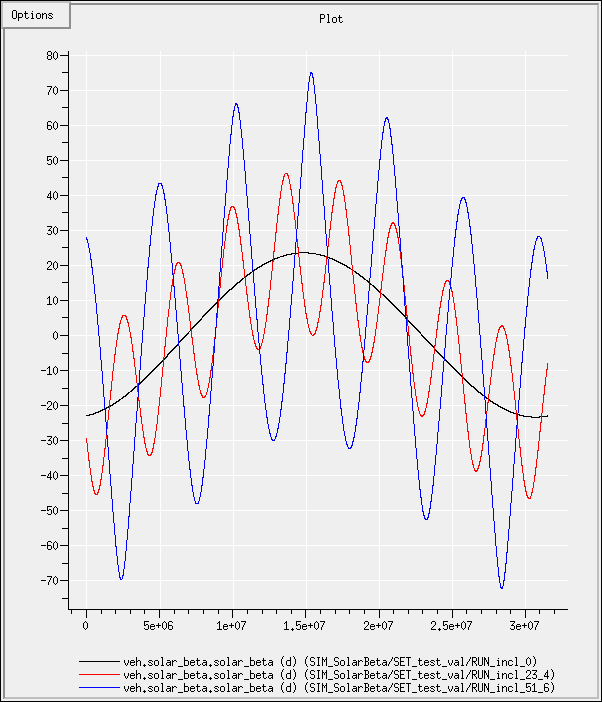
\includegraphics[width=80mm]{figures/solbeta123.jpg}
        \caption{The variation of Solar Beta with time for the first three test cases.  These are all circular orbits with orbital inclinations of 0, 23.4, and 51.6 degrees respectively} 
        \label{fig:solbeta123}
  \end{center}
\end{figure}


%\section{Validation}
%%%%%%%%%%%%%%%%%%%%%%%%%%%%%%%%%%%%%%%%%%%%%%%%%%%%%%%%%%%%%%%%%%%%%%%%%%%%%%%%%
%
% Purpose:  Validation part of V&V for the SolarBeta model
%
%
%
%%%%%%%%%%%%%%%%%%%%%%%%%%%%%%%%%%%%%%%%%%%%%%%%%%%%%%%%%%%%%%%%%%%%%%%%%%%%%%%%

\section{Validation}

\test{Comparison with External Data}
\label{test:solarbetacompare}
\begin{description}
\item{Purpose:} \\
The purpose of this test is to compare solar beta angles
calculated by this model with externally-provided values.

\item{Requirements:} \ \newline
The succesful outcome of this test, together with the validation Test~\ref{test:solarbetalongterm} satisfy requirement~\ref{reqt:SolarBeta}.

\item{Procedure:}\ \newline
Several tests are carried out, including:
\begin{enumerate}
\item{RUN\_comp\_ISS} \ \newline
This run compares against the Solar Beta for ISS, using a simple ephemeris model.
The reference data from The Flight Operation Directorate at NASA JSC 
provides a solar beta value for a given ISS state (inertial position/velocity)
at a given date. The underlying program uses a simple ephemeris model,
resulting in solar beta angles accurate to within 1 degree.
The vehicle state and time as portrayed in
Figure~\ref{fig:STS_114_ISS} were used to initialize the test simulation
and to validate the results.

\begin{figure}
\centering
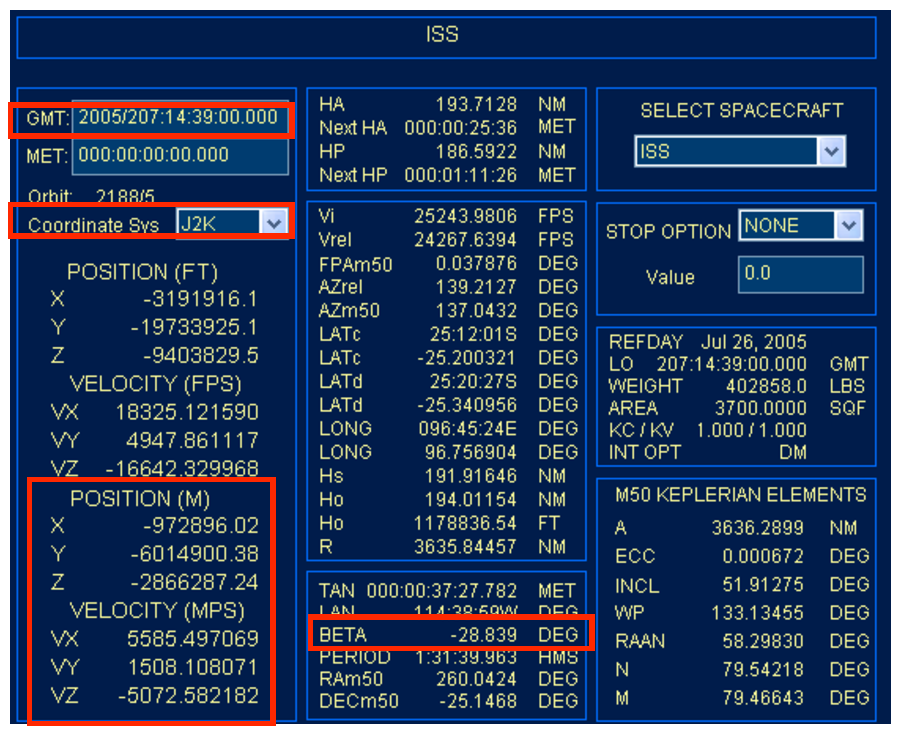
\includegraphics{figures/SOLAR_BETA_fig5}
\caption{Mission Operations ISS State and Solar Beta}
\label{fig:STS_114_ISS}
\end{figure}

\item{RUN\_comp\_STS121a and RUN\_comp\_STS121b] STS-121} \ \newline
These runs compare against the Solar Beta for ISS, generated using the DE405 ephemeris
The Mission Operations Directorate uses the DE405 ephemeris
to compute solar beta angles in flight-certified applications.
Mission STS-121 data, provided by William H. Tracy/NASA/JSC/DM32,
provided solar beta values for a pair of given STS-121 states.

The vehicle state and time as portrayed in
figures~\ref{fig:STS_121a} and~\ref{fig:STS_121b} were used to initialize
the test simulation and to validate the results.
\end{enumerate}

\item{Predictions:}
\begin{enumerate}
\item{RUN\_comp\_ISS} \ \newline
The Solar Beta angles generated by the
simple ephemeris model are accurate to within one degree compared to
angles computed with the aid of the highly accurate DE405 ephemeris model.

Therefore, the solar beta angle computed using the \SolarBetaDesc\ should differ with
the externally-provided value by no more than one degree
for this test case.

\item{RUN\_comp\_STS121a and RUN\_comp\_STS121b}\ \newline
Solar beta angles generated externally using the DE405 ephemeris model
should agree with angles computed by the \SolarBetaDesc\ to a very high degree.
The validation data for these tests provide initial conditions in the M50 reference frame, whereas \JEODid\ uses the J2000 frame.  A conversion of the specification state from M50 to J2000 serves as the initialization data for these tests.  This incorporates a potential source of error.
Other sources of error are in the state vector and the epoch time.
The externally-provided data give solar beta angles with three
decimal places of precision (that is, $1/1000^{th}$ degree).  The initial state and Solar Beta angle for these two tests are shown in Figures~\ref{fig:STS_121a} and~\ref{fig:STS_121b}.

Even accounting for the potential errors introduced by the precision in the specification of the epoch time, and of the M50 state, and further, its conversion to J2000 conversion, the solar beta angle computed using the \SolarBetaDesc\ should differ with the externally-provided value by no more than $0.001^\circ$ for these test cases.
\end{enumerate}

\item{Results:}
\begin{enumerate}
\item{RUN\_comp\_ISS}\\
 The solar beta angle calculated by the simulation at
initialization time was $-28.41^\circ$, which, to within $1^\circ$,
agrees with the externally- supplied value of $-28.839^\circ$.

\item{RUN\_comp\_STS121a and RUN\_comp\_STS121b} \\
The solar beta angles calculated by the simulation at initialization time are
$5.29269^\circ$ (RUN\_comp\_STS121a) and $3.85718^\circ$ (RUN\_comp\_STS121b),
which, to $0.001^\circ$, compare exactly the externally-supplied values
of $5.293^\circ$ and $3.857^\circ$
\end{enumerate}
All test cases pass their respective test criterion.
\end{description}


\begin{figure}
\centering
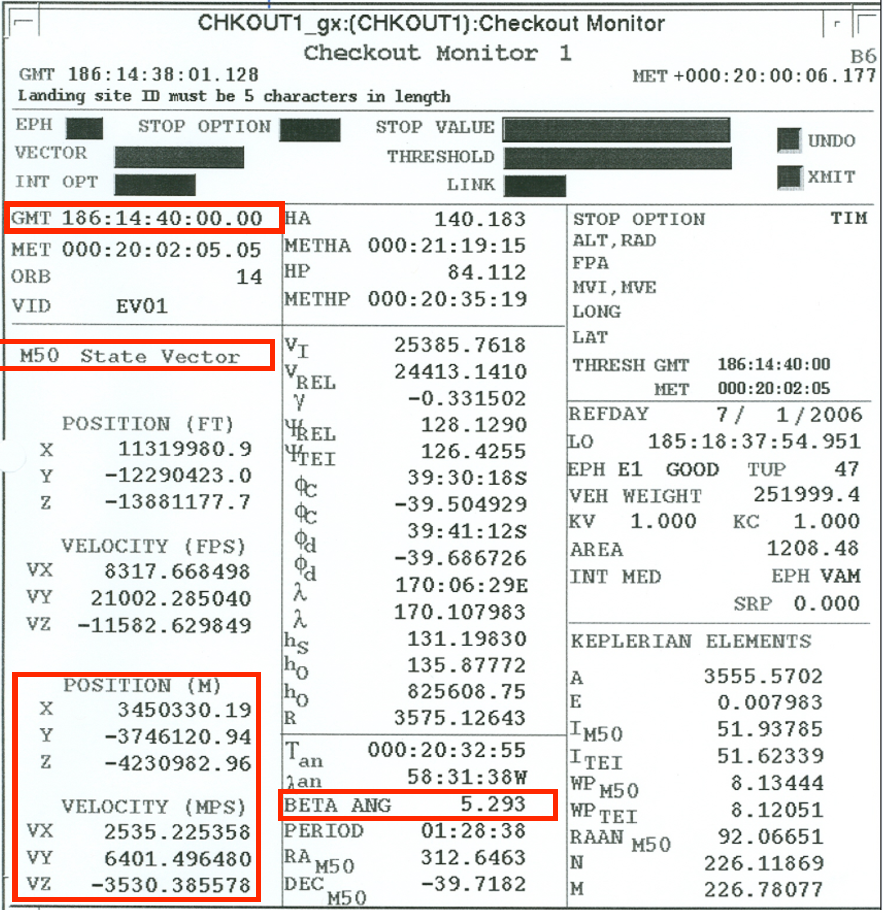
\includegraphics{figures/SOLAR_BETA_fig6}
\caption{Mission Operations STS-121 Checkout Monitor Data}
\label{fig:STS_121a}
\end{figure}


\begin{figure}
\centering
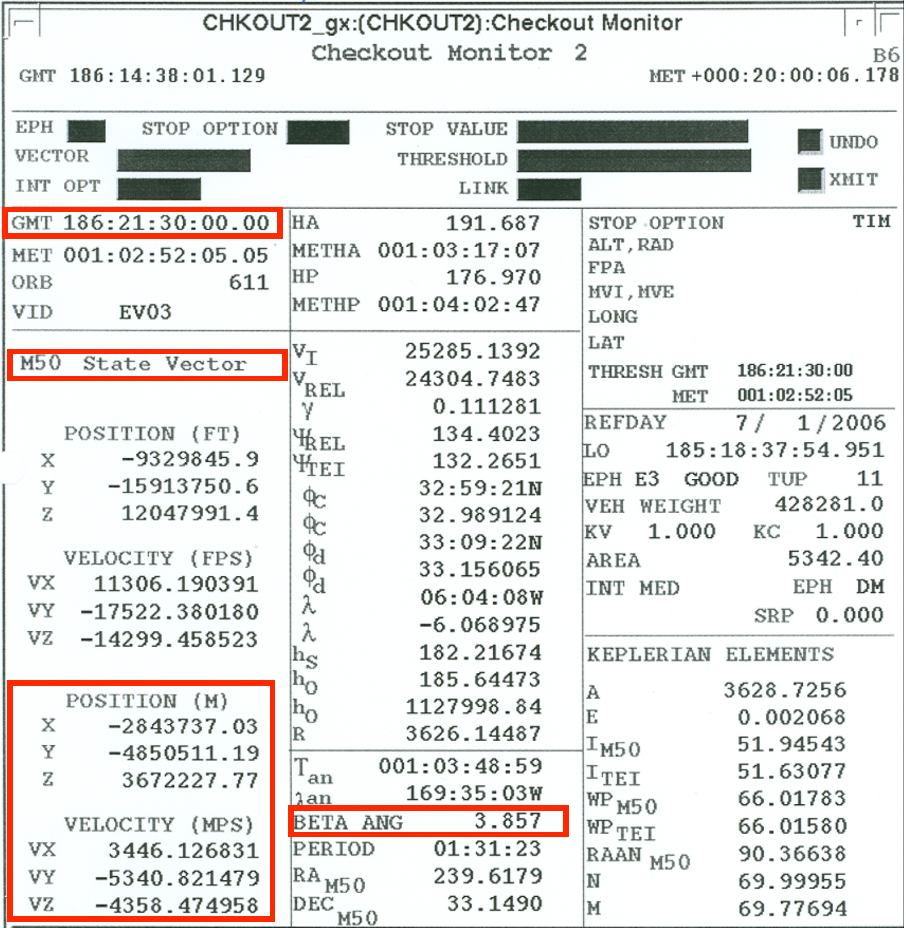
\includegraphics{figures/SOLAR_BETA_fig7}
\caption{Mission Operations STS-121 Checkout Monitor Data}
\label{fig:STS_121b}
\end{figure}

\clearpage





%%%%%%%%%%%%%%%%%%%%%%%%%%%%%%%%%%%%%%%%%%%%%%%%%%%%%%%%%%%%%%%%%%%%%%%%%
% Bibliography
%%%%%%%%%%%%%%%%%%%%%%%%%%%%%%%%%%%%%%%%%%%%%%%%%%%%%%%%%%%%%%%%%%%%%%%%%
\newpage
\pdfbookmark{Bibliography}{bibliography}
\bibliography{dynenv,DerivedState}
\bibliographystyle{plain}

%\pagebreak
%\appendix

\end{document}
